\clearpage
\appendix
\section{Distribution Gallery for This Session}
This appendix collects the distribution-style outputs generated in this session. Exact statevector plots show true top-$k$ bitstring probabilities. Aer MPS plots show empirical sample counts, so their probabilities are count estimates. The MPS-distillation plots aggregate counts across seeds, shot counts, and bond dimensions. The peaked-circuit plots are different: they are one-qubit marginal distributions, not full bitstring distributions; their candidate is formed by thresholding each qubit at $P(1)=0.5$.

\subsection{How to Read These Plots}
\begin{itemize}
  \item A tall rank-1 bar separated from rank 2 is strong evidence for the exact or sampled peak.
  \item Repeated MPS winners across seeds/settings are more useful than a single top sample.
  \item If every sampled bitstring is unique, the plotted top bitstring is not reliable peak evidence.
  \item In peaked-circuit marginal plots, any bar close to $0.5$ is a bit-level warning. This is exactly why \code{24\_13} was one bit off.
  \item Cancelled or partial jobs produced JSON/logs but no trustworthy distribution figure; those are documented in \code{outputs/peaked\_circuit\_sim\_all/RUN\_LOG.md}.
\end{itemize}

\subsection{Exact Statevector Top-k Distributions}
\begin{figure}[H]
\centering
\begin{minipage}{0.48\linewidth}
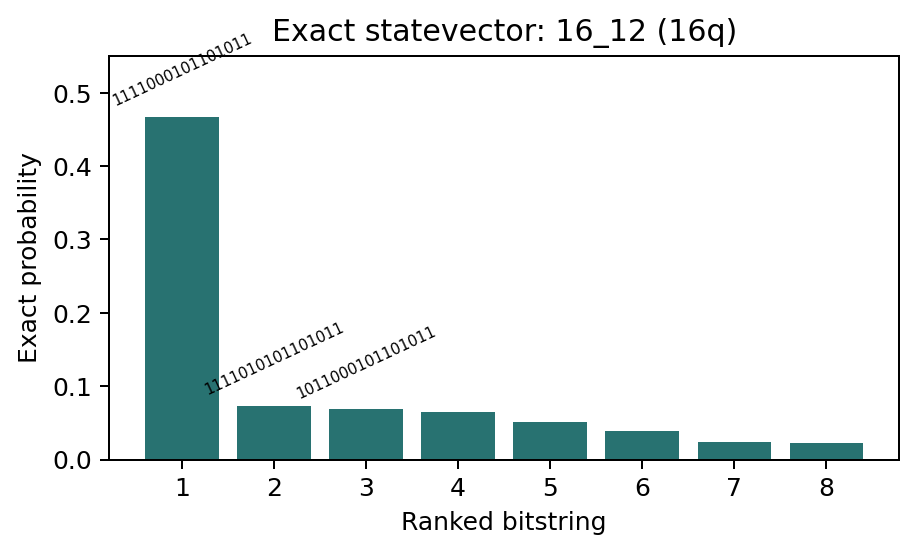
\includegraphics[width=\linewidth]{figures/appendix_exact/exact_16_12.png}
\caption*{\code{16\_12}: exact statevector top probabilities.}
\end{minipage}\hfill
\begin{minipage}{0.48\linewidth}
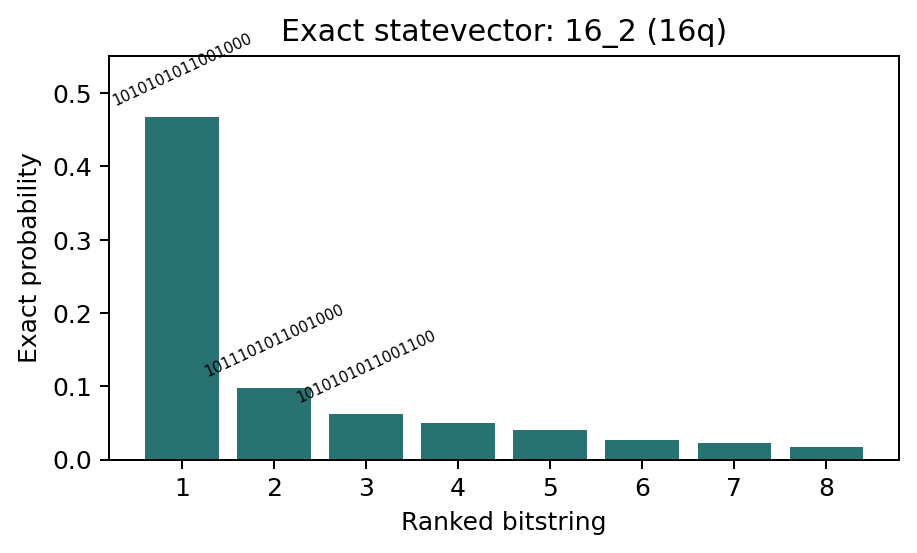
\includegraphics[width=\linewidth]{figures/appendix_exact/exact_16_2.png}
\caption*{\code{16\_2}: exact statevector top probabilities.}
\end{minipage}
\caption{Exact statevector top-k distributions.}
\end{figure}

\begin{figure}[H]
\centering
\begin{minipage}{0.48\linewidth}
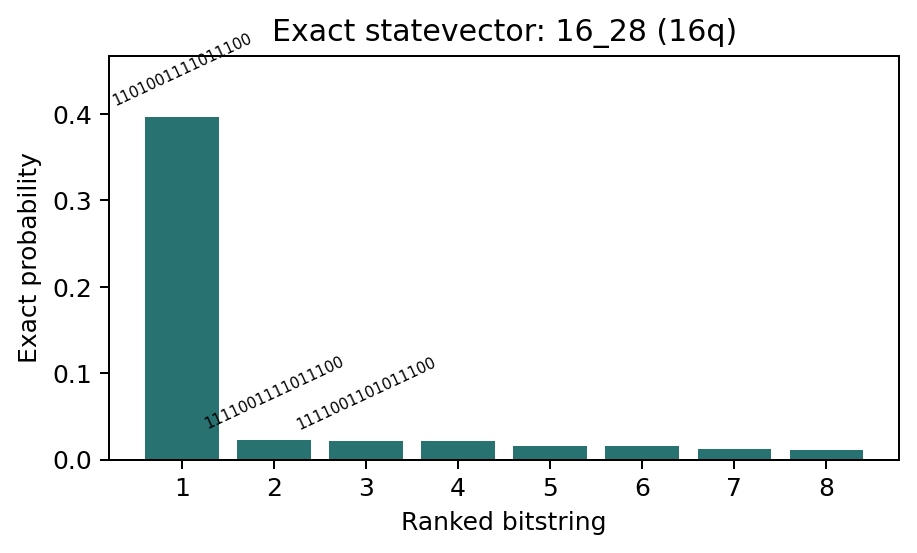
\includegraphics[width=\linewidth]{figures/appendix_exact/exact_16_28.png}
\caption*{\code{16\_28}: exact statevector top probabilities.}
\end{minipage}\hfill
\begin{minipage}{0.48\linewidth}
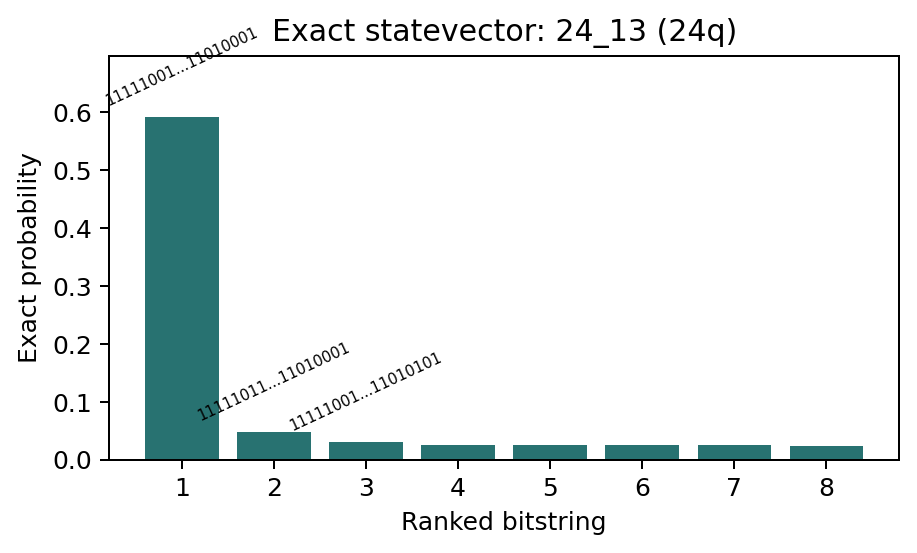
\includegraphics[width=\linewidth]{figures/appendix_exact/exact_24_13.png}
\caption*{\code{24\_13}: exact statevector top probabilities.}
\end{minipage}
\caption{Exact statevector top-k distributions.}
\end{figure}

\begin{figure}[H]
\centering
\begin{minipage}{0.48\linewidth}
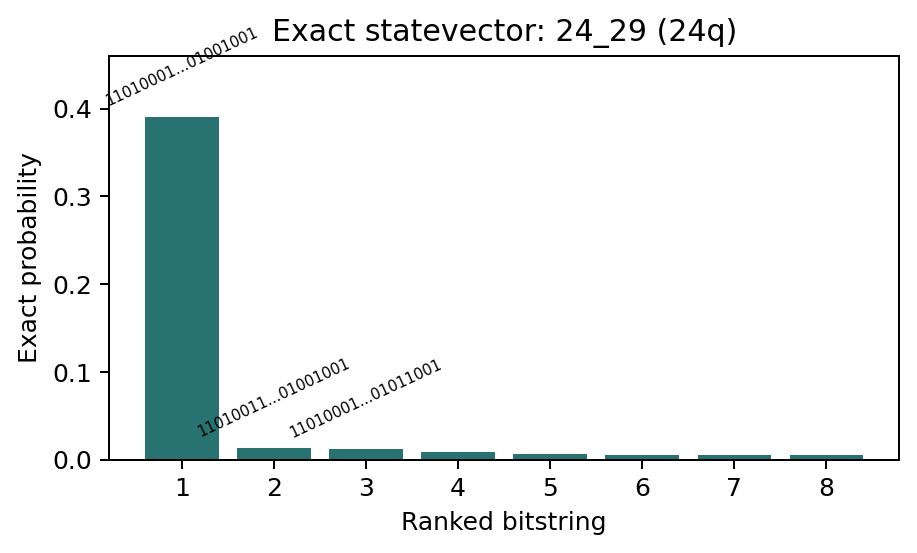
\includegraphics[width=\linewidth]{figures/appendix_exact/exact_24_29.png}
\caption*{\code{24\_29}: exact statevector top probabilities.}
\end{minipage}\hfill
\begin{minipage}{0.48\linewidth}
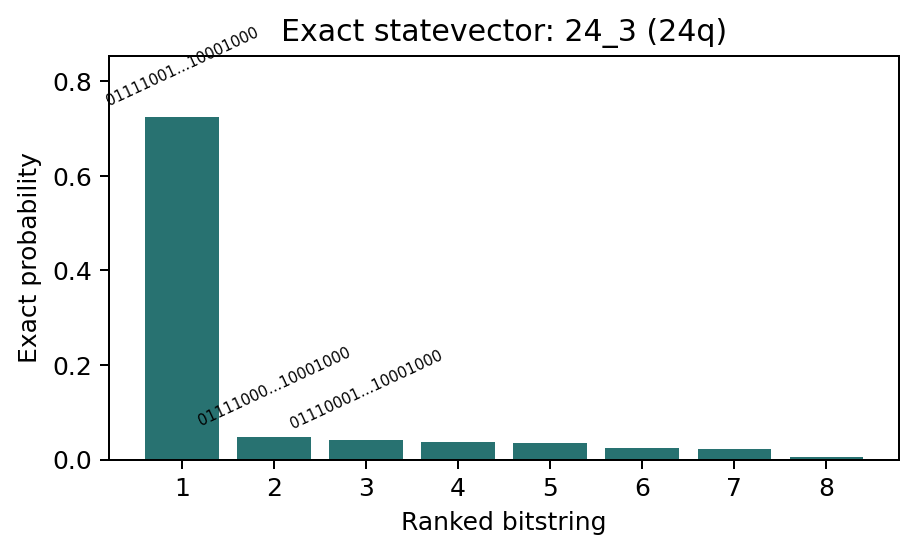
\includegraphics[width=\linewidth]{figures/appendix_exact/exact_24_3.png}
\caption*{\code{24\_3}: exact statevector top probabilities.}
\end{minipage}
\caption{Exact statevector top-k distributions.}
\end{figure}

\begin{figure}[H]
\centering
\begin{minipage}{0.48\linewidth}
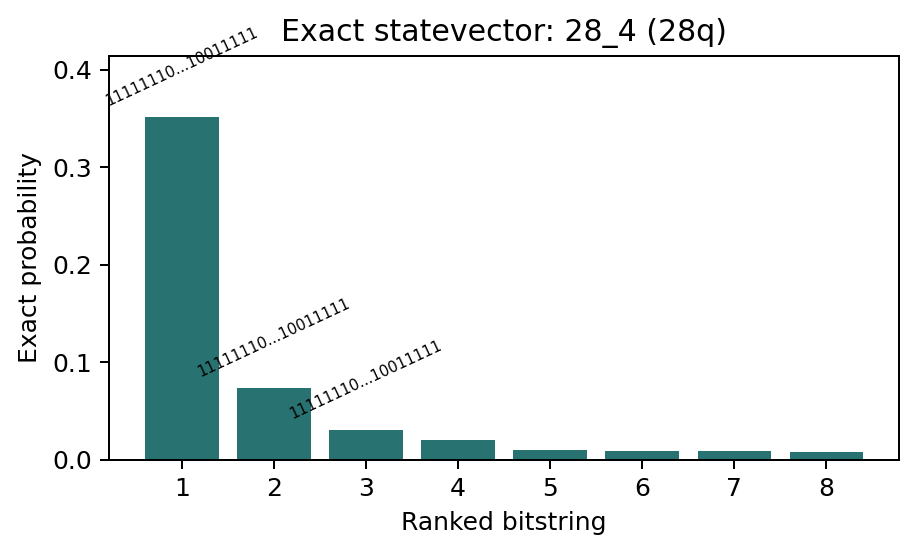
\includegraphics[width=\linewidth]{figures/appendix_exact/exact_28_4.png}
\caption*{\code{28\_4}: exact statevector top probabilities.}
\end{minipage}\hfill
\begin{minipage}{0.48\linewidth}
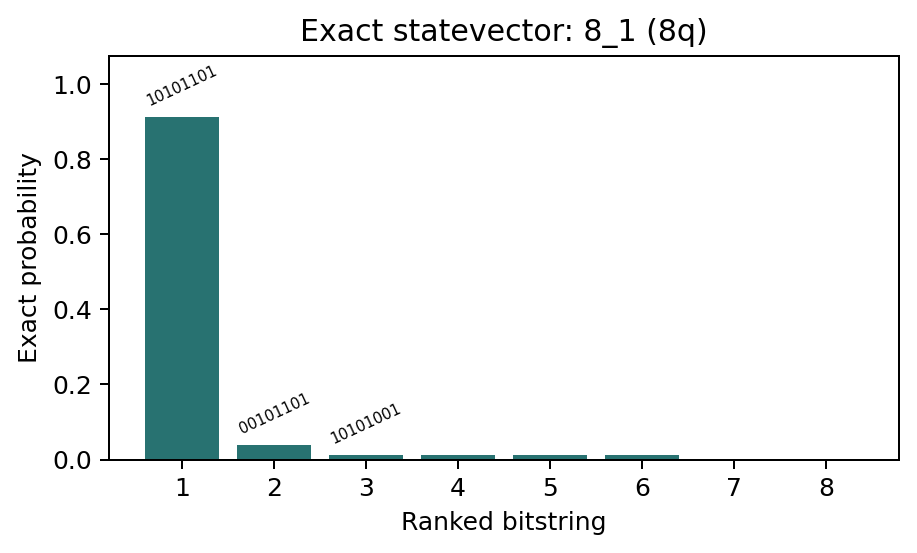
\includegraphics[width=\linewidth]{figures/appendix_exact/exact_8_1.png}
\caption*{\code{8\_1}: exact statevector top probabilities.}
\end{minipage}
\caption{Exact statevector top-k distributions.}
\end{figure}

\begin{figure}[H]
\centering
\begin{minipage}{0.48\linewidth}
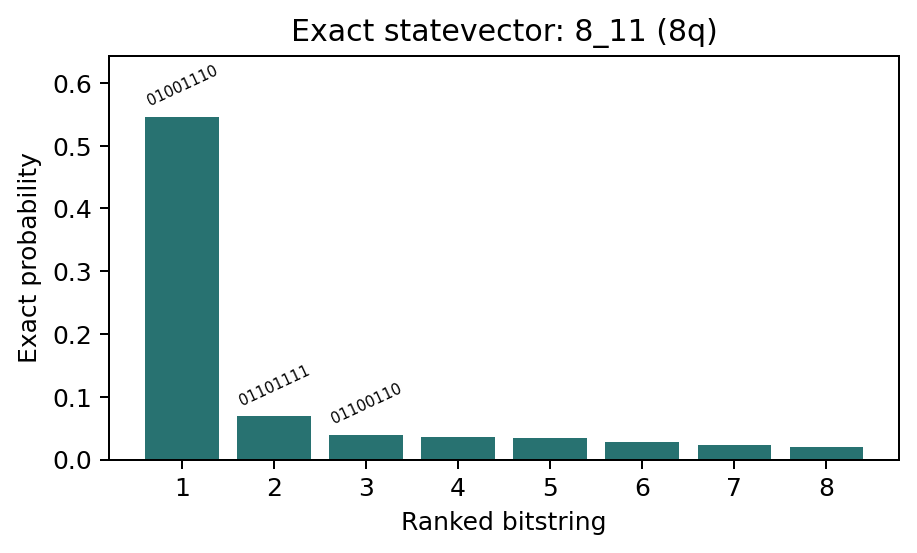
\includegraphics[width=\linewidth]{figures/appendix_exact/exact_8_11.png}
\caption*{\code{8\_11}: exact statevector top probabilities.}
\end{minipage}\hfill
\begin{minipage}{0.48\linewidth}
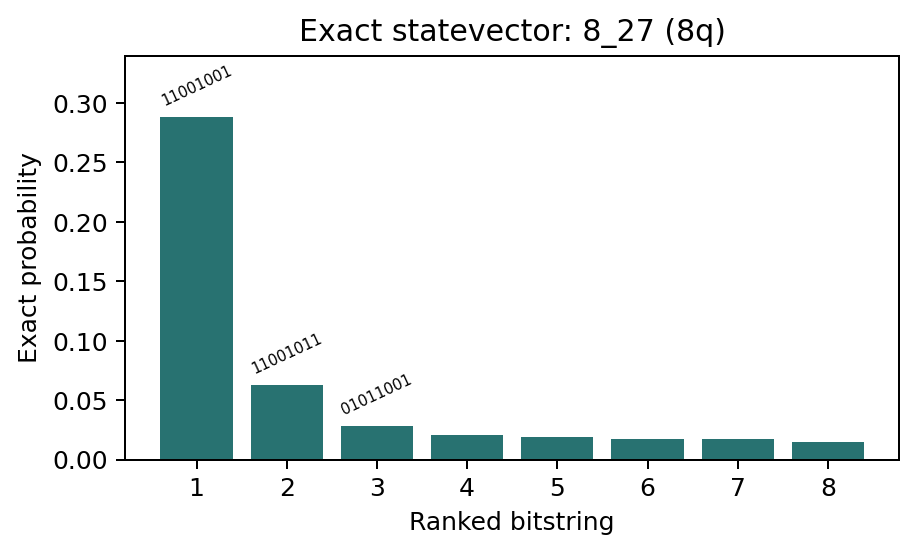
\includegraphics[width=\linewidth]{figures/appendix_exact/exact_8_27.png}
\caption*{\code{8\_27}: exact statevector top probabilities.}
\end{minipage}
\caption{Exact statevector top-k distributions.}
\end{figure}

\subsection{Requested Statevector/MPS Runs: IDs 11, 26, 34, 41, 49}
Only \code{8\_11} was small enough for exact statevector in this requested set. The other statevector entries were skipped by design; the useful distributions are the MPS sample-count plots below.
\begin{figure}[H]
\centering
\begin{minipage}{0.48\linewidth}
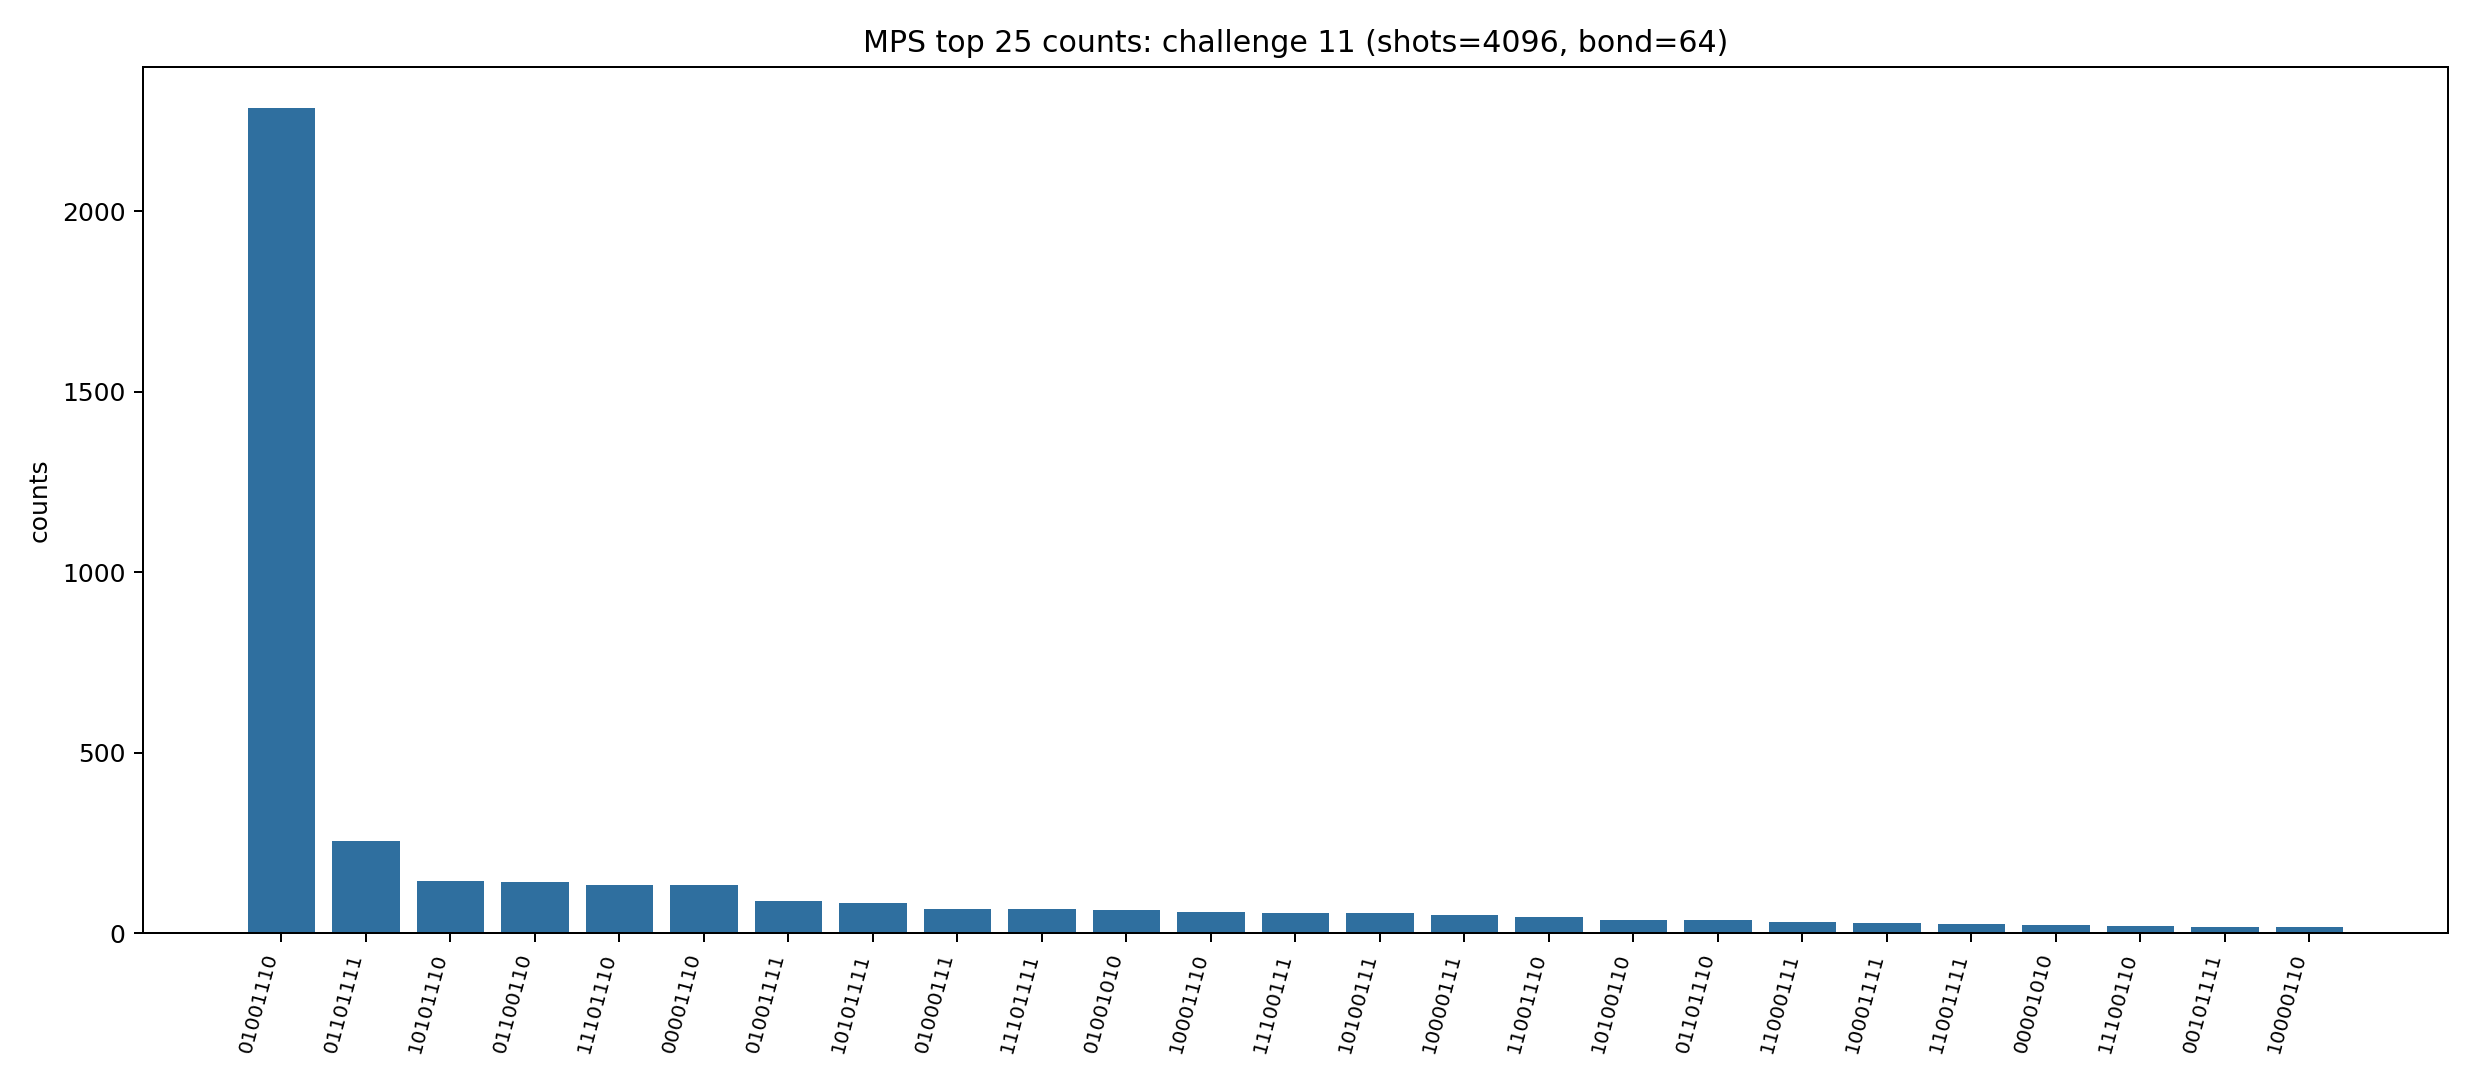
\includegraphics[width=\linewidth]{figures/mps_8_11.png}
\caption*{\code{8\_11}: MPS sample distribution; matches exact.}
\end{minipage}\hfill
\begin{minipage}{0.48\linewidth}
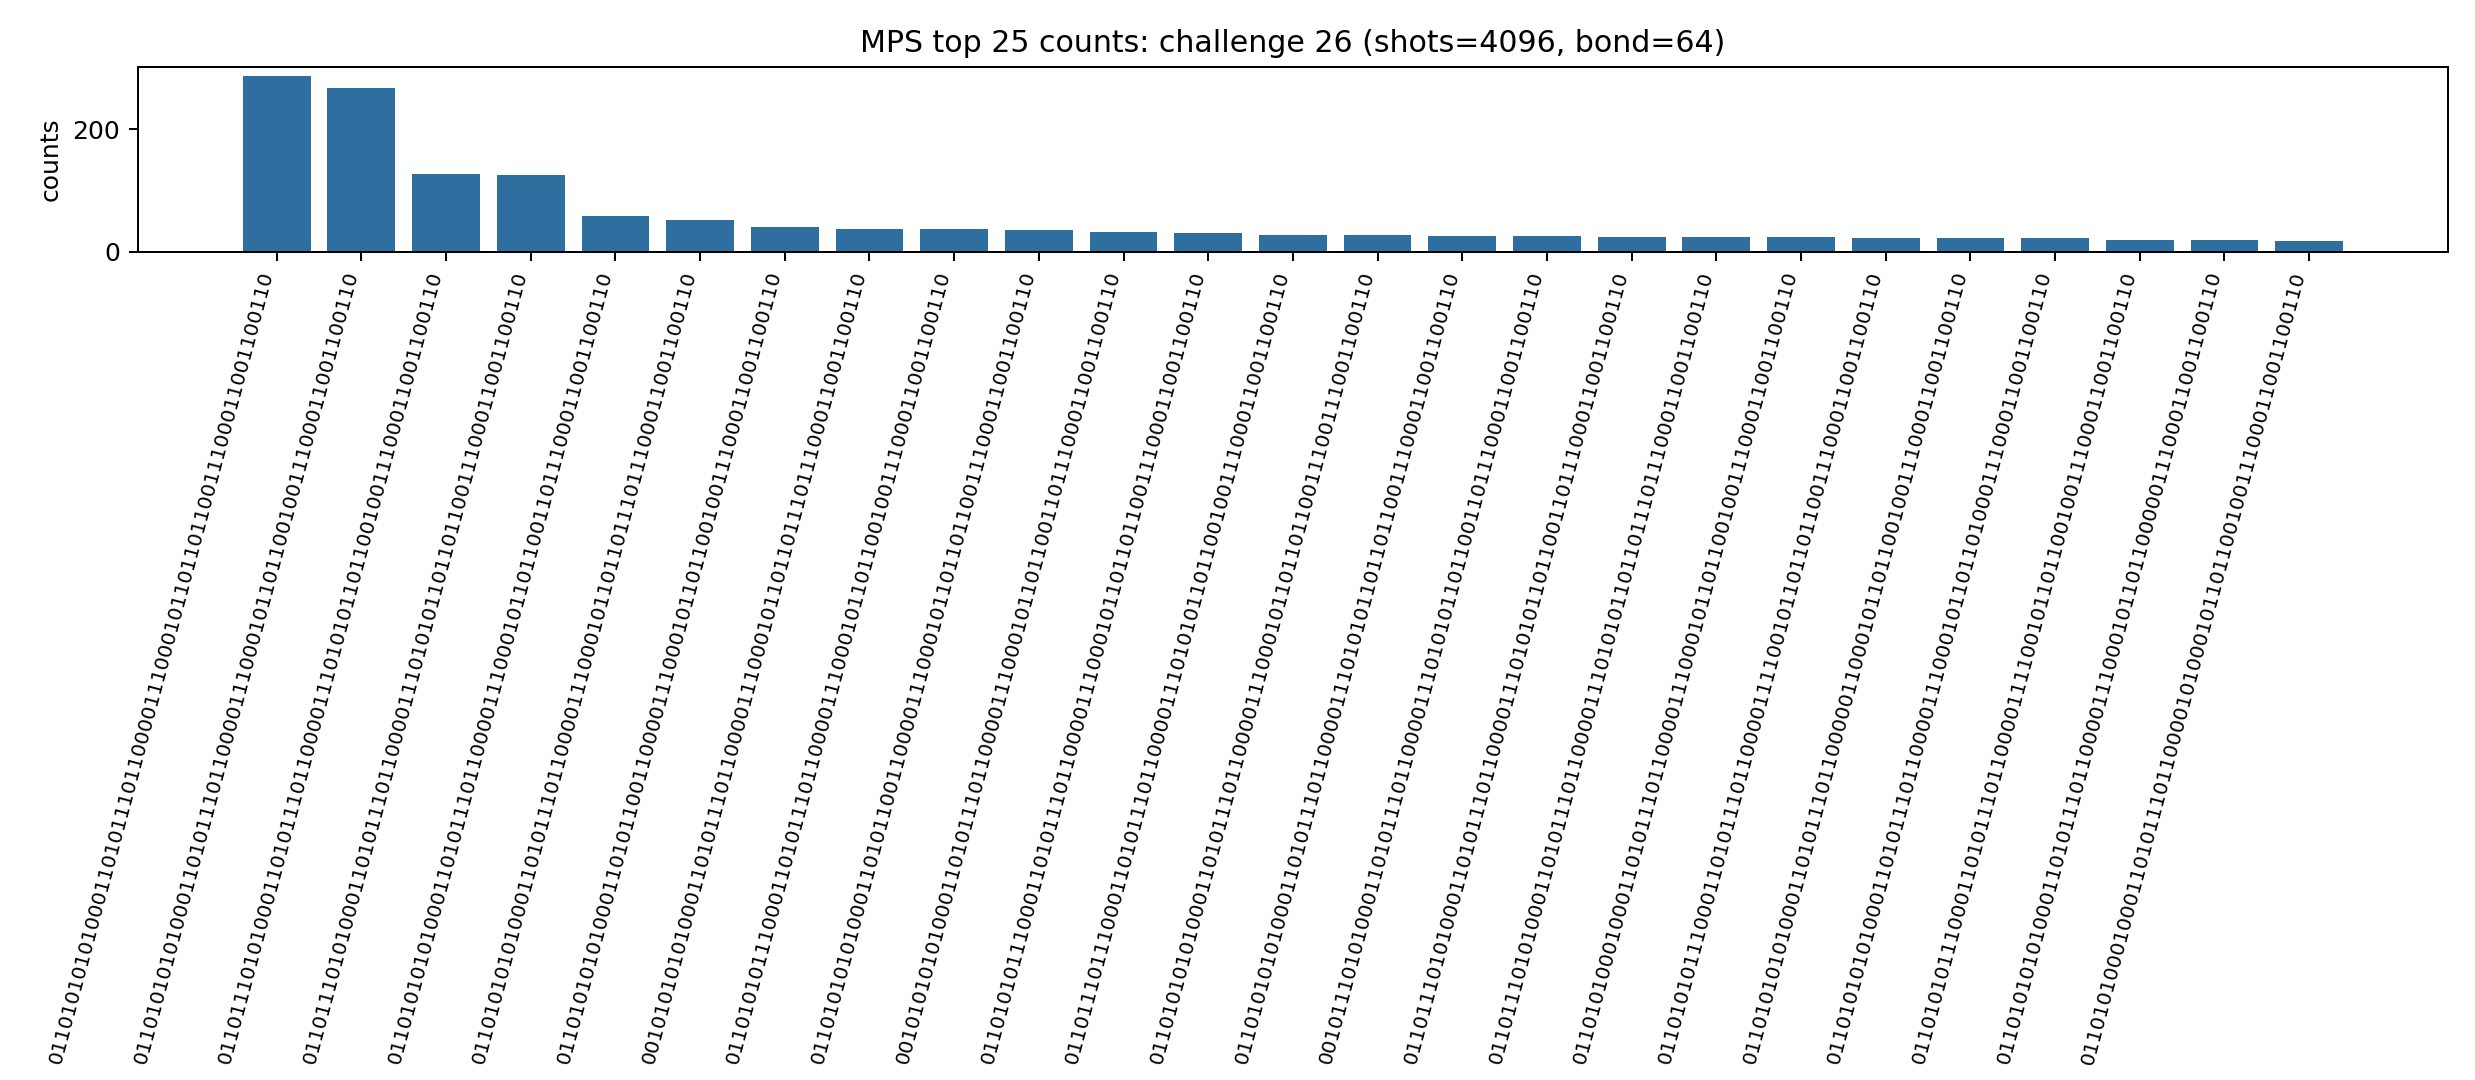
\includegraphics[width=\linewidth]{figures/mps_64_26.png}
\caption*{\code{64\_26}: MPS sample distribution; repeated top sample, medium confidence.}
\end{minipage}
\caption{Requested MPS sample-count distributions.}
\end{figure}

\begin{figure}[H]
\centering
\begin{minipage}{0.48\linewidth}
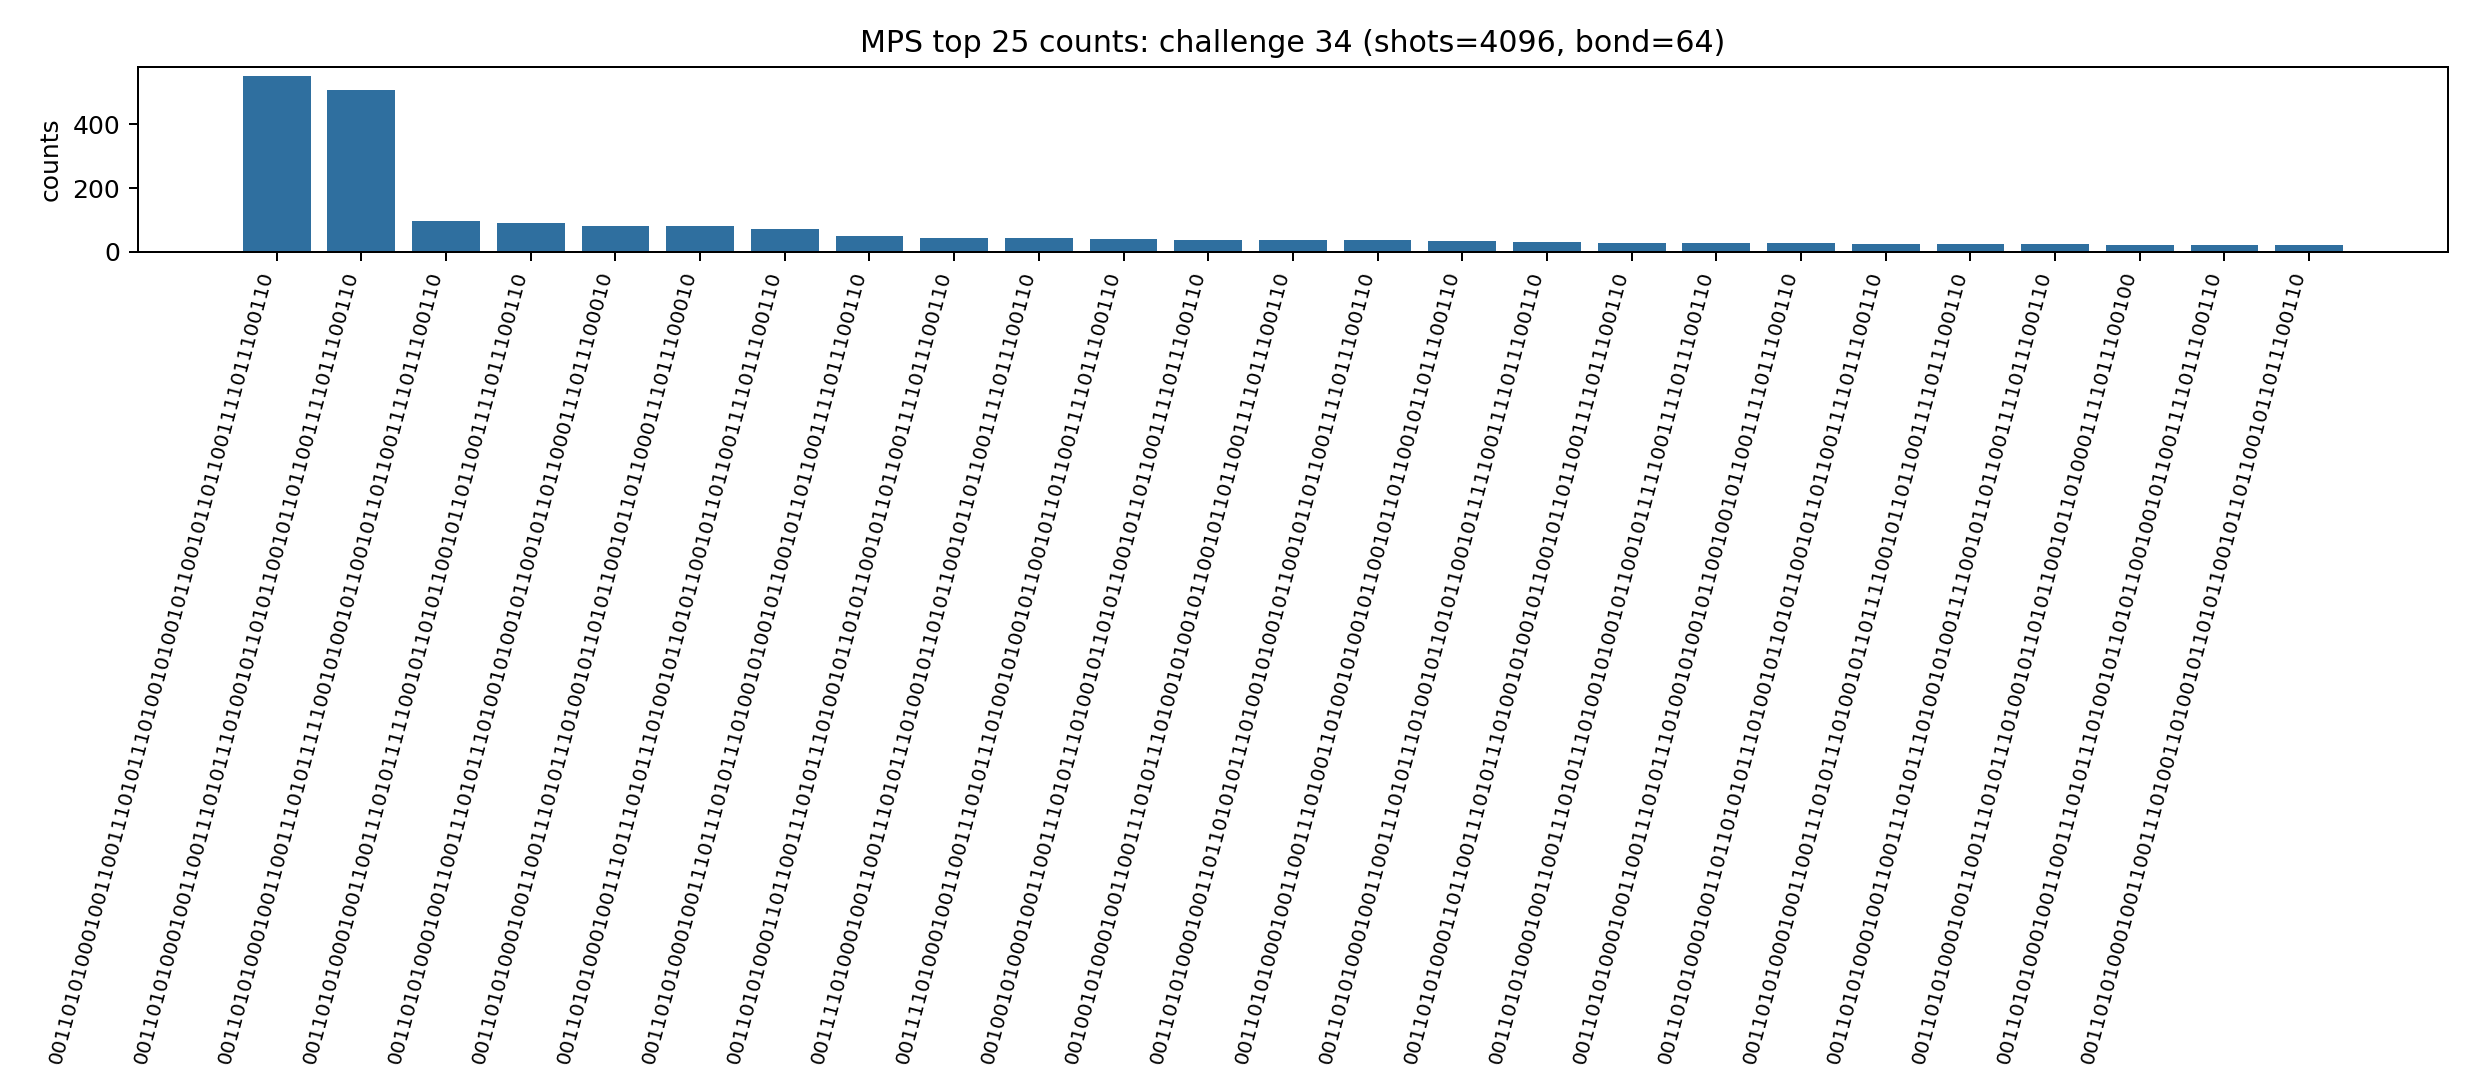
\includegraphics[width=\linewidth]{figures/mps_64_34.png}
\caption*{\code{64\_34}: MPS sample distribution; repeated top sample, medium confidence.}
\end{minipage}\hfill
\begin{minipage}{0.48\linewidth}
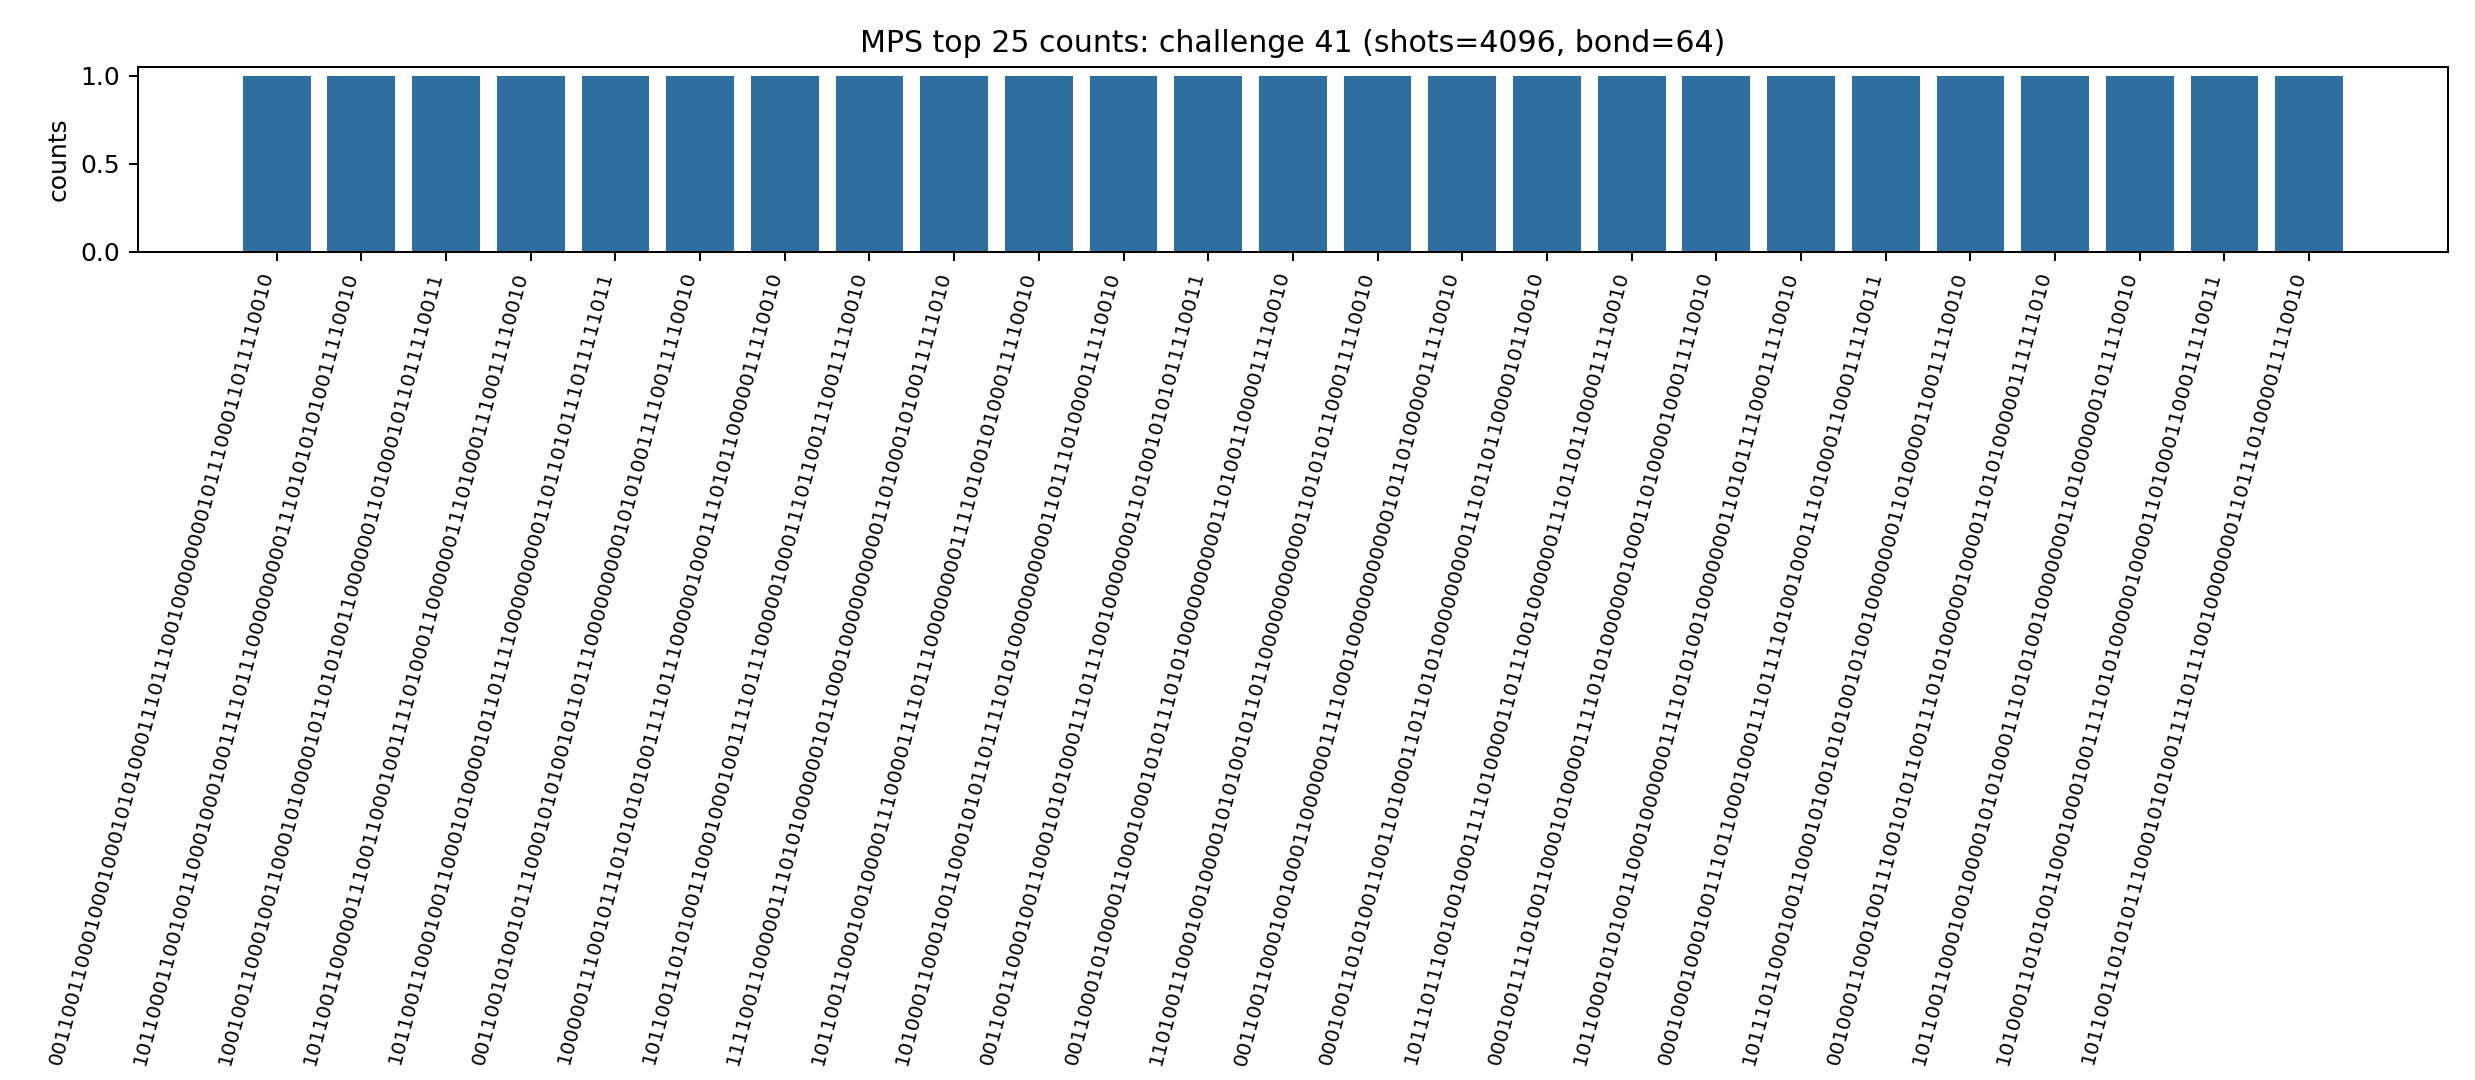
\includegraphics[width=\linewidth]{figures/mps_64_41.png}
\caption*{\code{64\_41}: MPS sample distribution; all-unique behavior, low confidence.}
\end{minipage}
\caption{Requested MPS sample-count distributions.}
\end{figure}

\begin{figure}[H]
\centering
\begin{minipage}{0.48\linewidth}
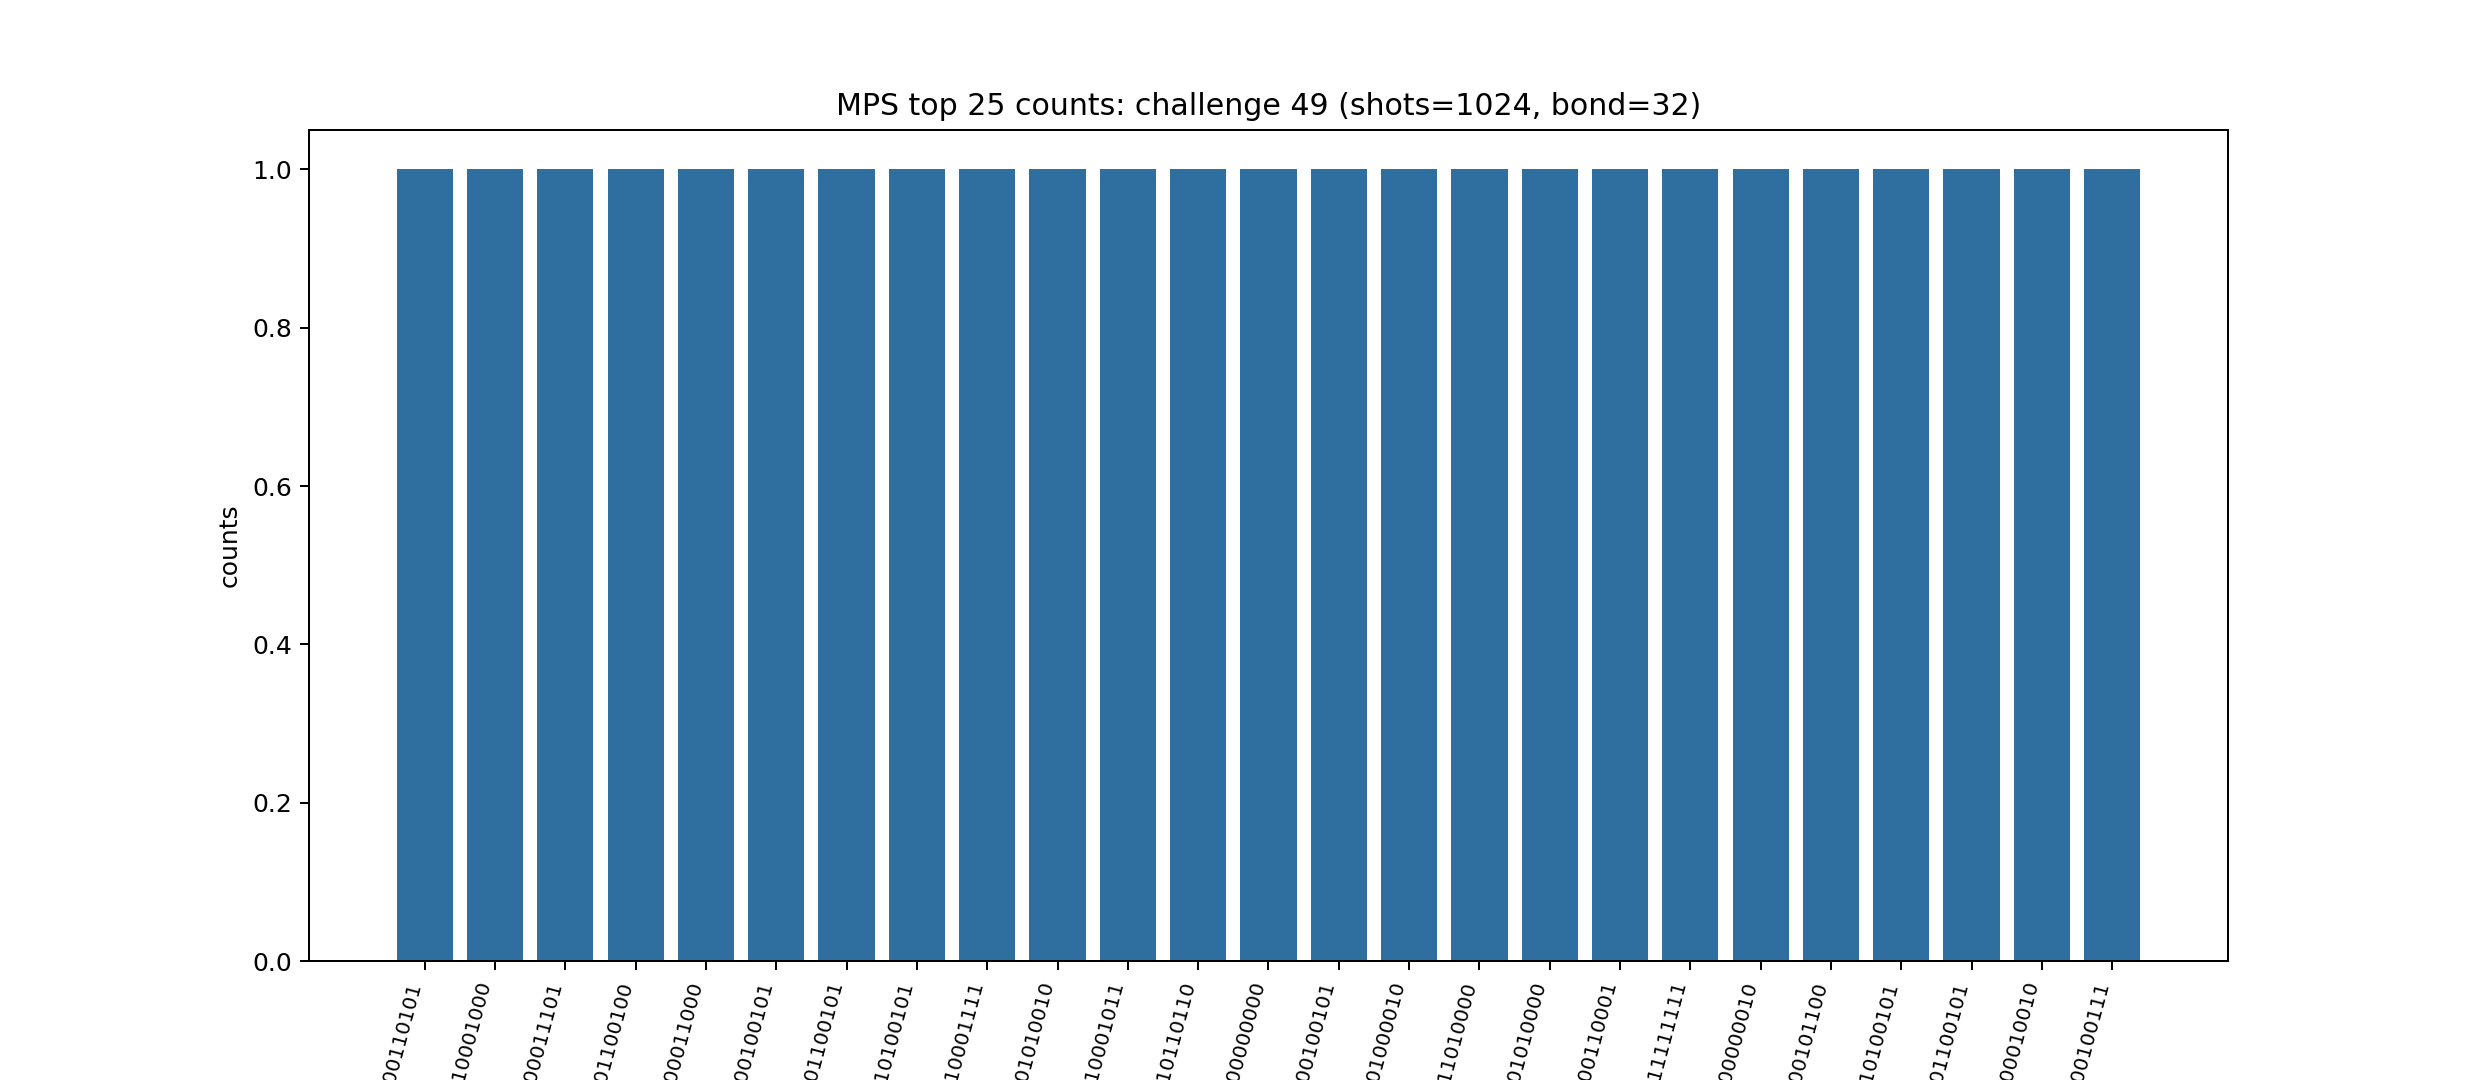
\includegraphics[width=\linewidth]{figures/mps_104_49.png}
\caption*{\code{104\_49}: MPS sample distribution; all-unique behavior, low confidence.}
\end{minipage}
\caption{Requested MPS sample-count distributions.}
\end{figure}

\subsection{MPS Distillation Aggregate Distributions}
These plots aggregate the top samples reported by the six pilot trials per circuit. Stable circuits have one repeated winner; unstable circuits have nearly flat counts.
\begin{figure}[H]
\centering
\begin{minipage}{0.48\linewidth}
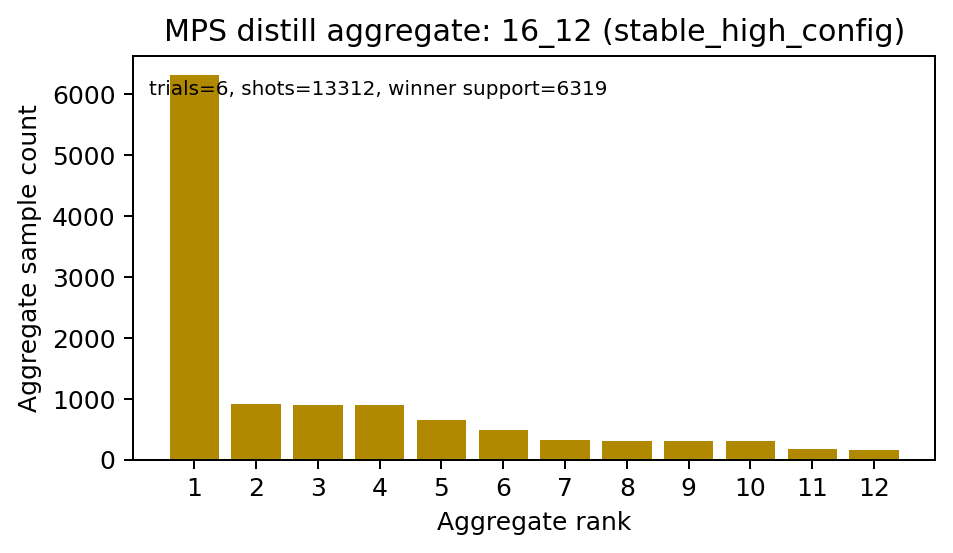
\includegraphics[width=\linewidth]{figures/appendix_mps_distill/mps_distill_16_12.png}
\caption*{\code{16\_12}: aggregate MPS-distillation counts.}
\end{minipage}\hfill
\begin{minipage}{0.48\linewidth}
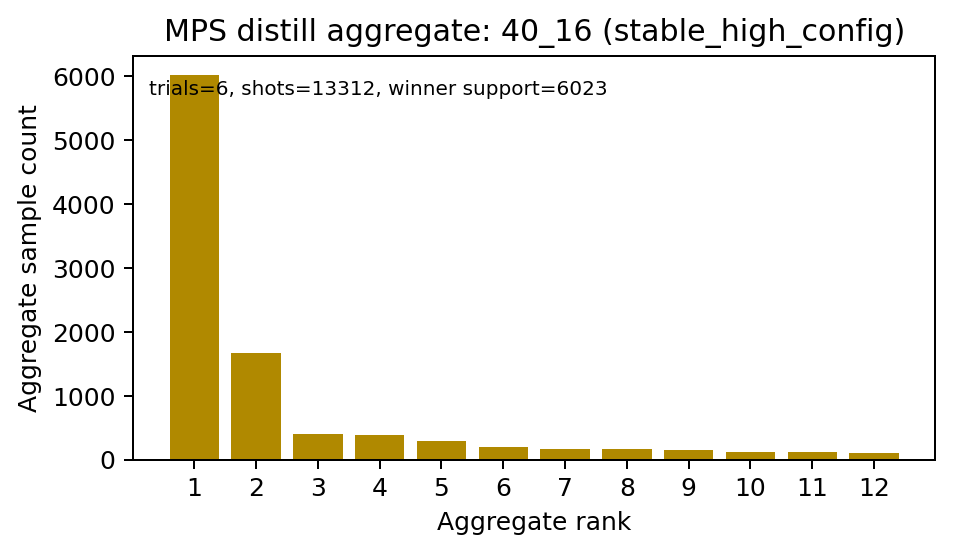
\includegraphics[width=\linewidth]{figures/appendix_mps_distill/mps_distill_40_16.png}
\caption*{\code{40\_16}: aggregate MPS-distillation counts.}
\end{minipage}
\caption{MPS-distillation aggregate distributions.}
\end{figure}

\begin{figure}[H]
\centering
\begin{minipage}{0.48\linewidth}
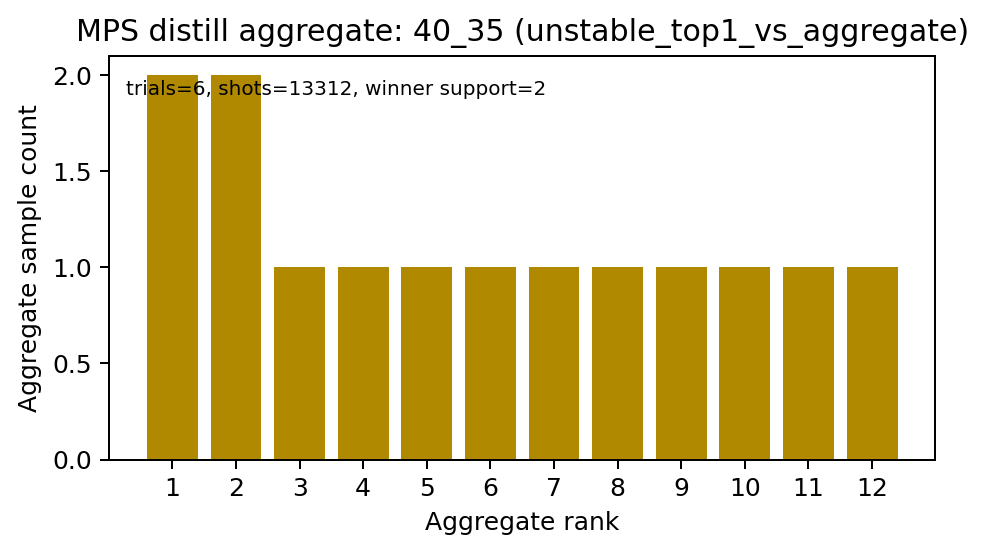
\includegraphics[width=\linewidth]{figures/appendix_mps_distill/mps_distill_40_35.png}
\caption*{\code{40\_35}: aggregate MPS-distillation counts.}
\end{minipage}\hfill
\begin{minipage}{0.48\linewidth}
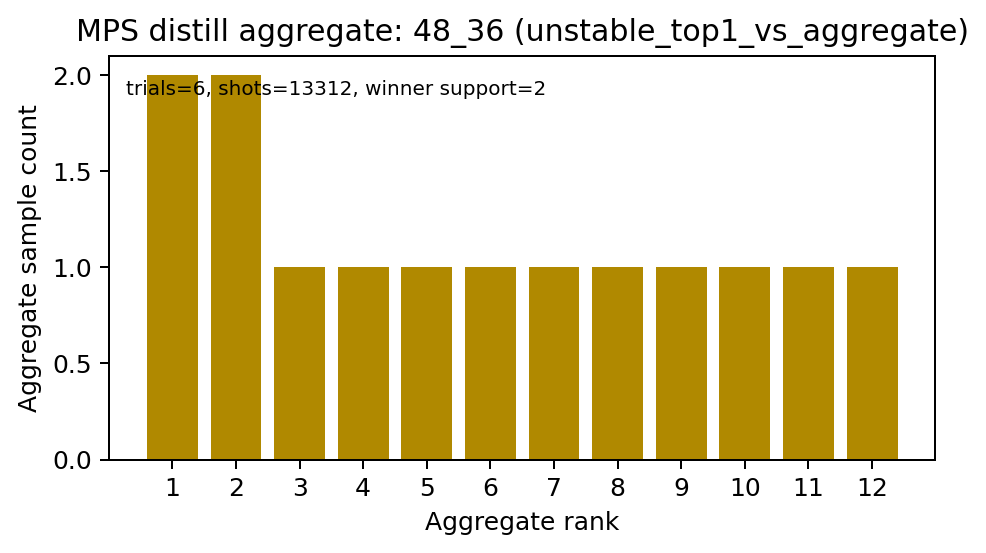
\includegraphics[width=\linewidth]{figures/appendix_mps_distill/mps_distill_48_36.png}
\caption*{\code{48\_36}: aggregate MPS-distillation counts.}
\end{minipage}
\caption{MPS-distillation aggregate distributions.}
\end{figure}

\begin{figure}[H]
\centering
\begin{minipage}{0.48\linewidth}
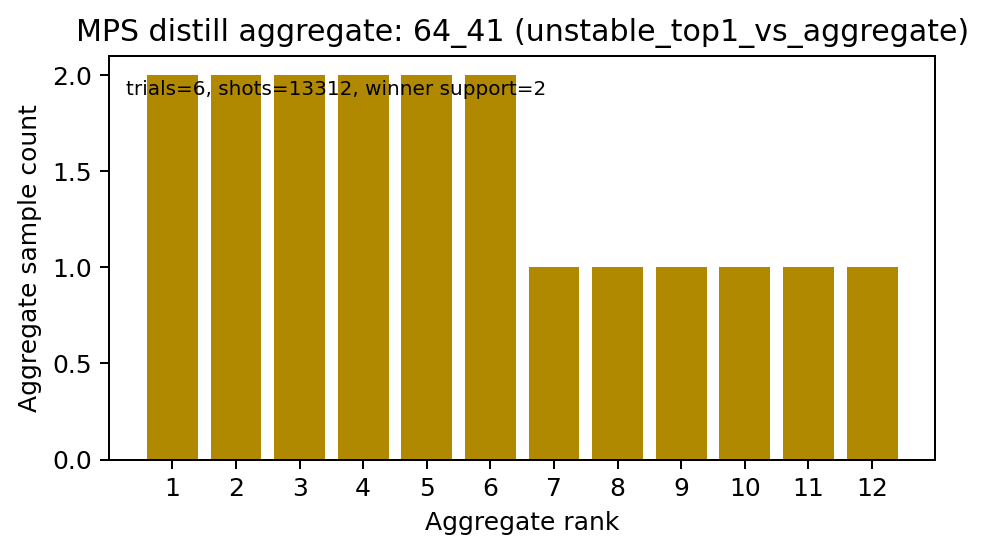
\includegraphics[width=\linewidth]{figures/appendix_mps_distill/mps_distill_64_41.png}
\caption*{\code{64\_41}: aggregate MPS-distillation counts.}
\end{minipage}\hfill
\begin{minipage}{0.48\linewidth}
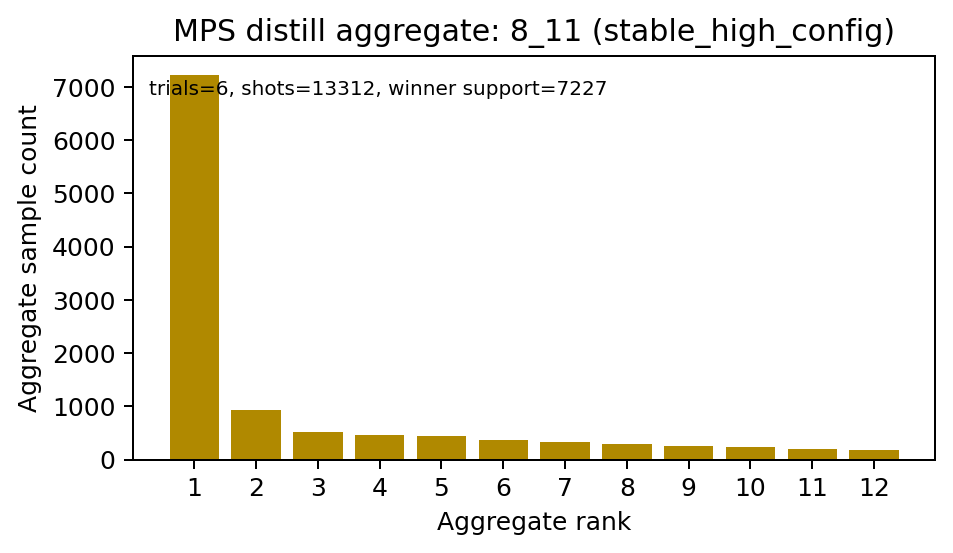
\includegraphics[width=\linewidth]{figures/appendix_mps_distill/mps_distill_8_11.png}
\caption*{\code{8\_11}: aggregate MPS-distillation counts.}
\end{minipage}
\caption{MPS-distillation aggregate distributions.}
\end{figure}

\subsection{\code{peaked-circuit-simulation} Marginal Distributions}
The following plots show one-qubit $P(1)$ marginals from the MPO/unswapping pipeline. They are useful as bit-level diagnostics, but the \code{24\_13} exact check shows why marginal thresholding alone is not submission-safe.
\begin{figure}[H]
\centering
\begin{minipage}{0.48\linewidth}
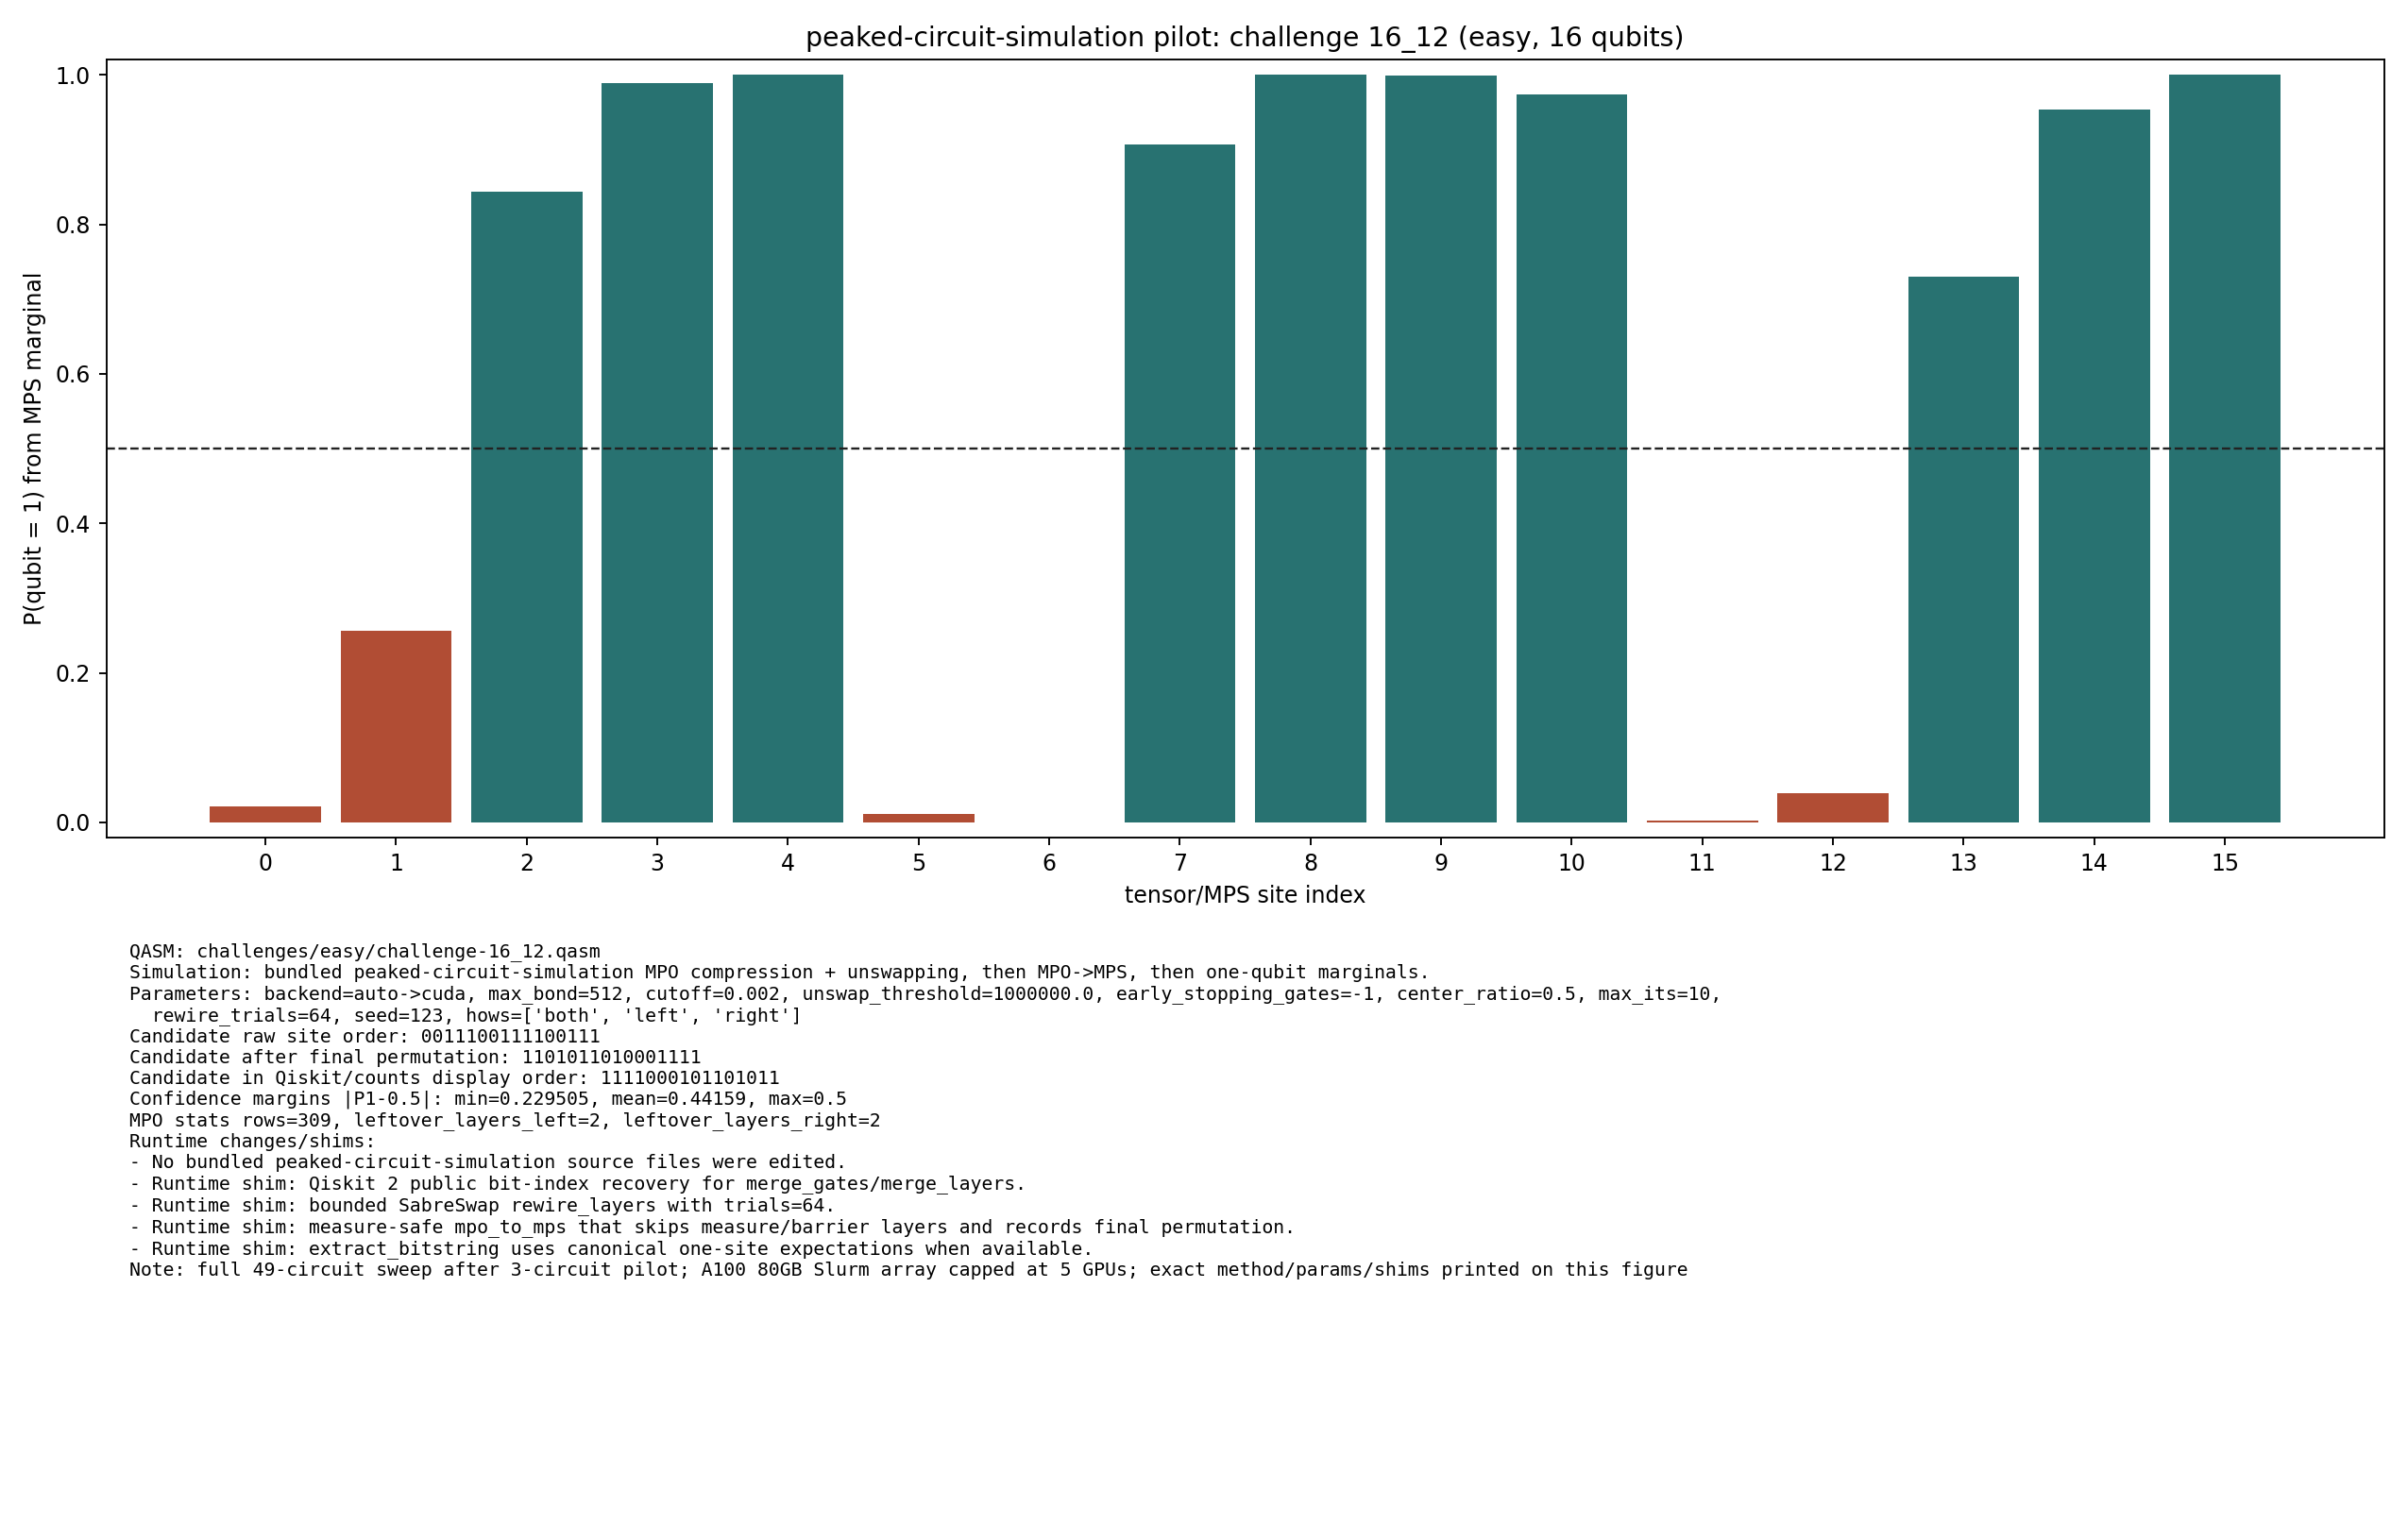
\includegraphics[width=\linewidth]{figures/appendix_peaked_16_12.png}
\caption*{\code{16\_12}: per-qubit marginal distribution.}
\end{minipage}\hfill
\begin{minipage}{0.48\linewidth}
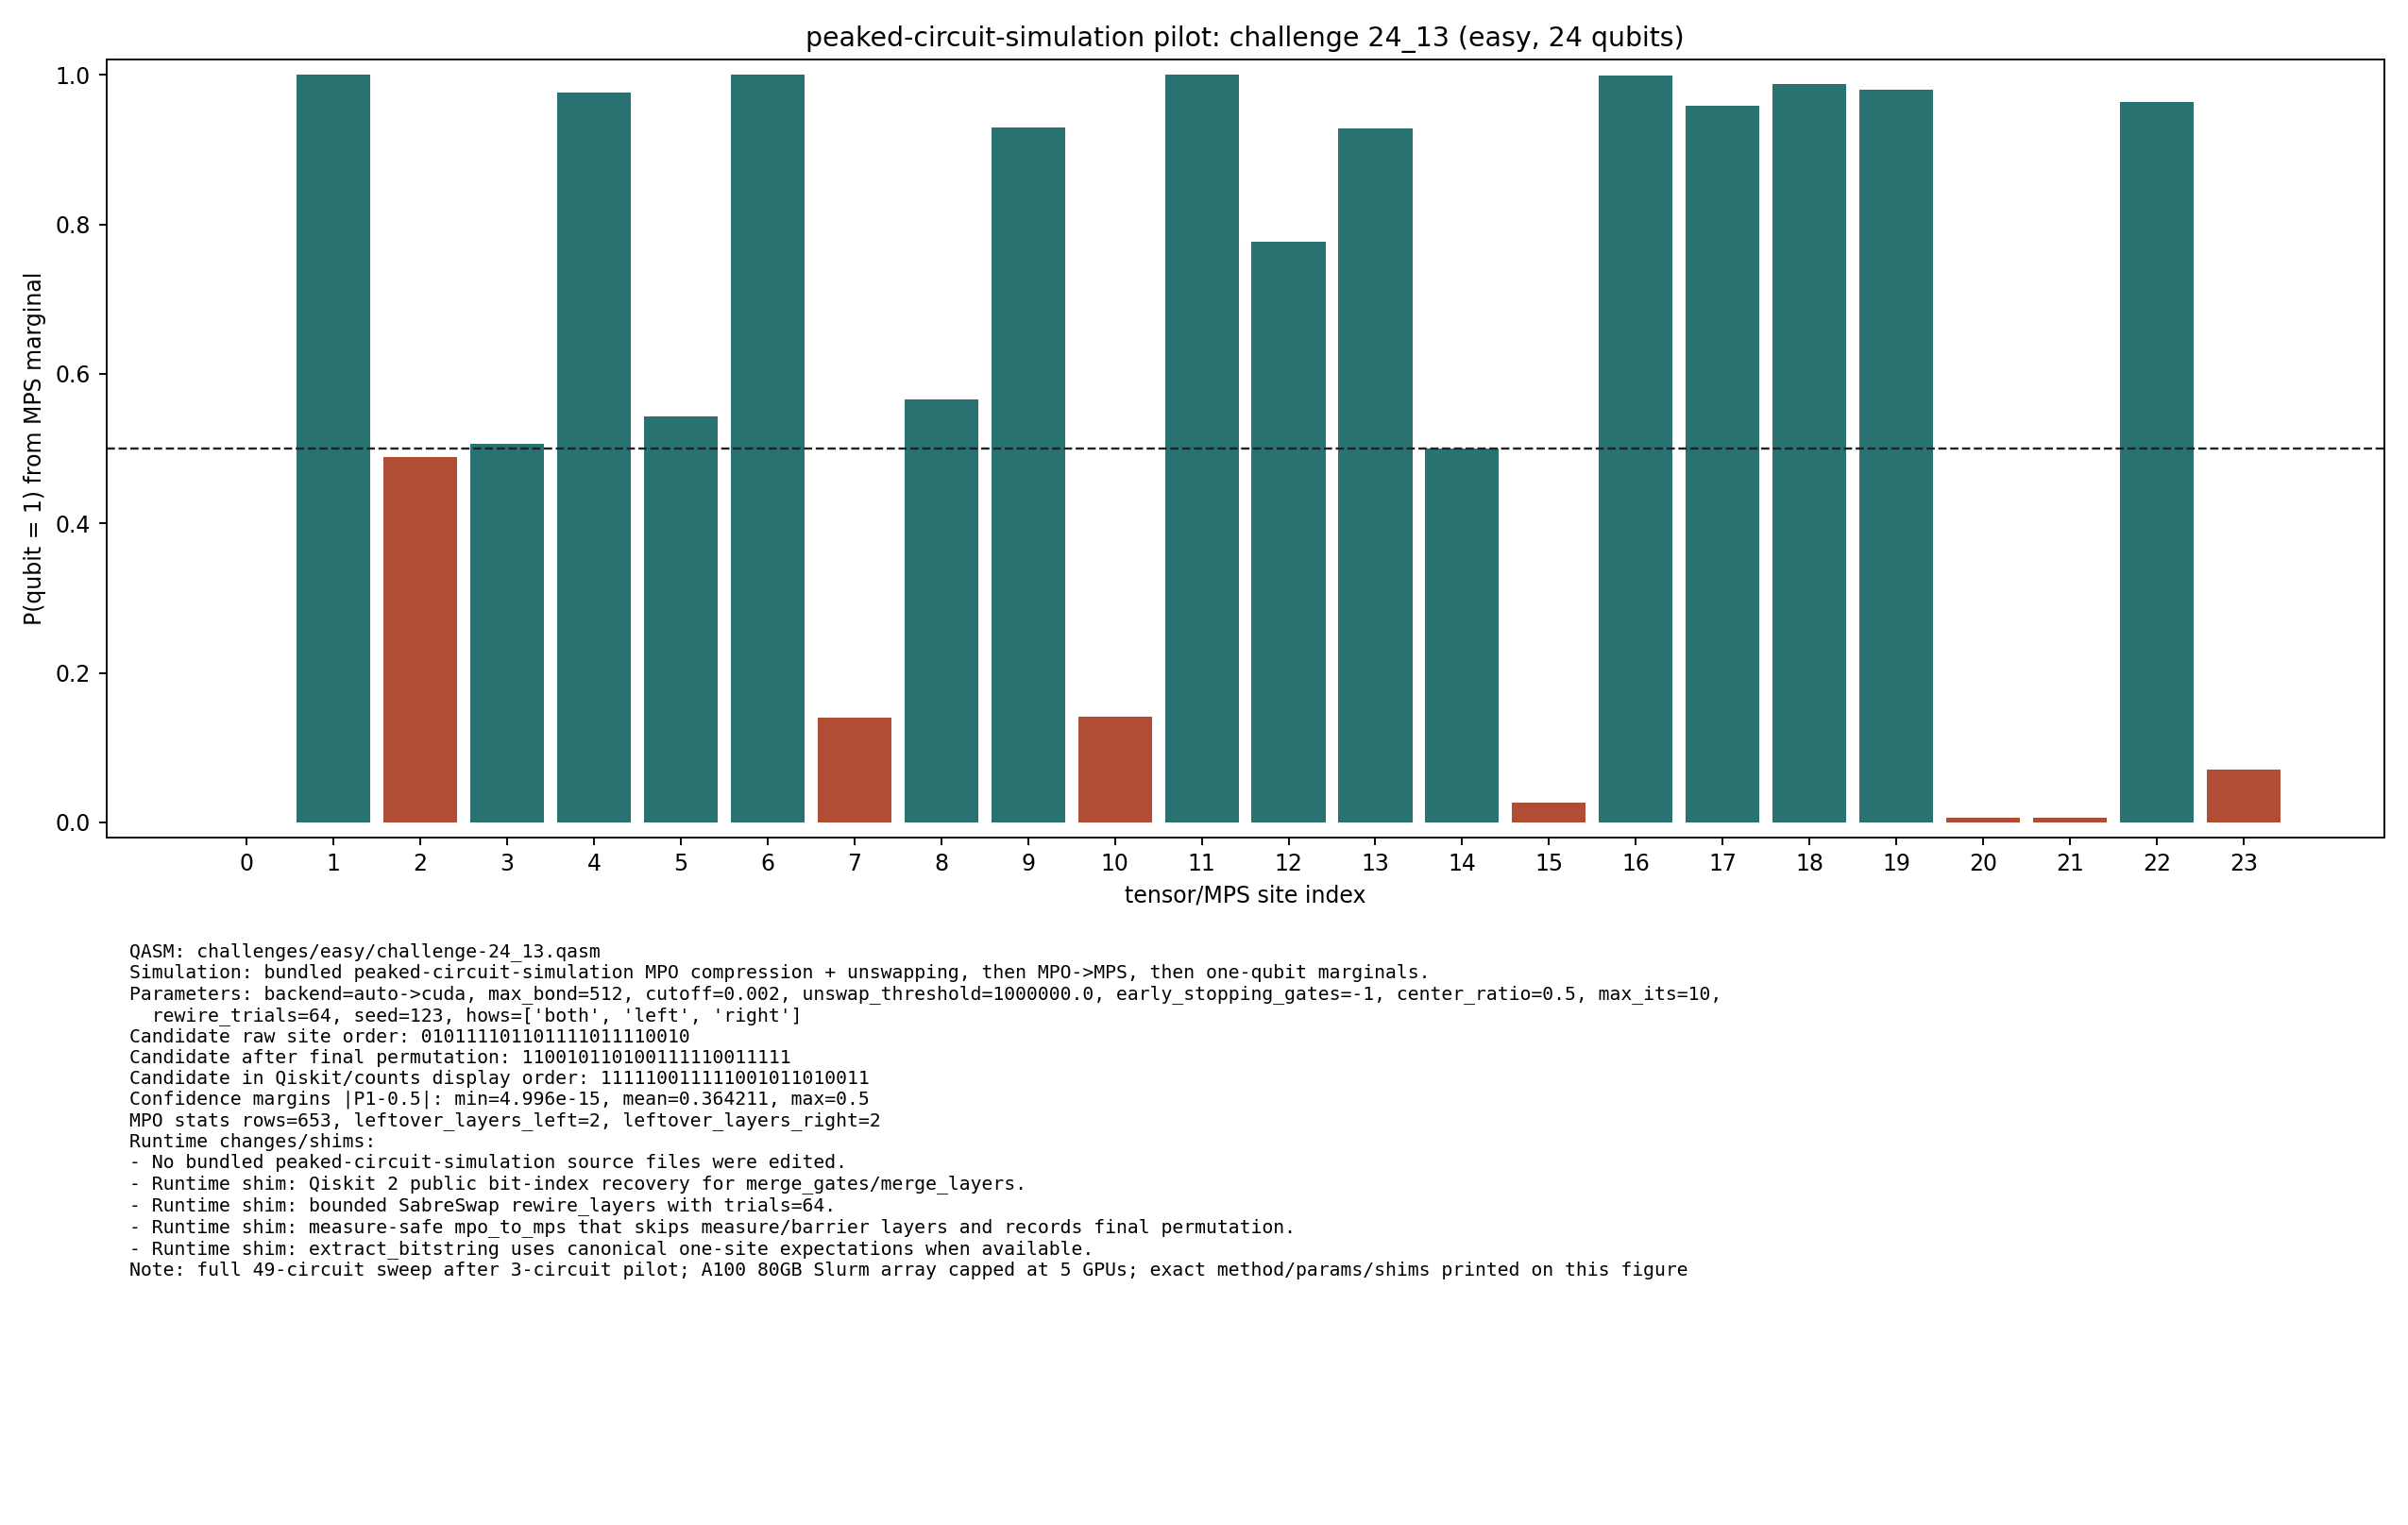
\includegraphics[width=\linewidth]{figures/appendix_peaked_24_13.png}
\caption*{\code{24\_13}: per-qubit marginal distribution.}
\end{minipage}
\caption{\code{peaked-circuit-simulation} marginal distributions.}
\end{figure}

\begin{figure}[H]
\centering
\begin{minipage}{0.48\linewidth}
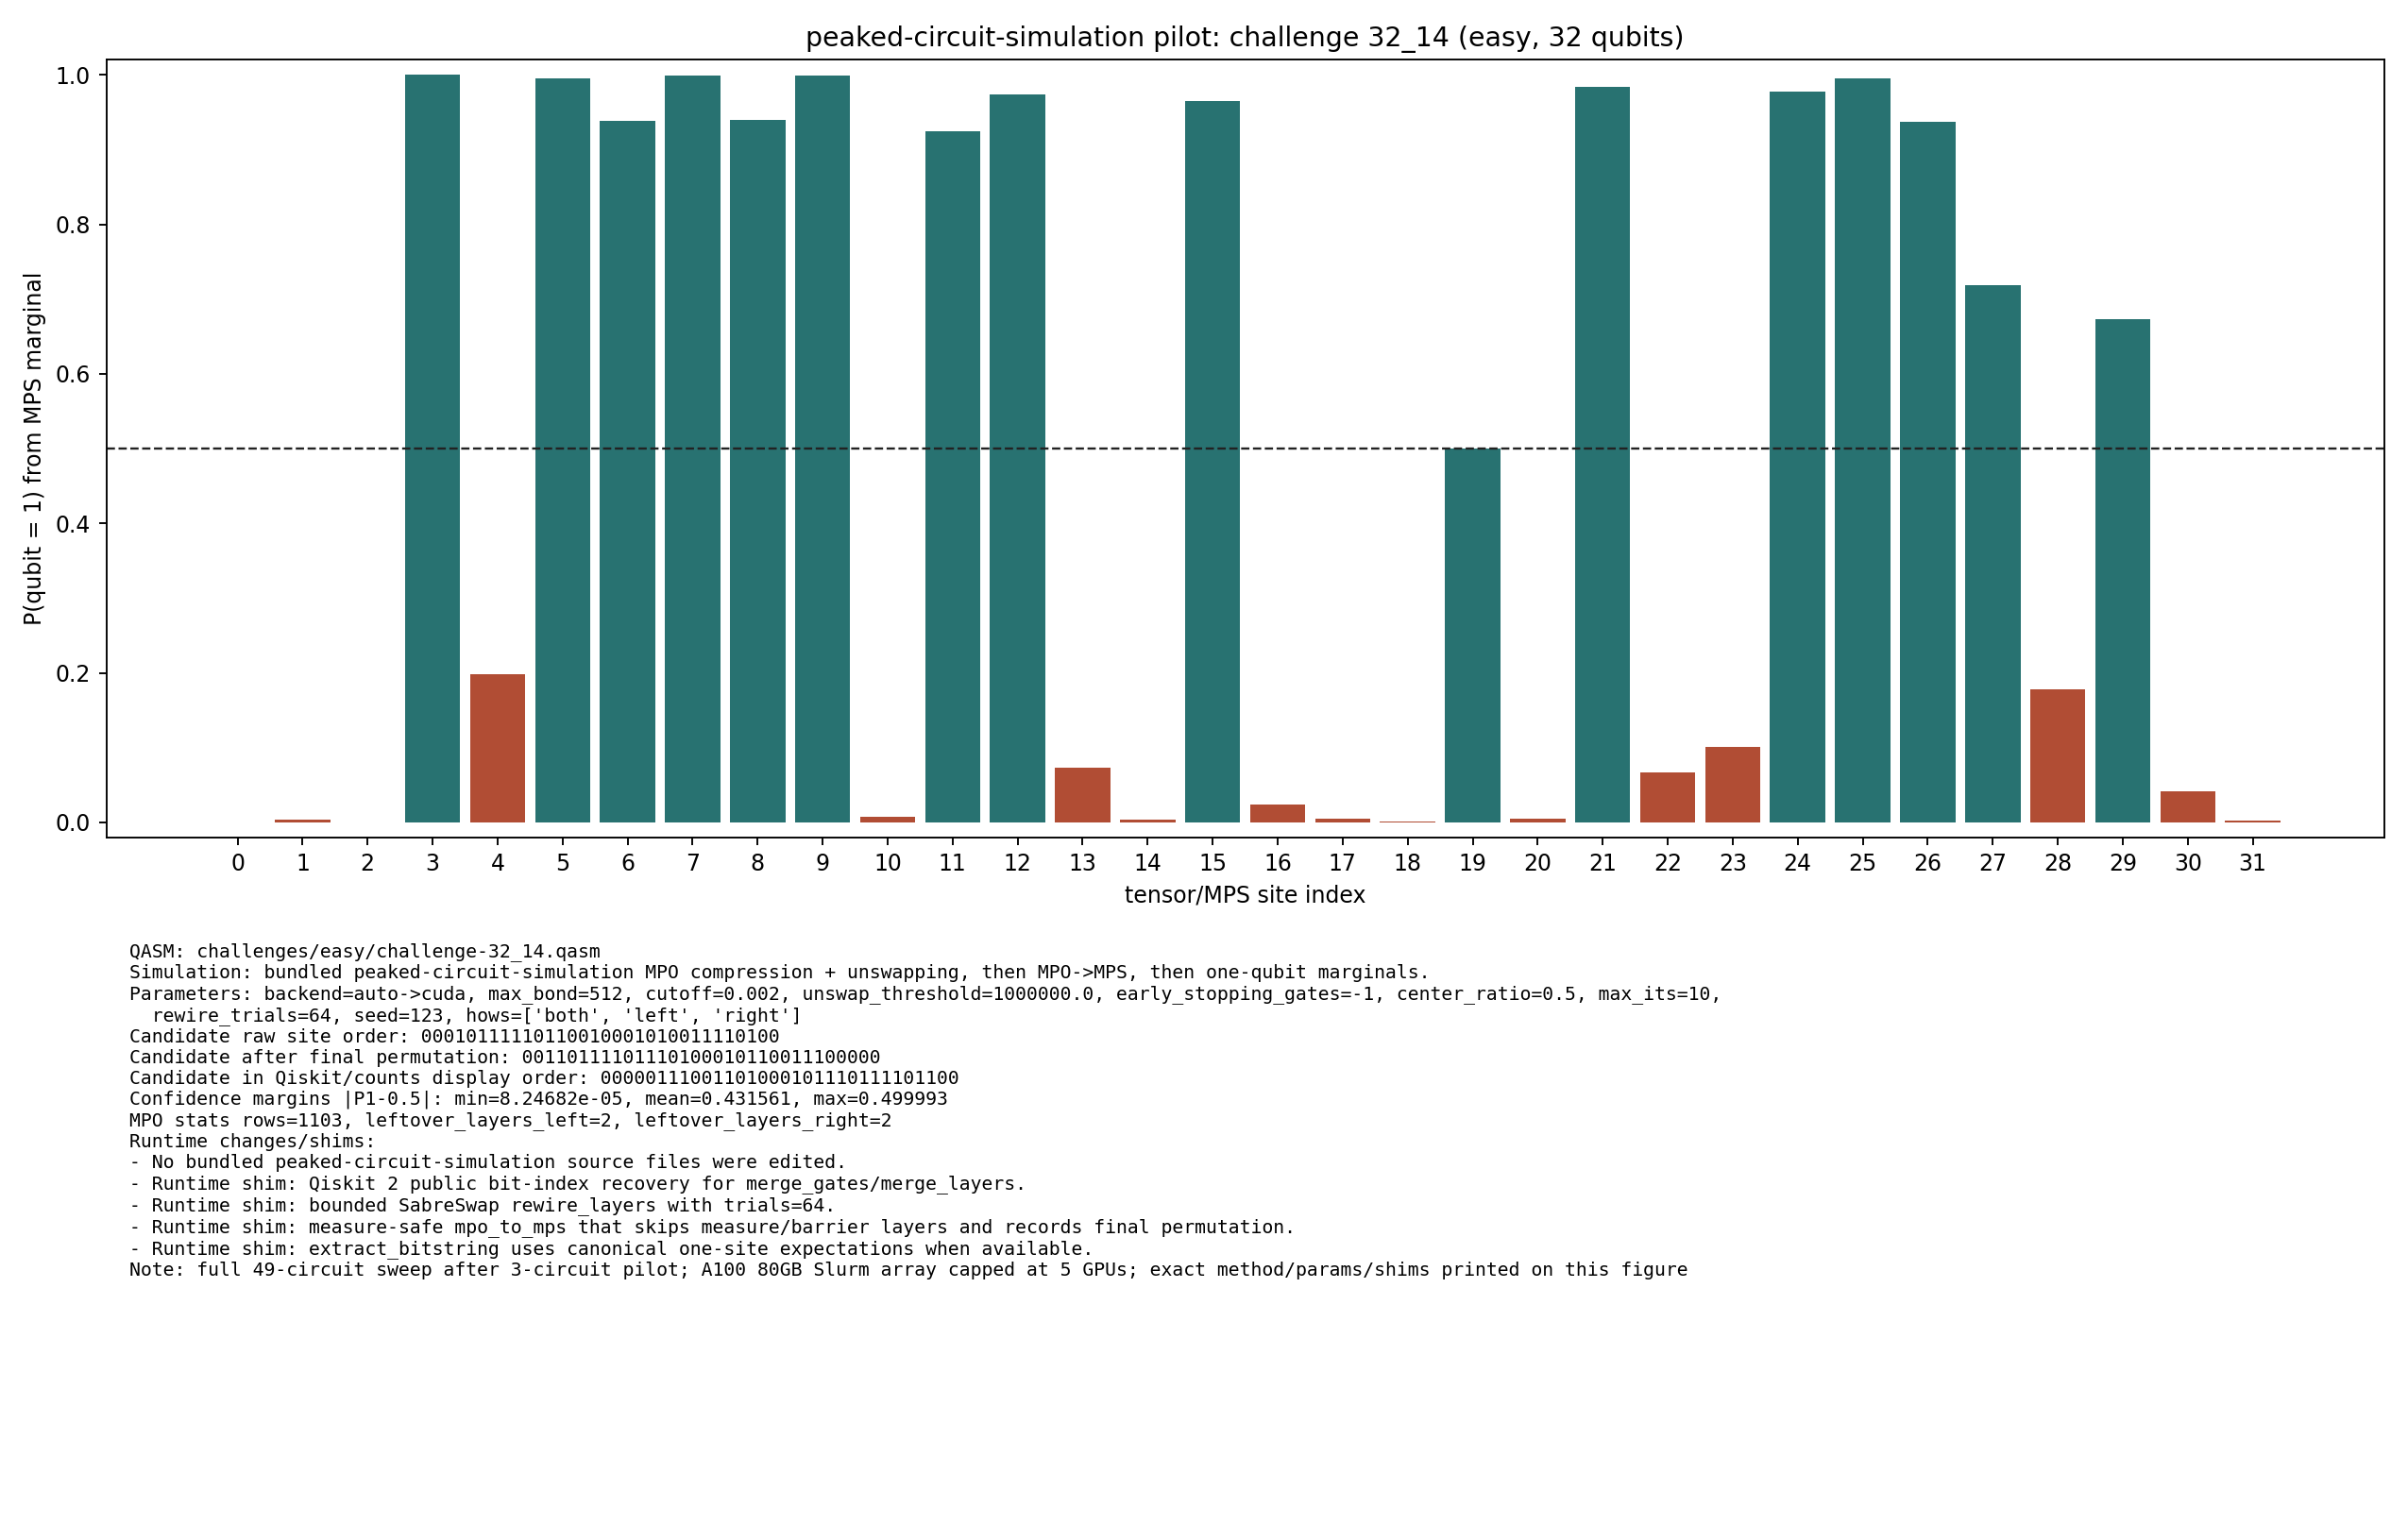
\includegraphics[width=\linewidth]{figures/appendix_peaked_32_14.png}
\caption*{\code{32\_14}: per-qubit marginal distribution.}
\end{minipage}\hfill
\begin{minipage}{0.48\linewidth}
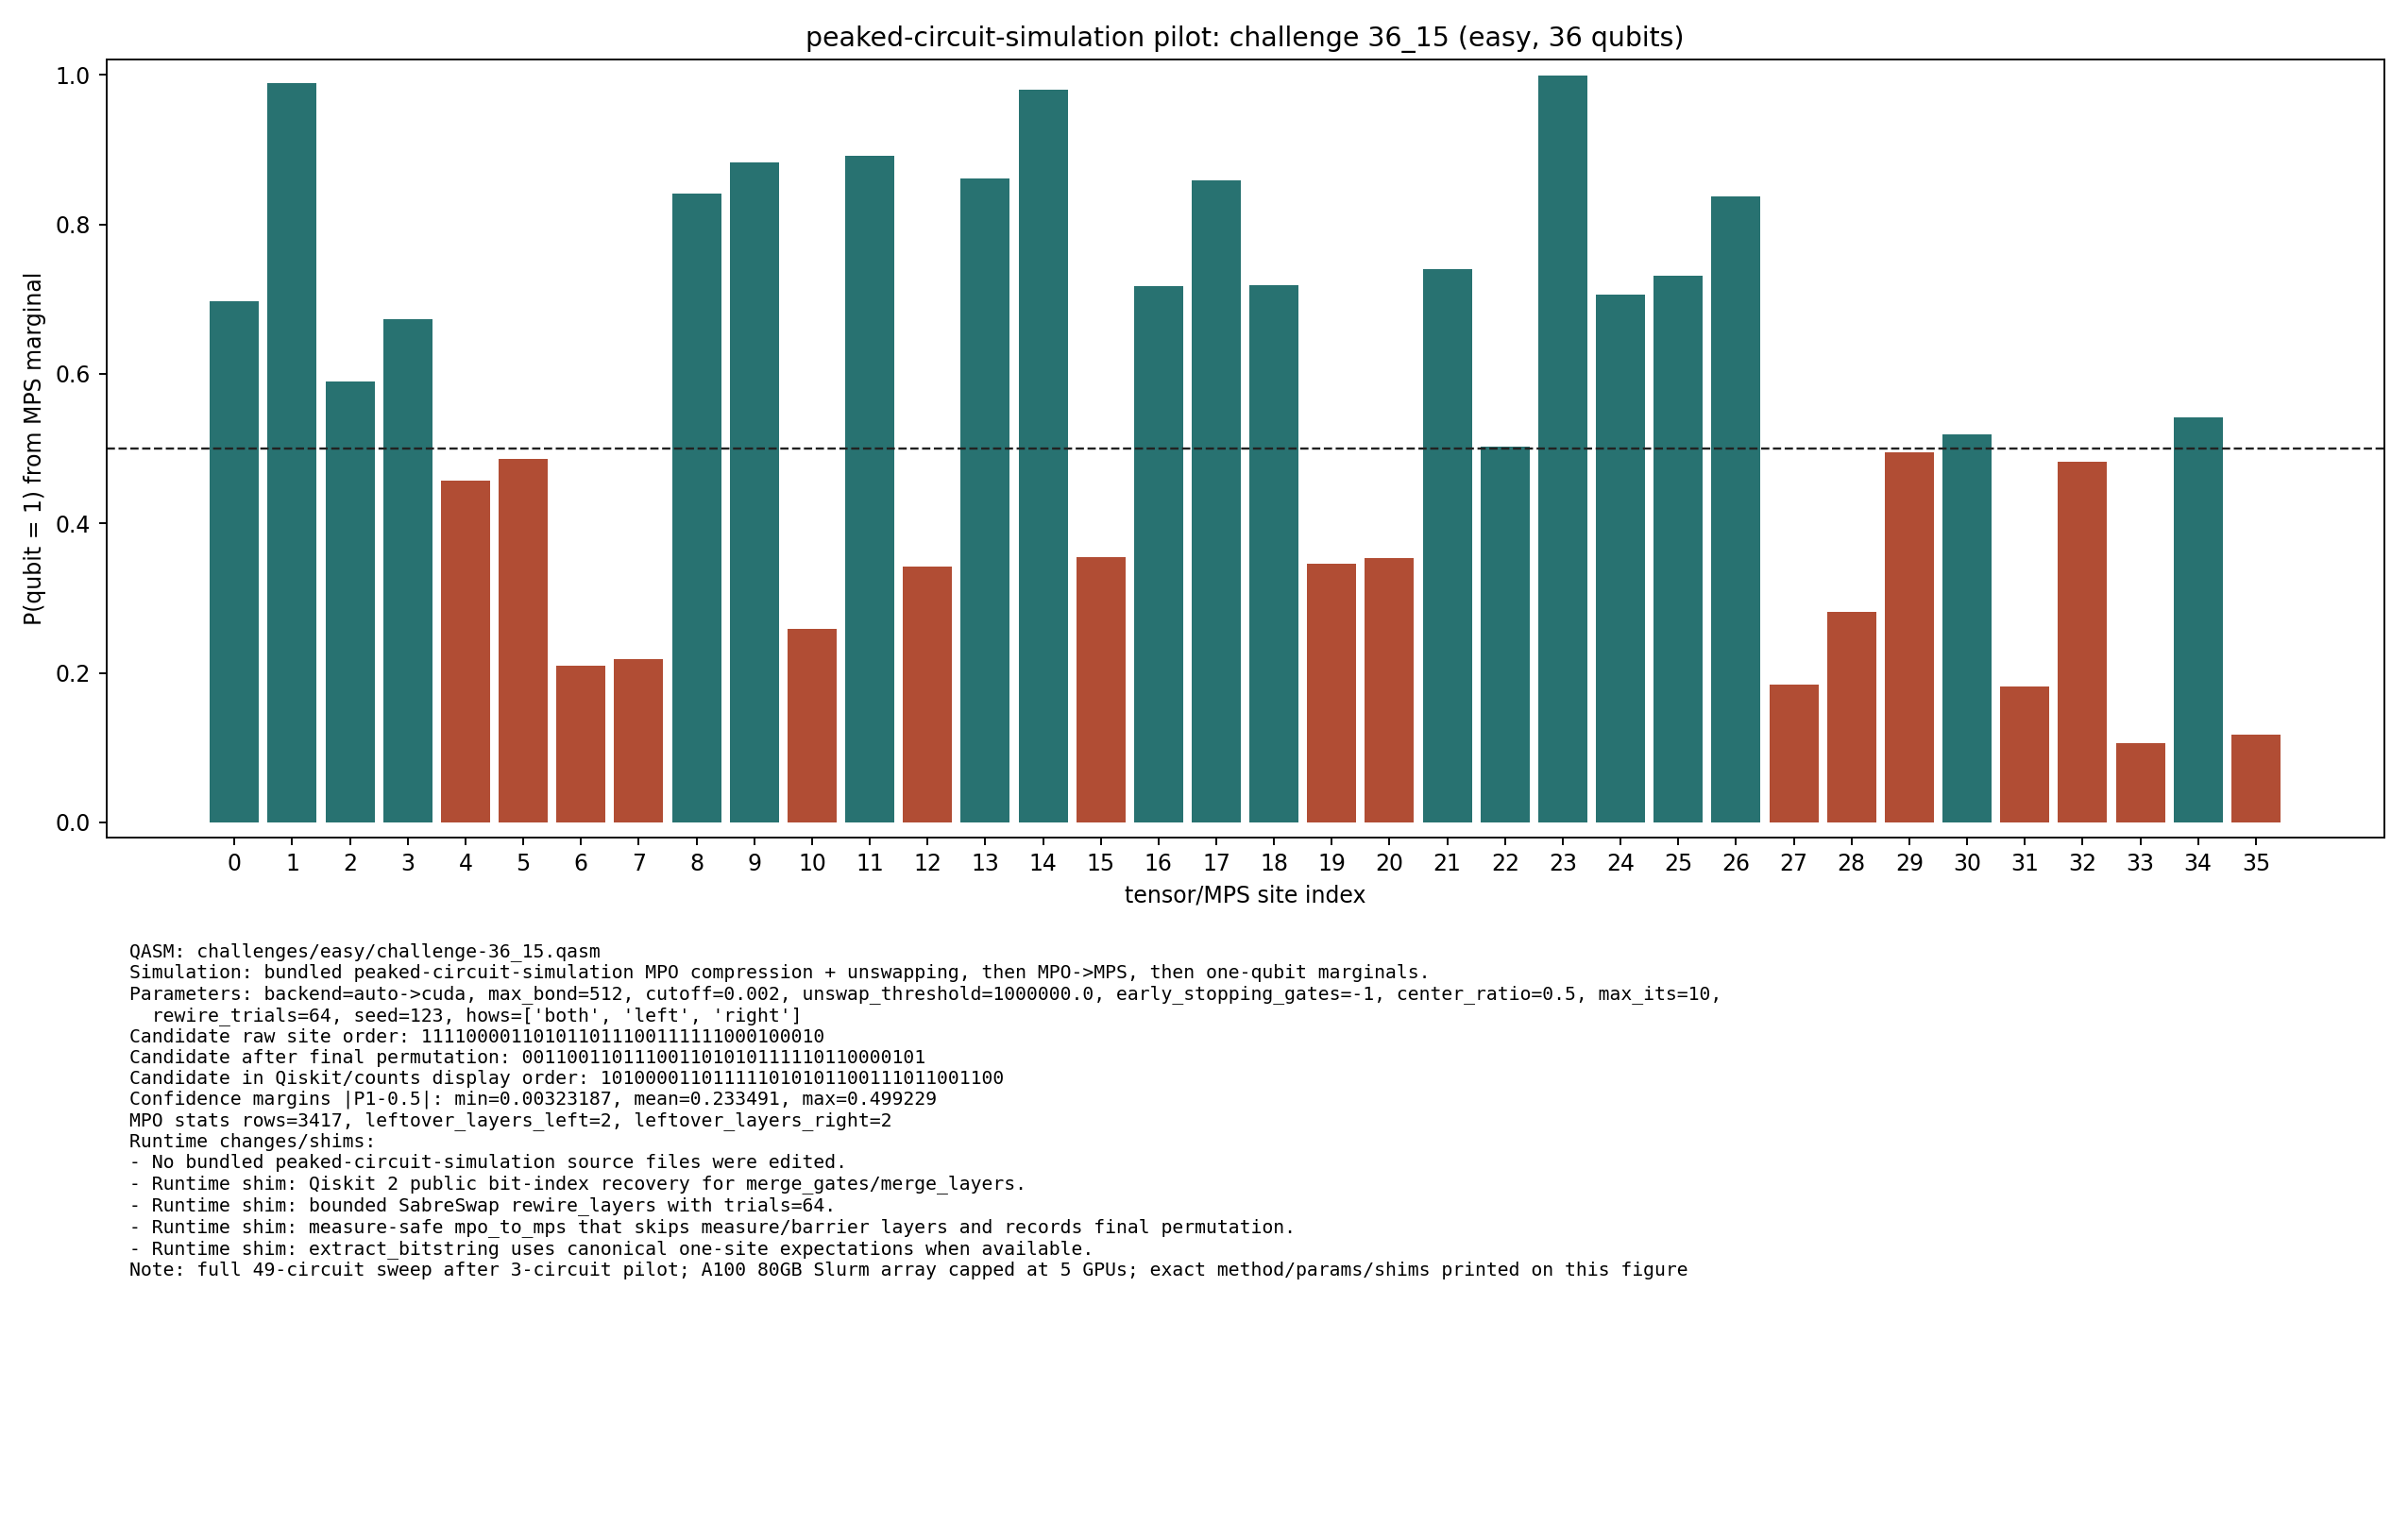
\includegraphics[width=\linewidth]{figures/appendix_peaked_36_15.png}
\caption*{\code{36\_15}: per-qubit marginal distribution.}
\end{minipage}
\caption{\code{peaked-circuit-simulation} marginal distributions.}
\end{figure}

\begin{figure}[H]
\centering
\begin{minipage}{0.48\linewidth}
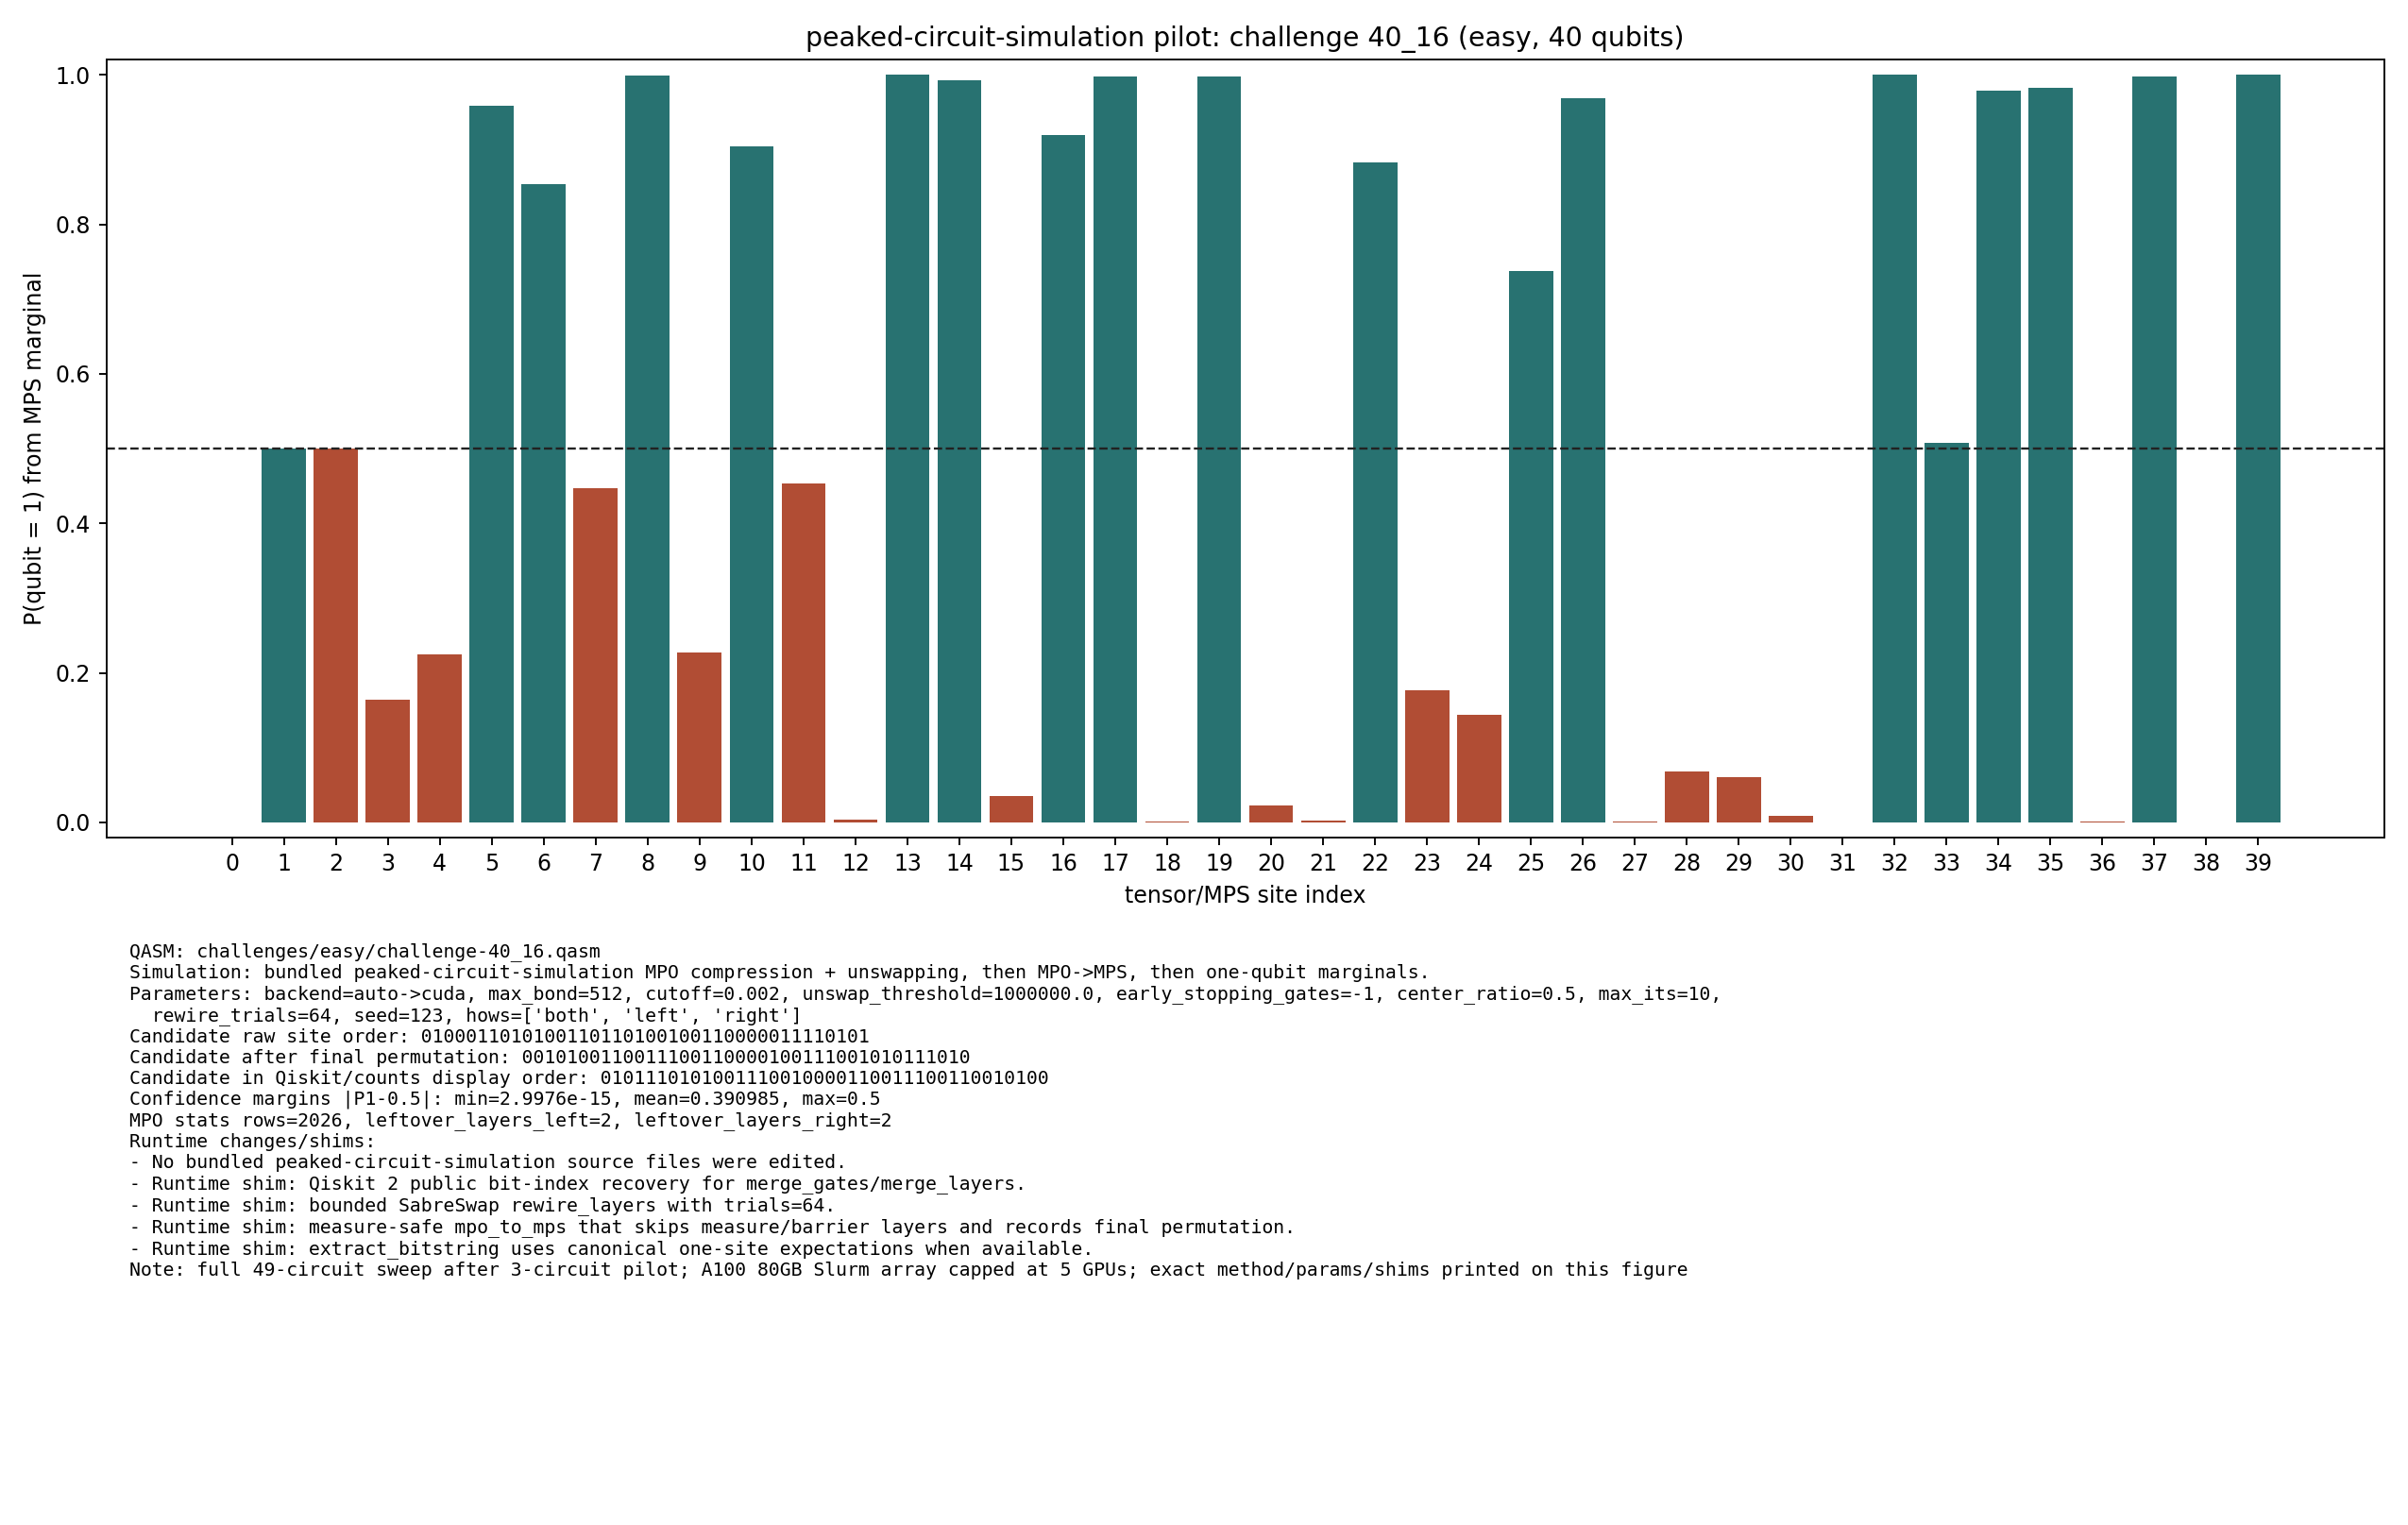
\includegraphics[width=\linewidth]{figures/appendix_peaked_40_16.png}
\caption*{\code{40\_16}: per-qubit marginal distribution.}
\end{minipage}\hfill
\begin{minipage}{0.48\linewidth}
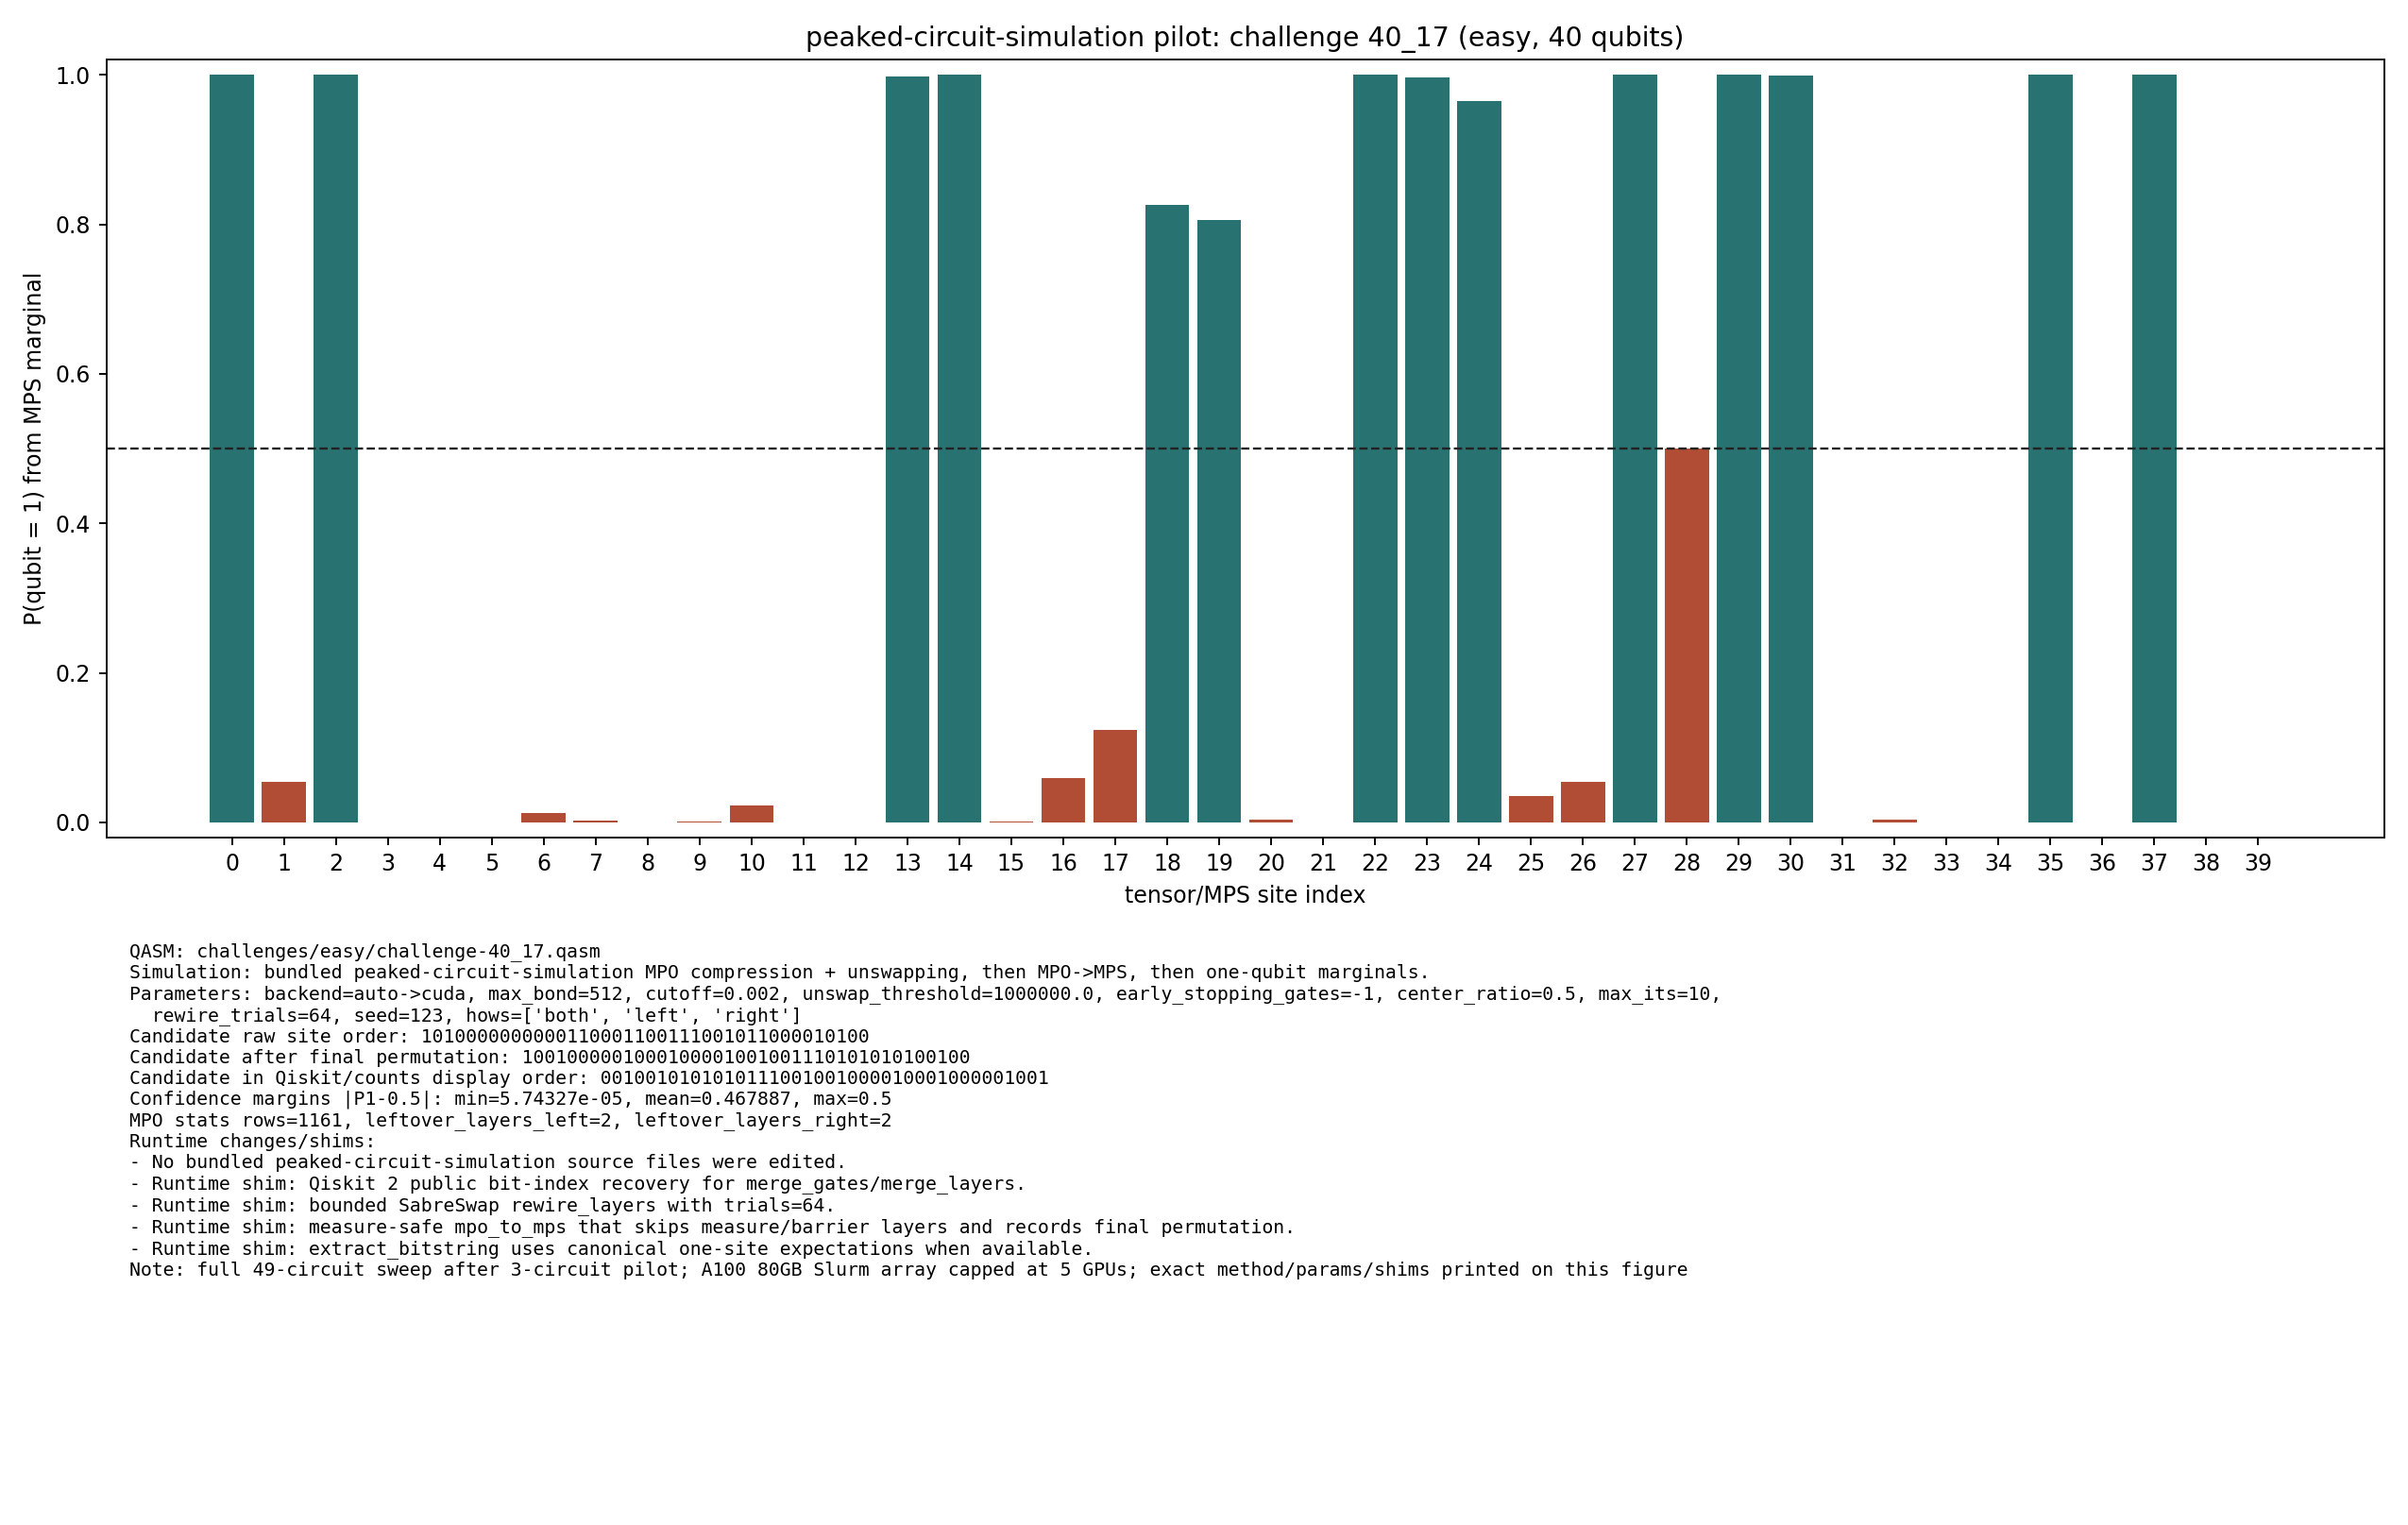
\includegraphics[width=\linewidth]{figures/appendix_peaked_40_17.png}
\caption*{\code{40\_17}: per-qubit marginal distribution.}
\end{minipage}
\caption{\code{peaked-circuit-simulation} marginal distributions.}
\end{figure}

\begin{figure}[H]
\centering
\begin{minipage}{0.48\linewidth}
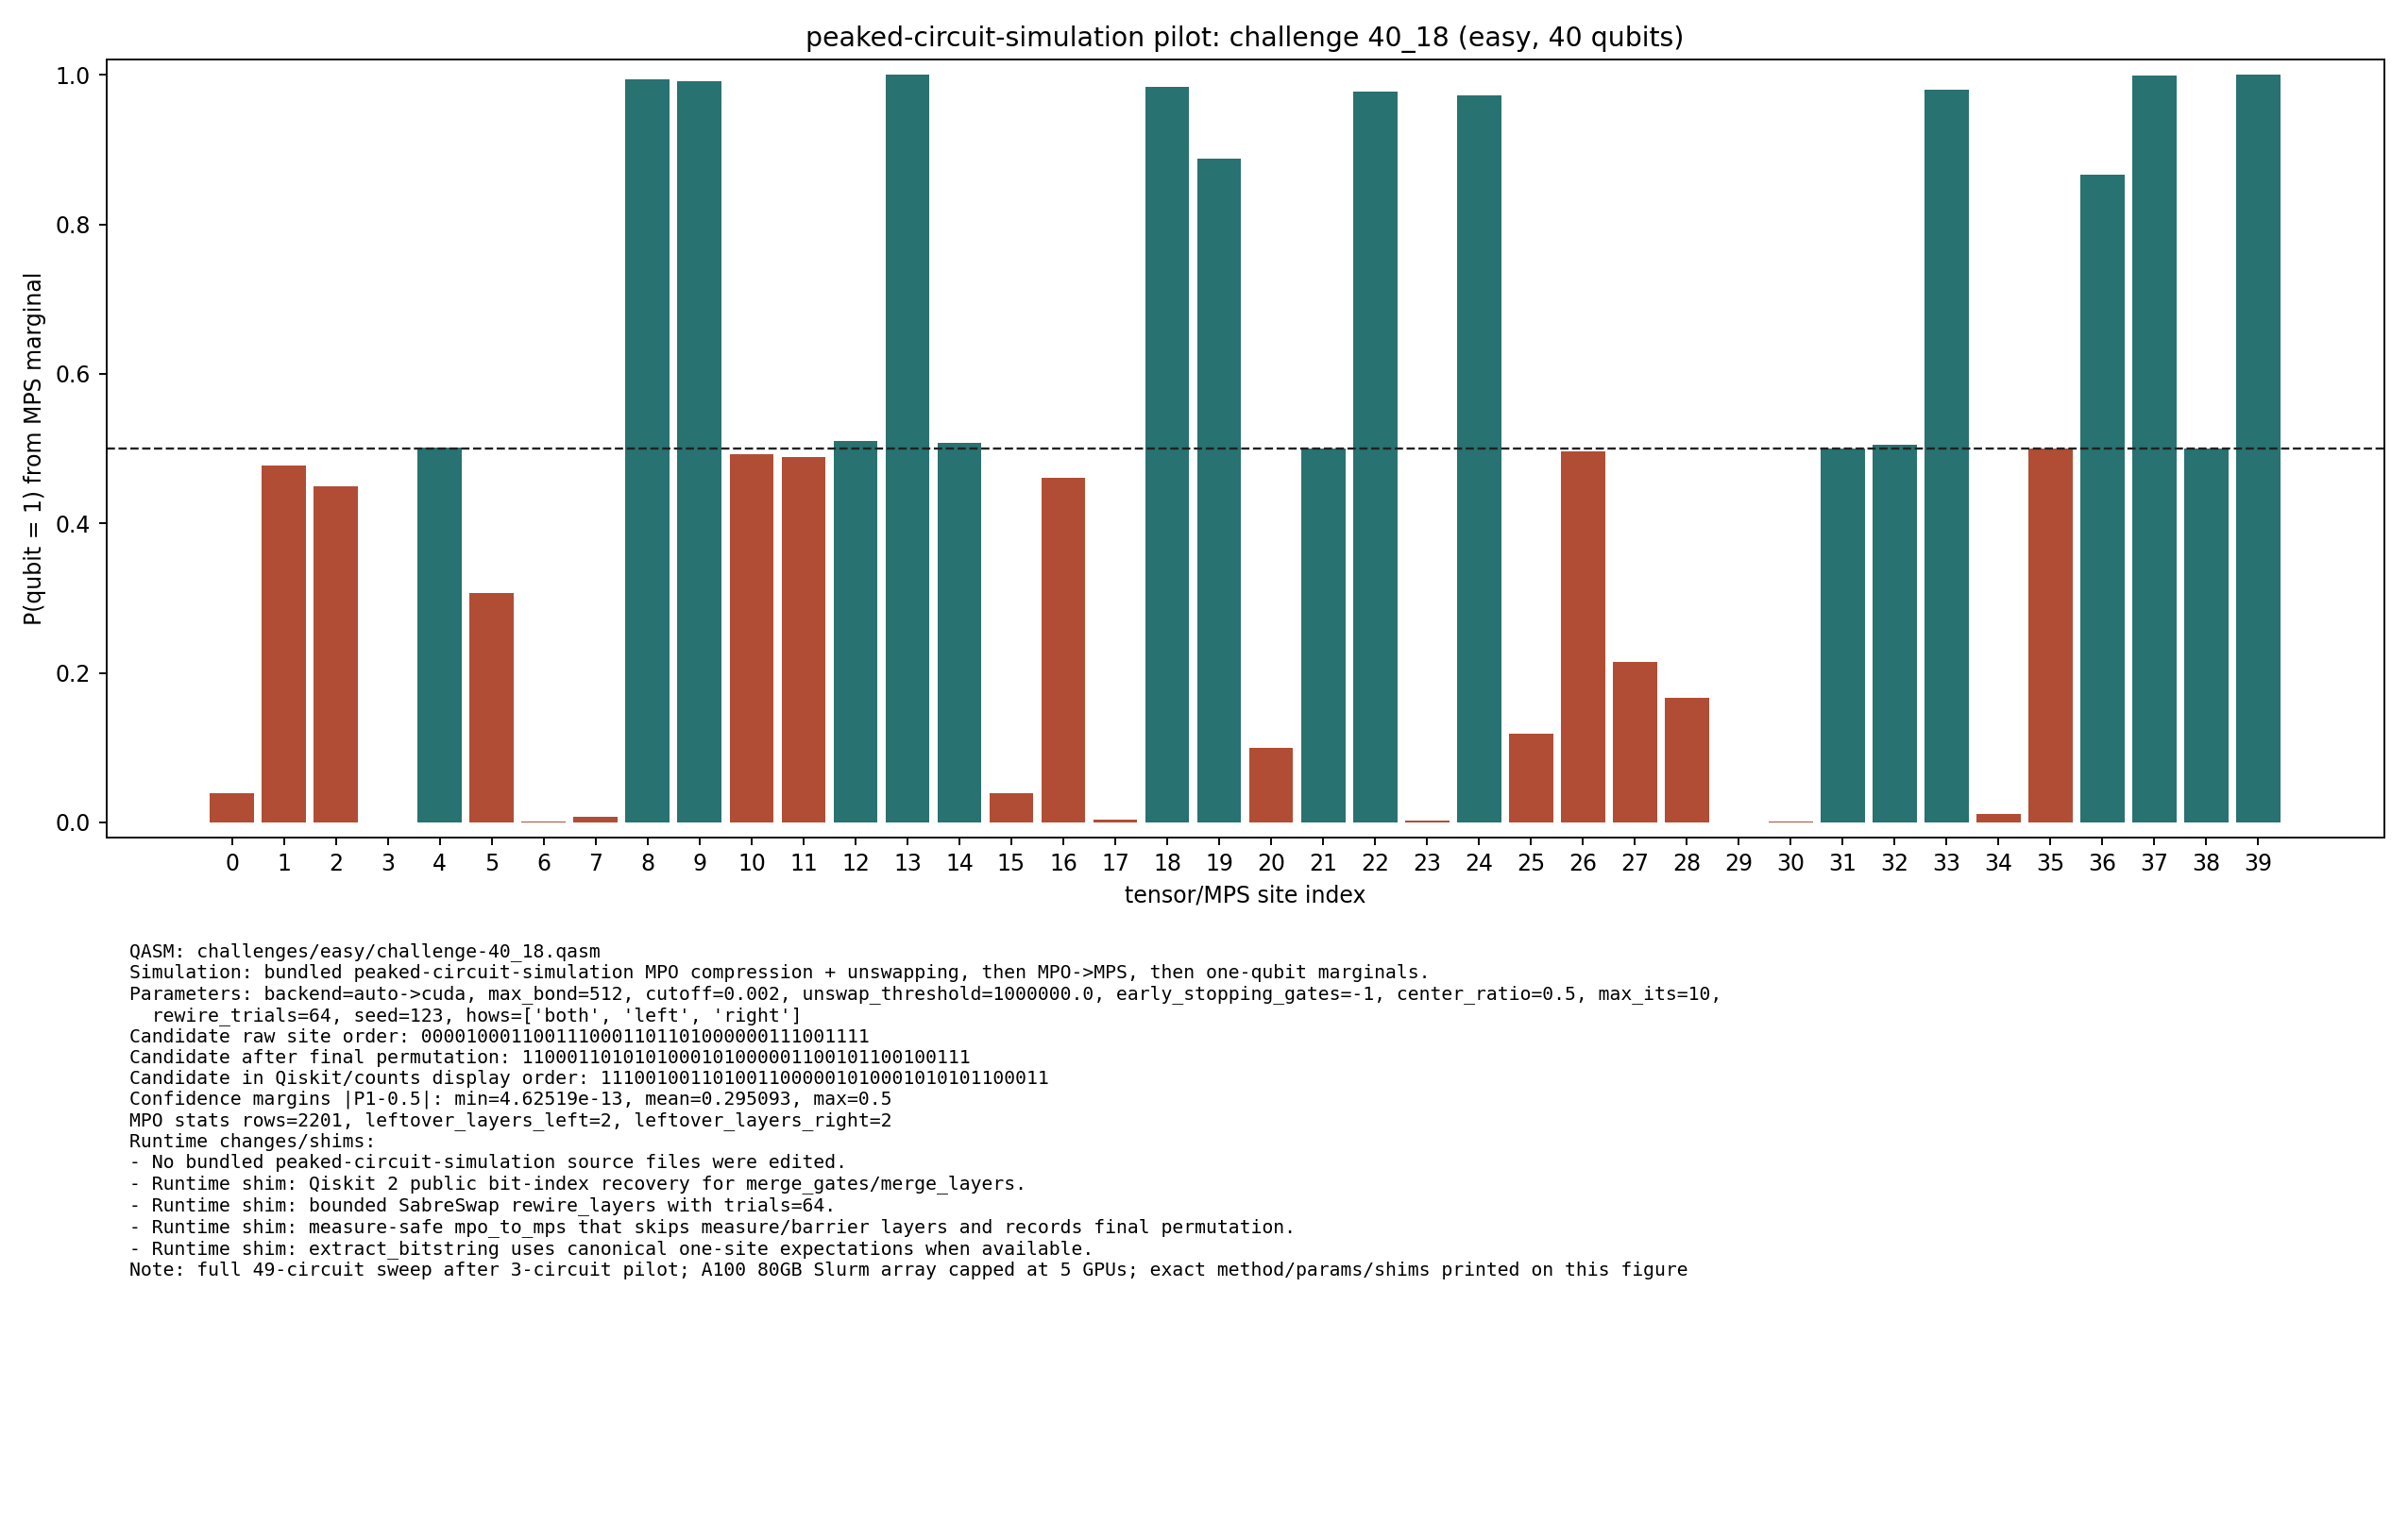
\includegraphics[width=\linewidth]{figures/appendix_peaked_40_18.png}
\caption*{\code{40\_18}: per-qubit marginal distribution.}
\end{minipage}\hfill
\begin{minipage}{0.48\linewidth}
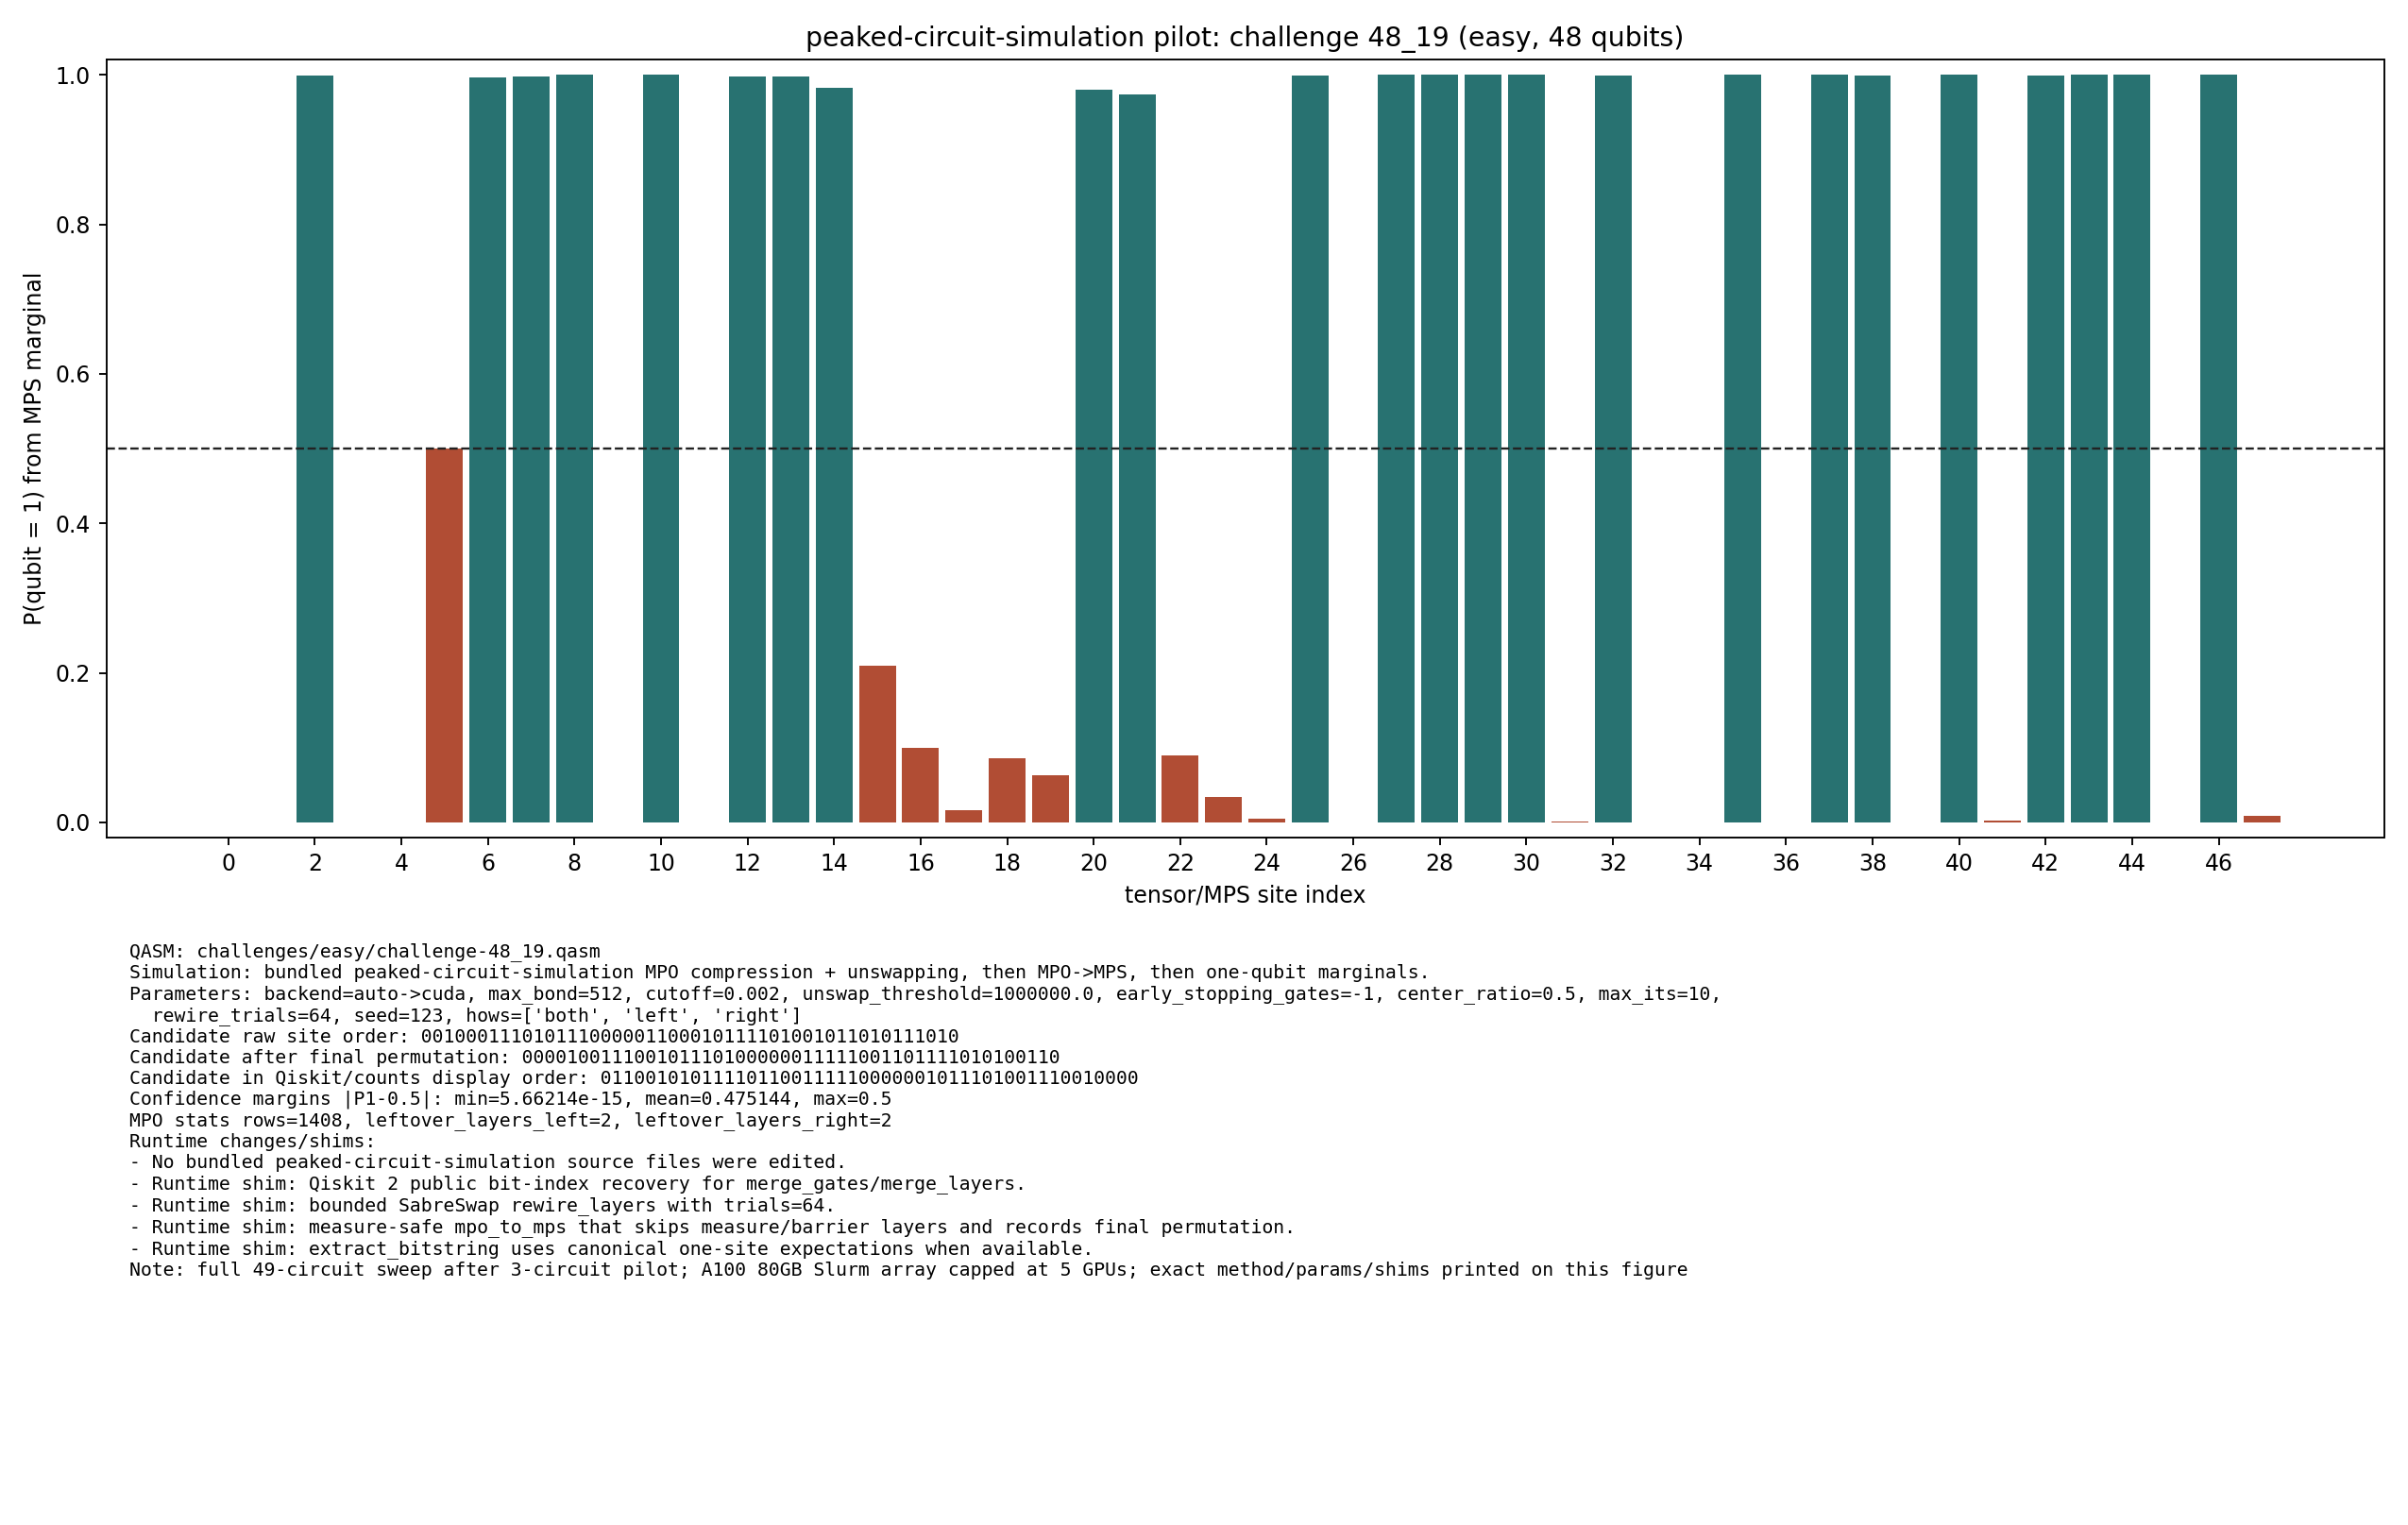
\includegraphics[width=\linewidth]{figures/appendix_peaked_48_19.png}
\caption*{\code{48\_19}: per-qubit marginal distribution.}
\end{minipage}
\caption{\code{peaked-circuit-simulation} marginal distributions.}
\end{figure}

\begin{figure}[H]
\centering
\begin{minipage}{0.48\linewidth}
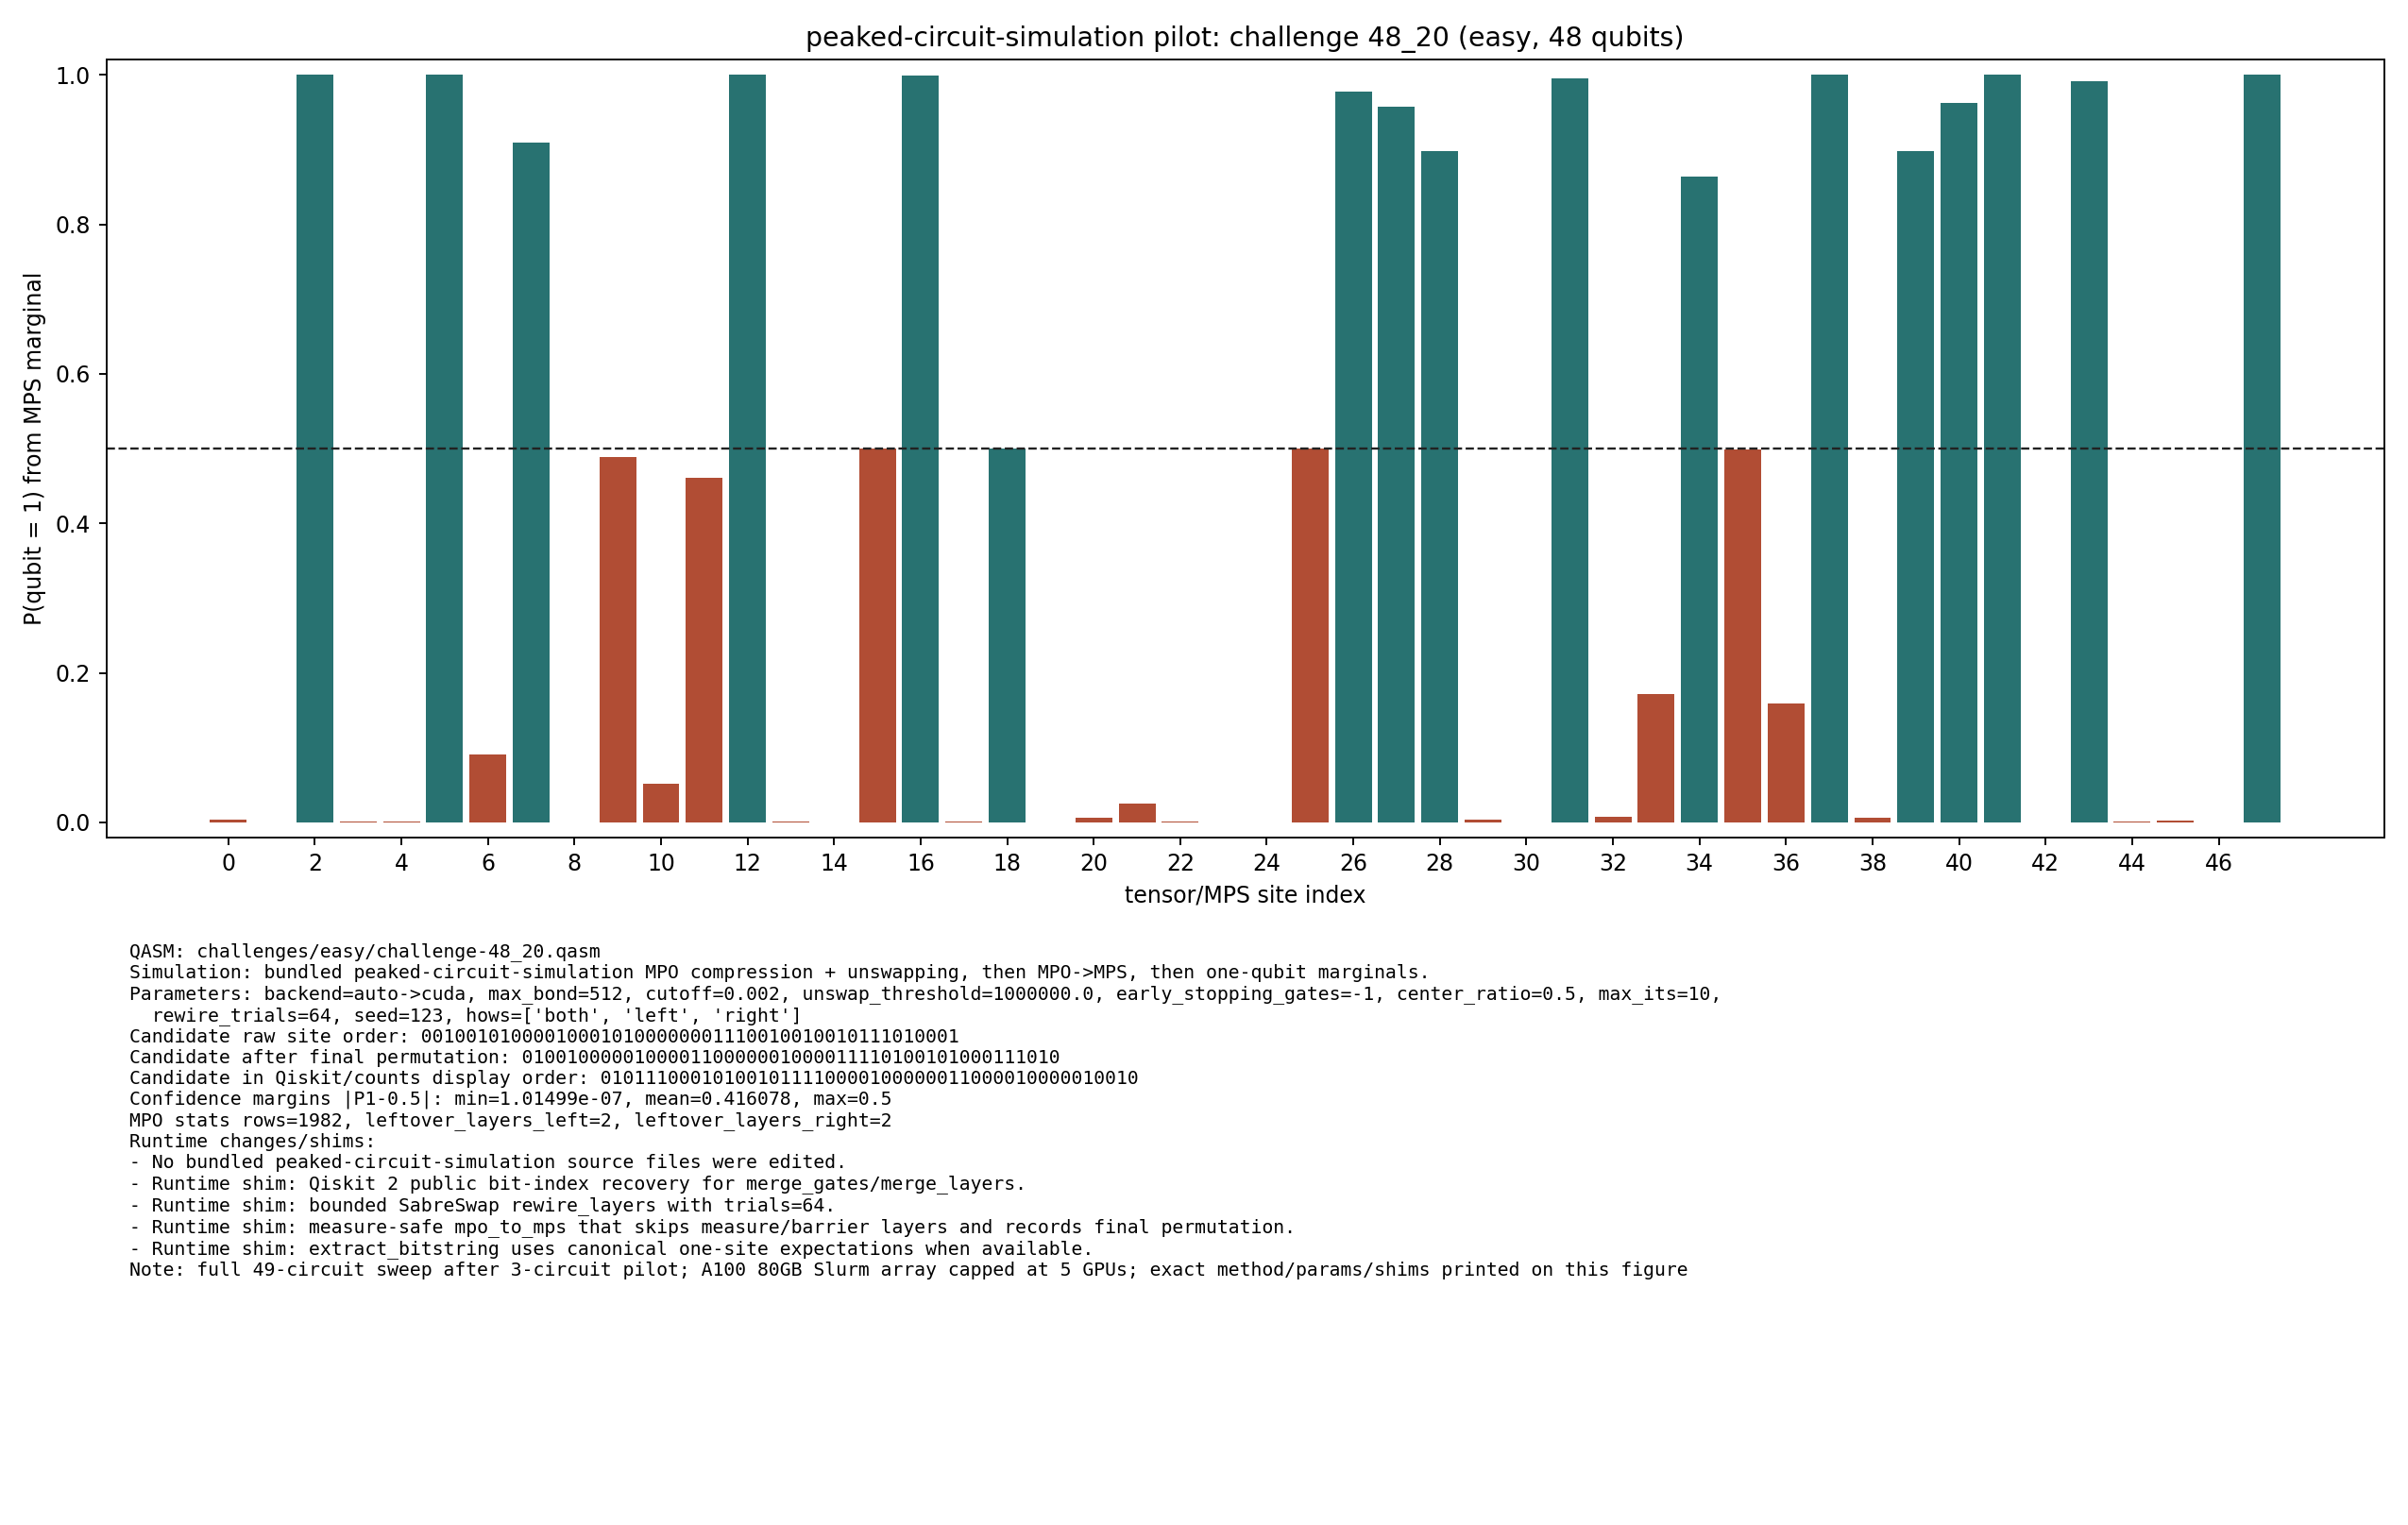
\includegraphics[width=\linewidth]{figures/appendix_peaked_48_20.png}
\caption*{\code{48\_20}: per-qubit marginal distribution.}
\end{minipage}\hfill
\begin{minipage}{0.48\linewidth}
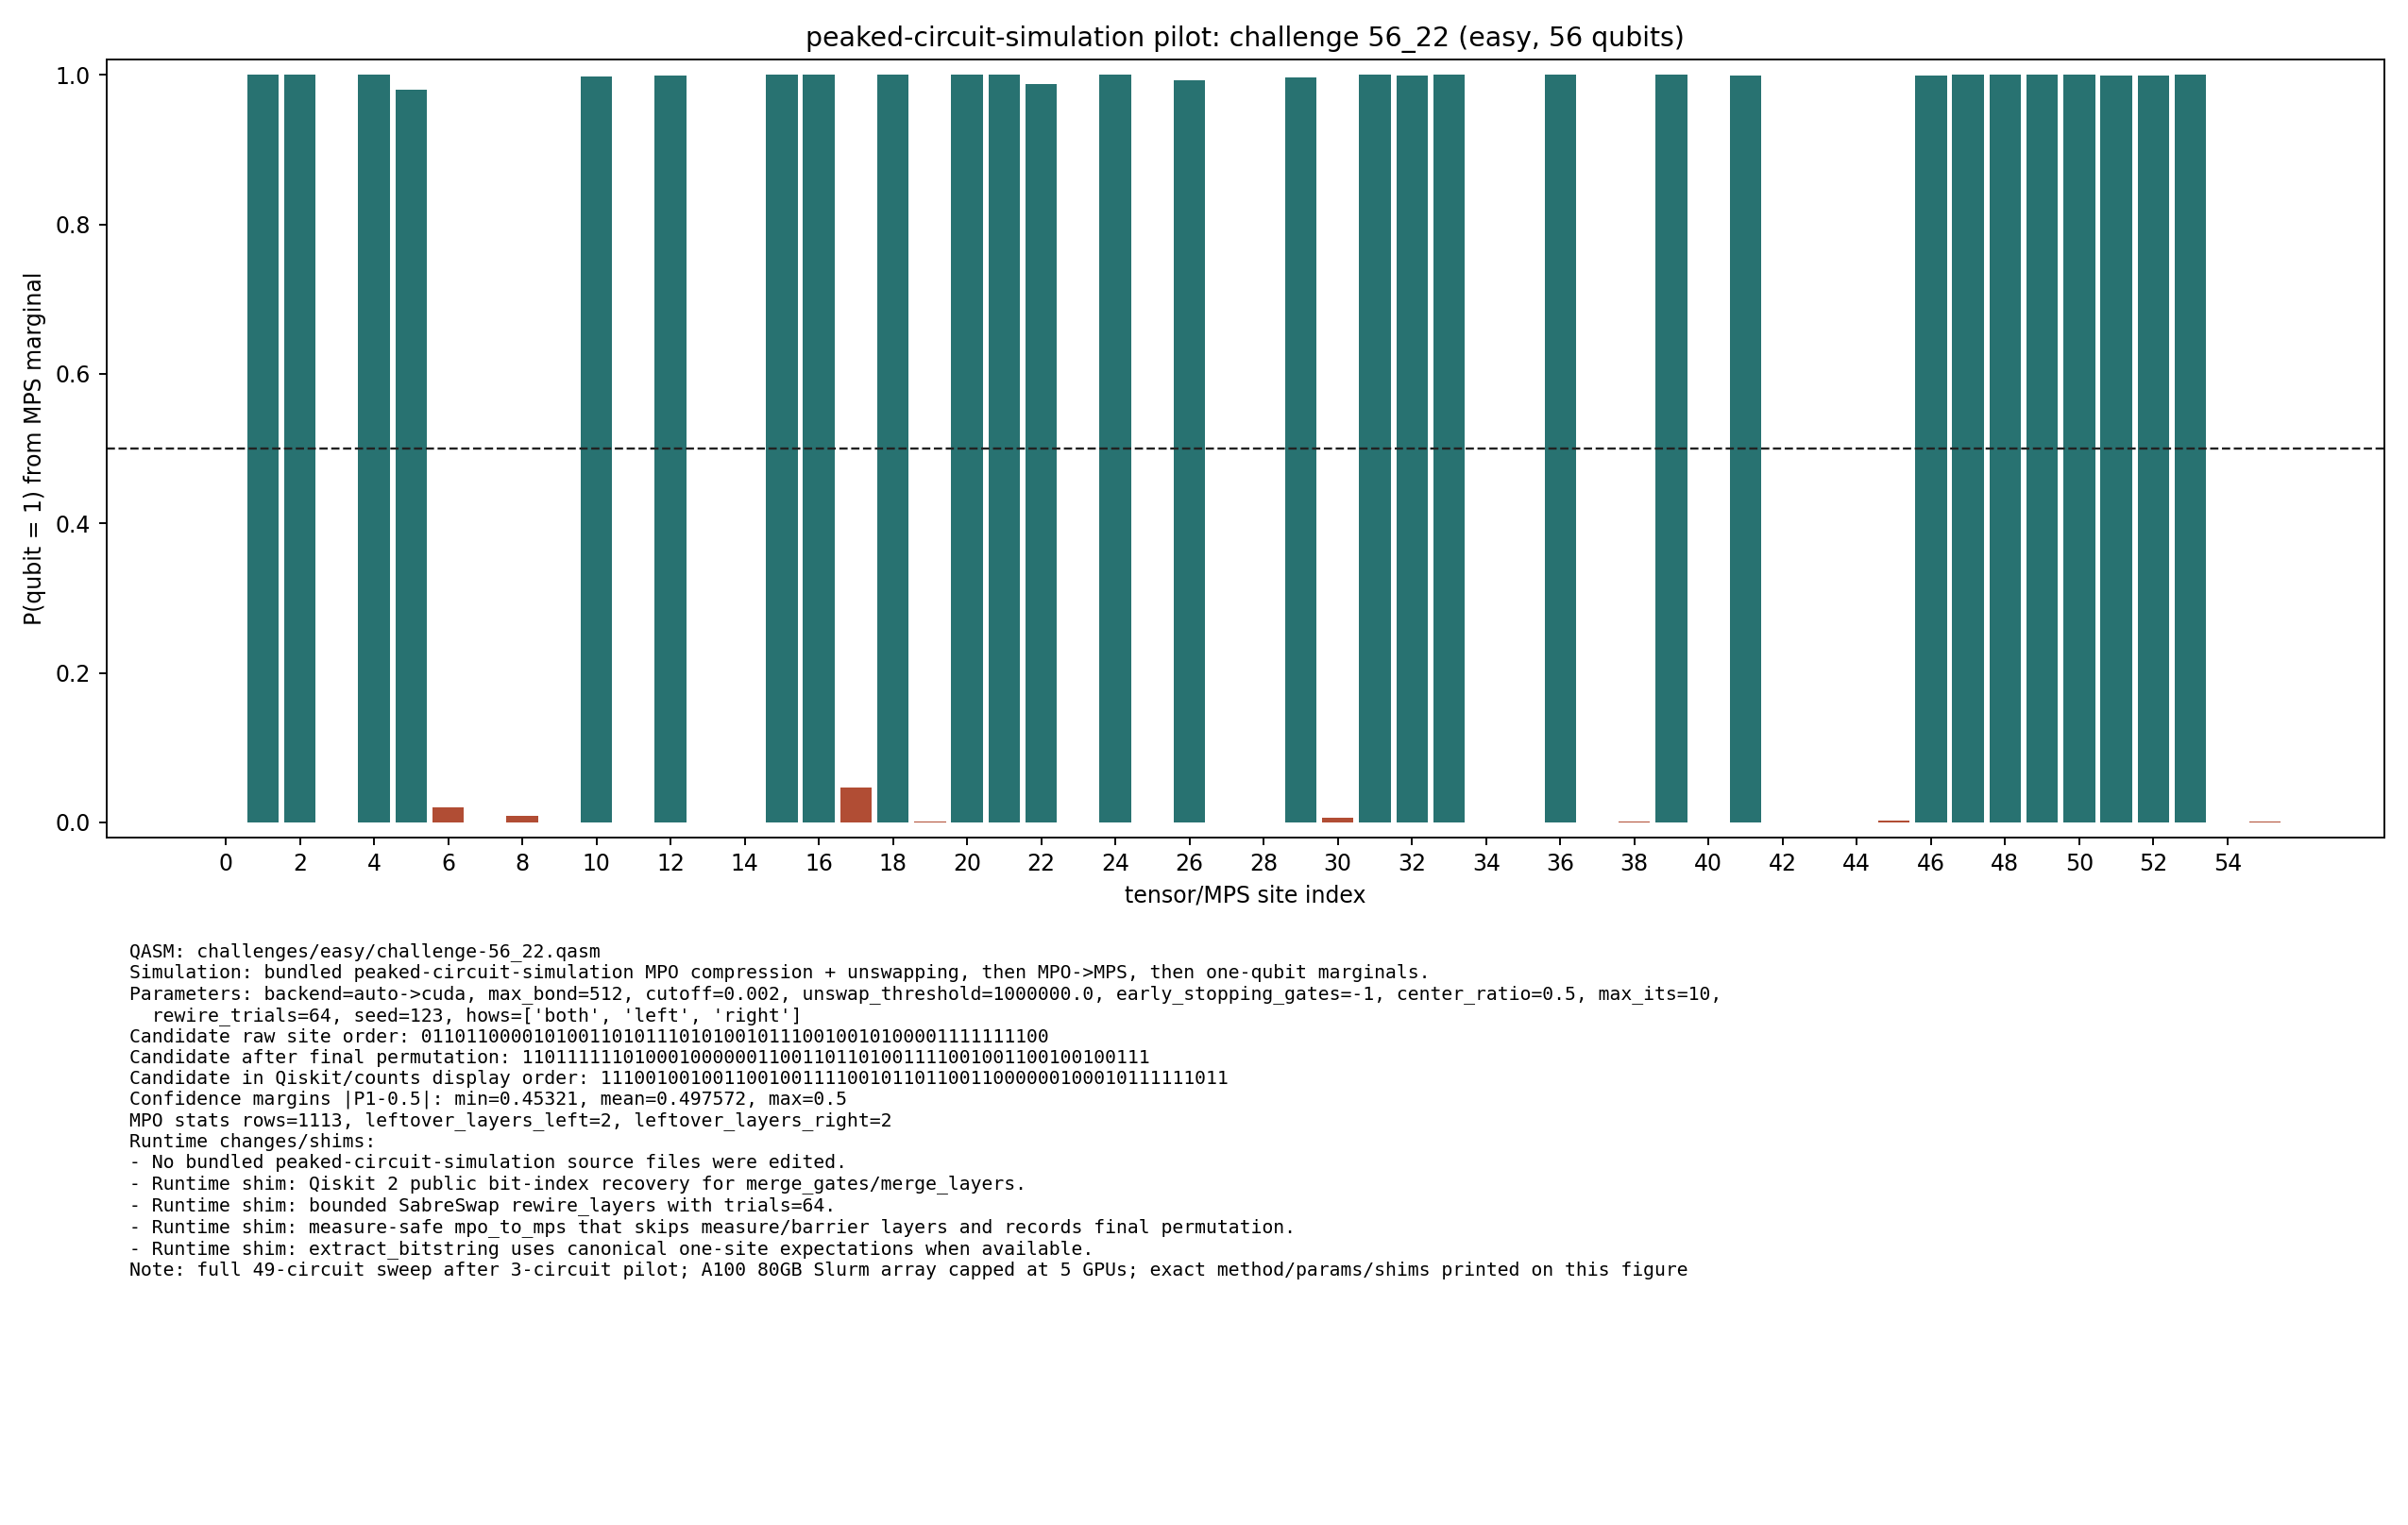
\includegraphics[width=\linewidth]{figures/appendix_peaked_56_22.png}
\caption*{\code{56\_22}: per-qubit marginal distribution.}
\end{minipage}
\caption{\code{peaked-circuit-simulation} marginal distributions.}
\end{figure}

\begin{figure}[H]
\centering
\begin{minipage}{0.48\linewidth}
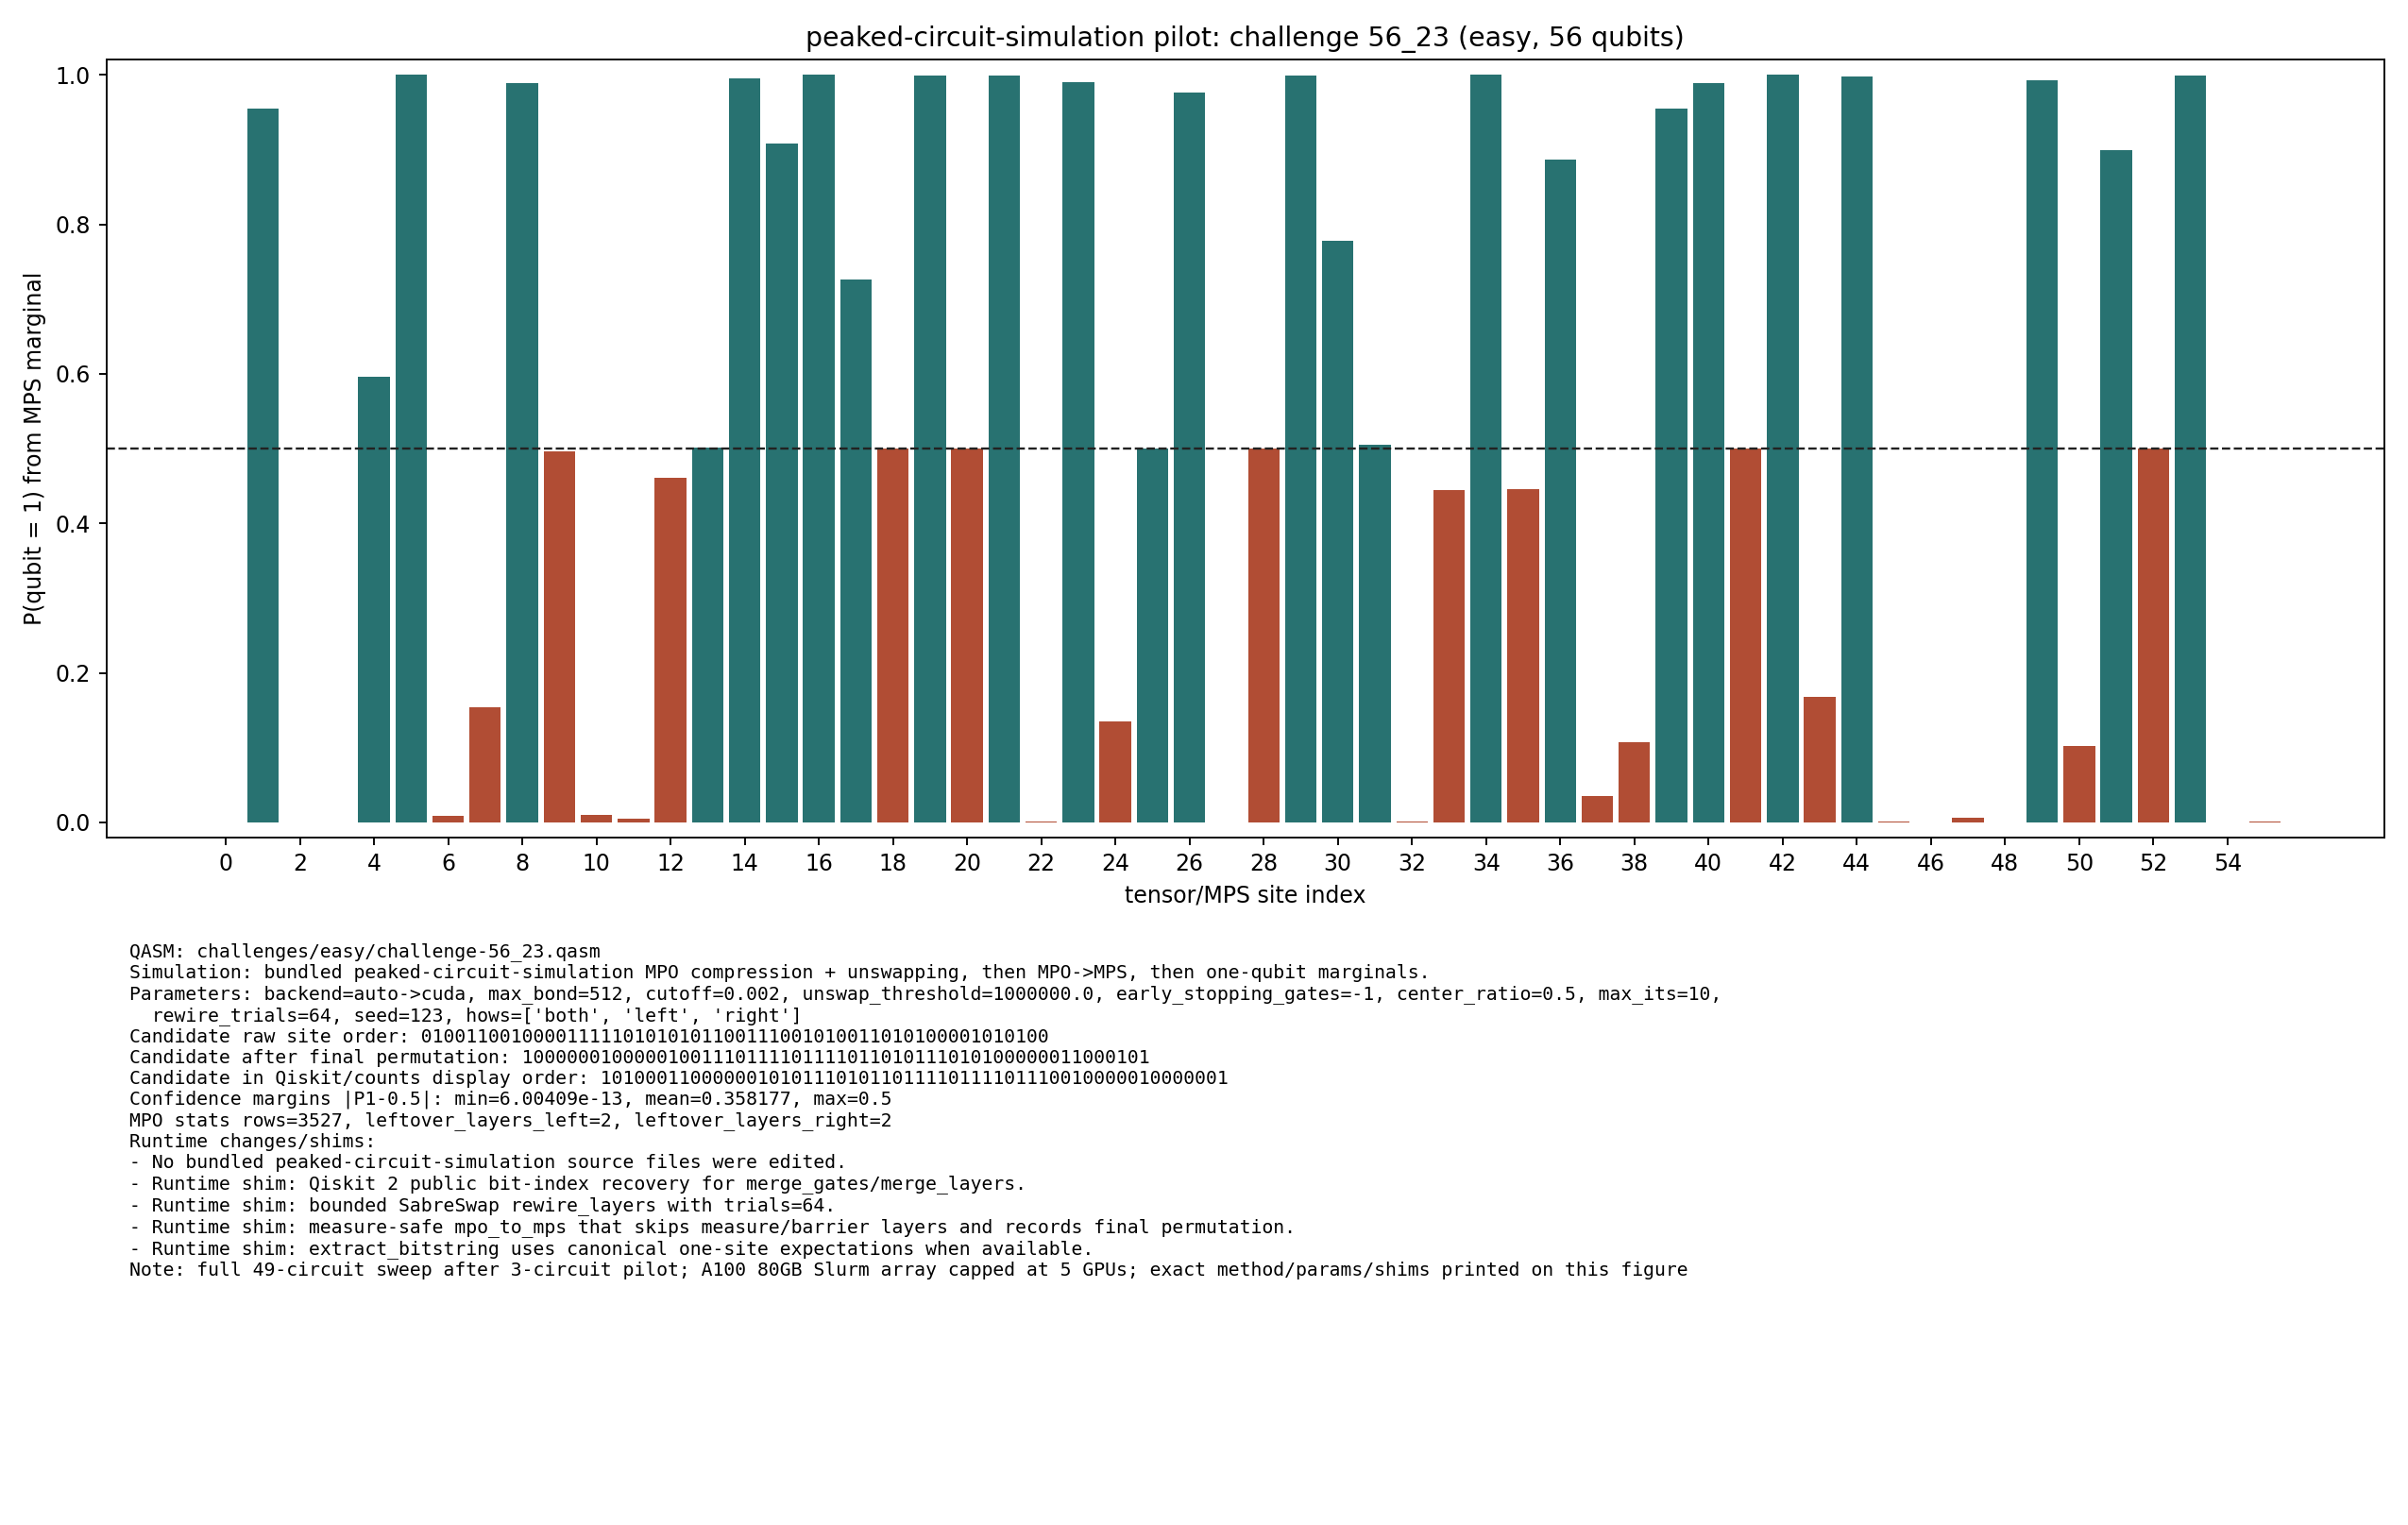
\includegraphics[width=\linewidth]{figures/appendix_peaked_56_23.png}
\caption*{\code{56\_23}: per-qubit marginal distribution.}
\end{minipage}\hfill
\begin{minipage}{0.48\linewidth}
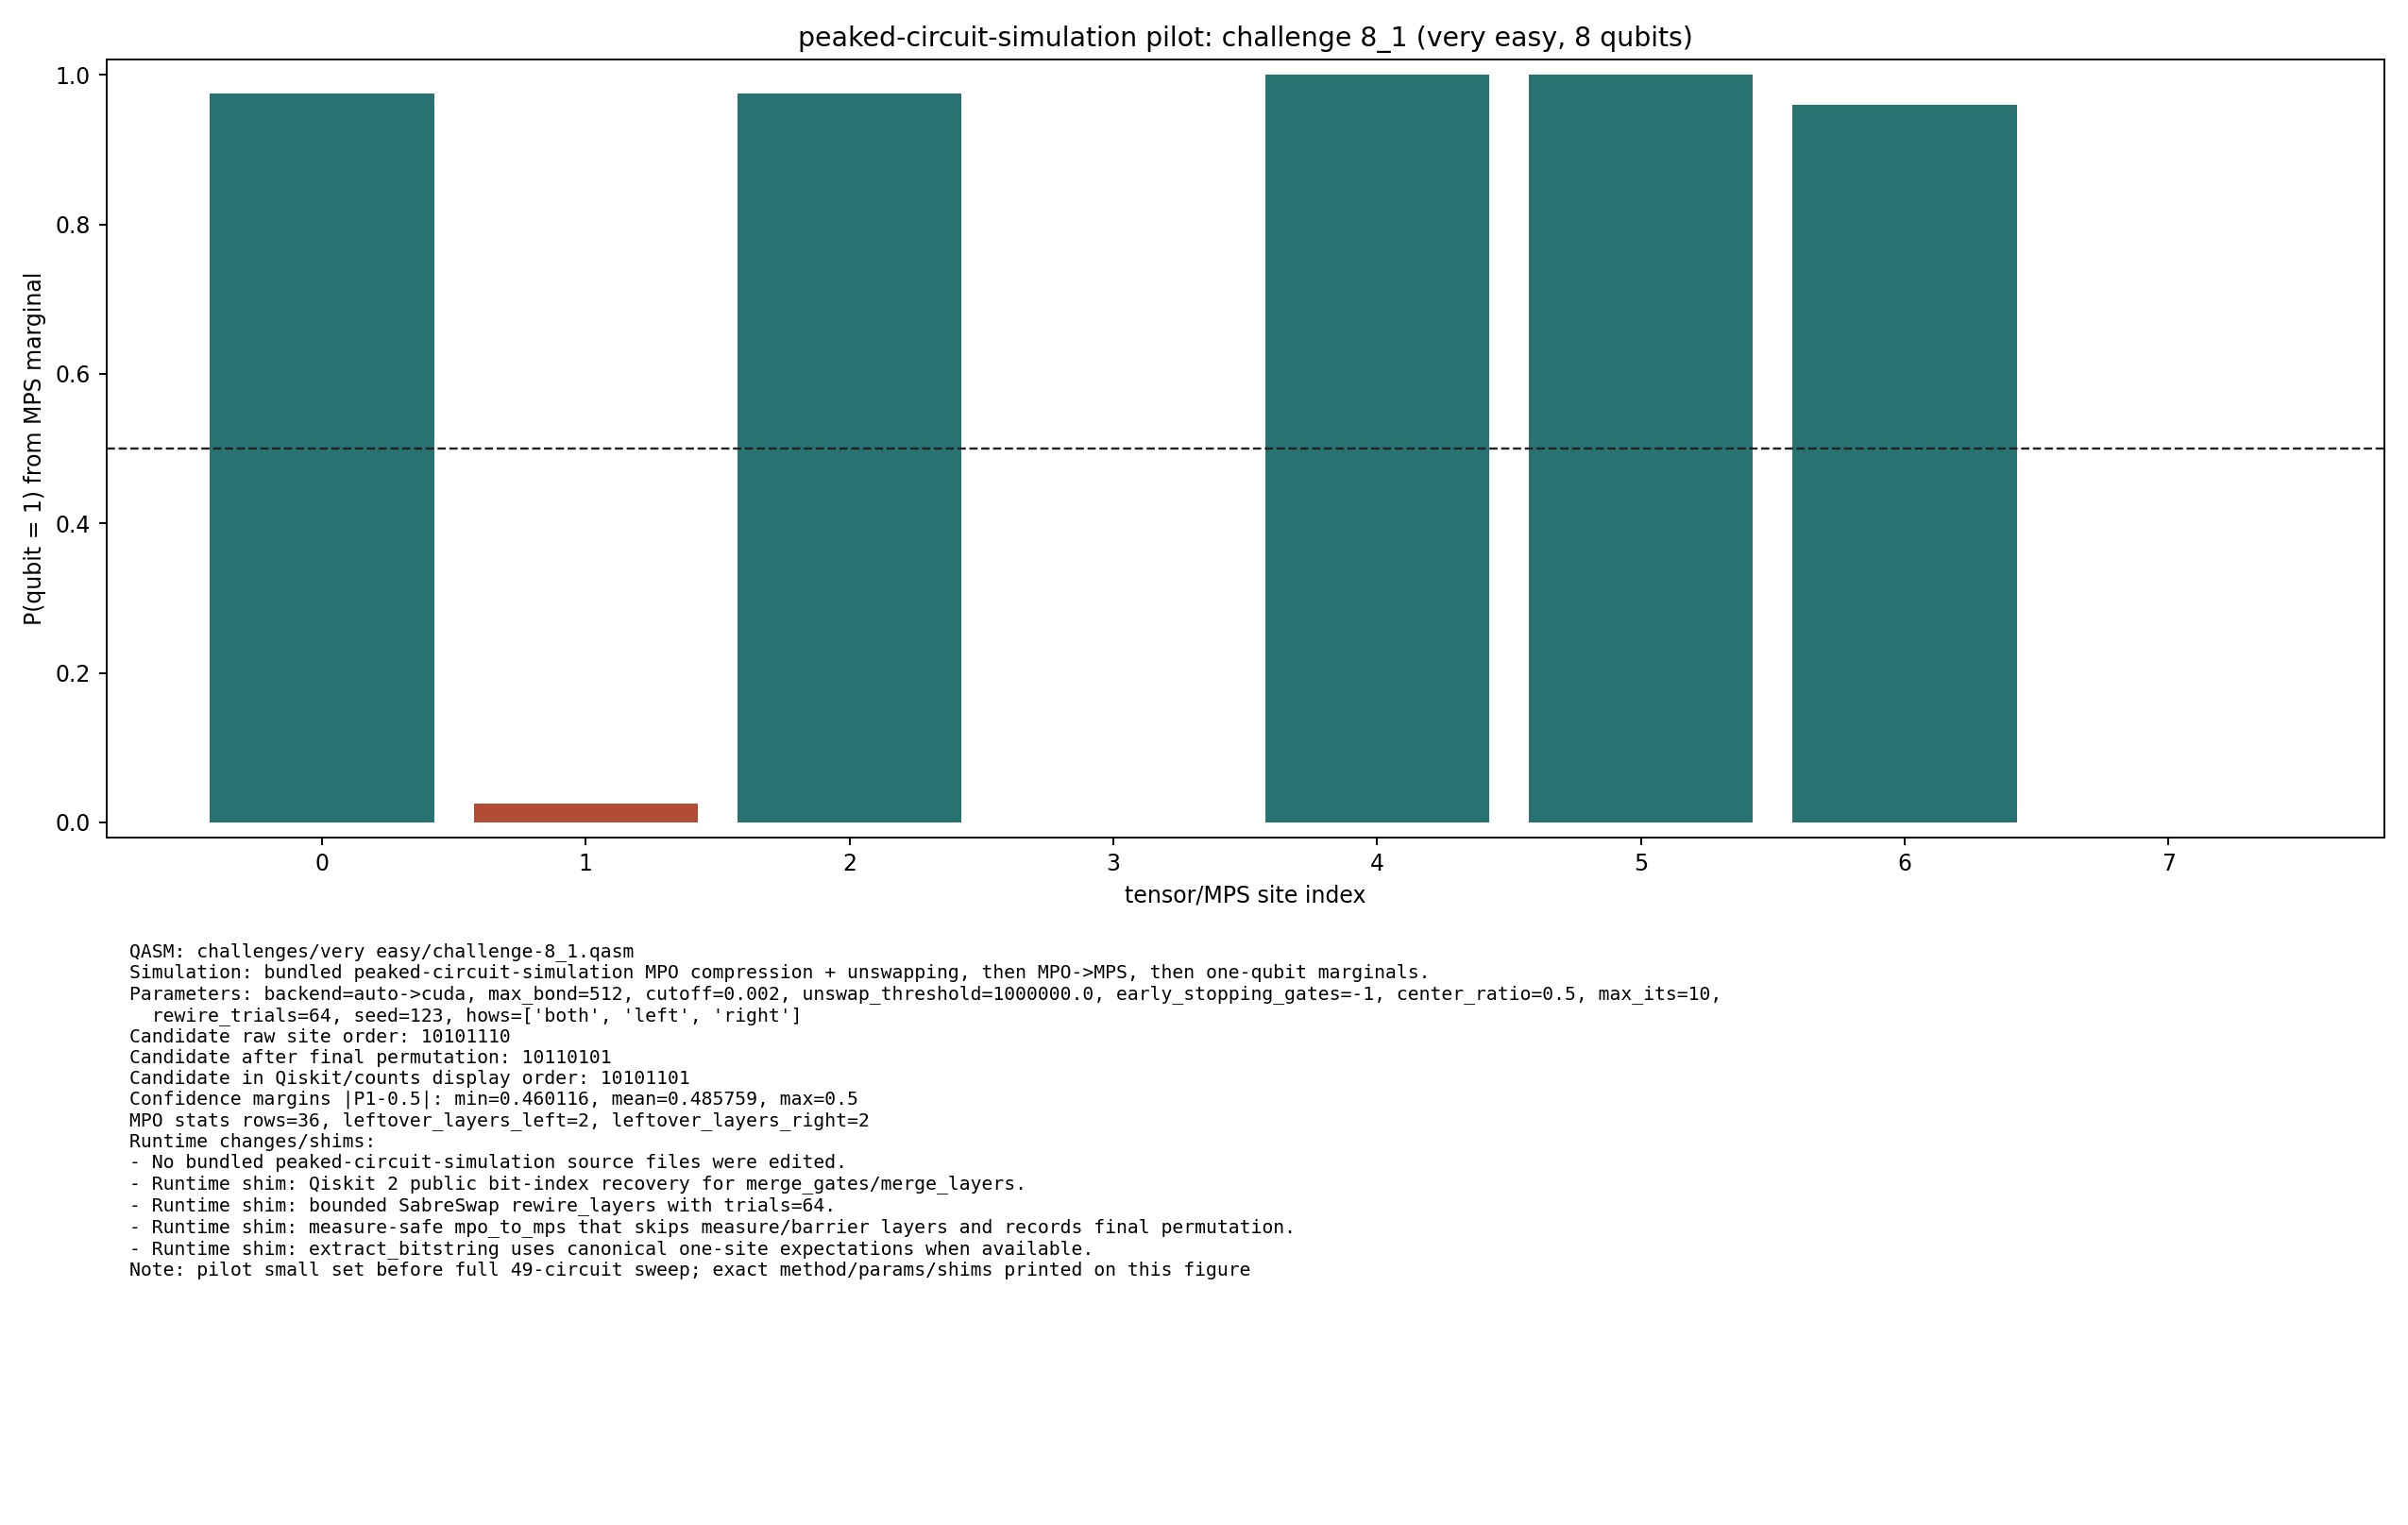
\includegraphics[width=\linewidth]{figures/appendix_peaked_8_1.png}
\caption*{\code{8\_1}: per-qubit marginal distribution.}
\end{minipage}
\caption{\code{peaked-circuit-simulation} marginal distributions.}
\end{figure}

\begin{figure}[H]
\centering
\begin{minipage}{0.48\linewidth}
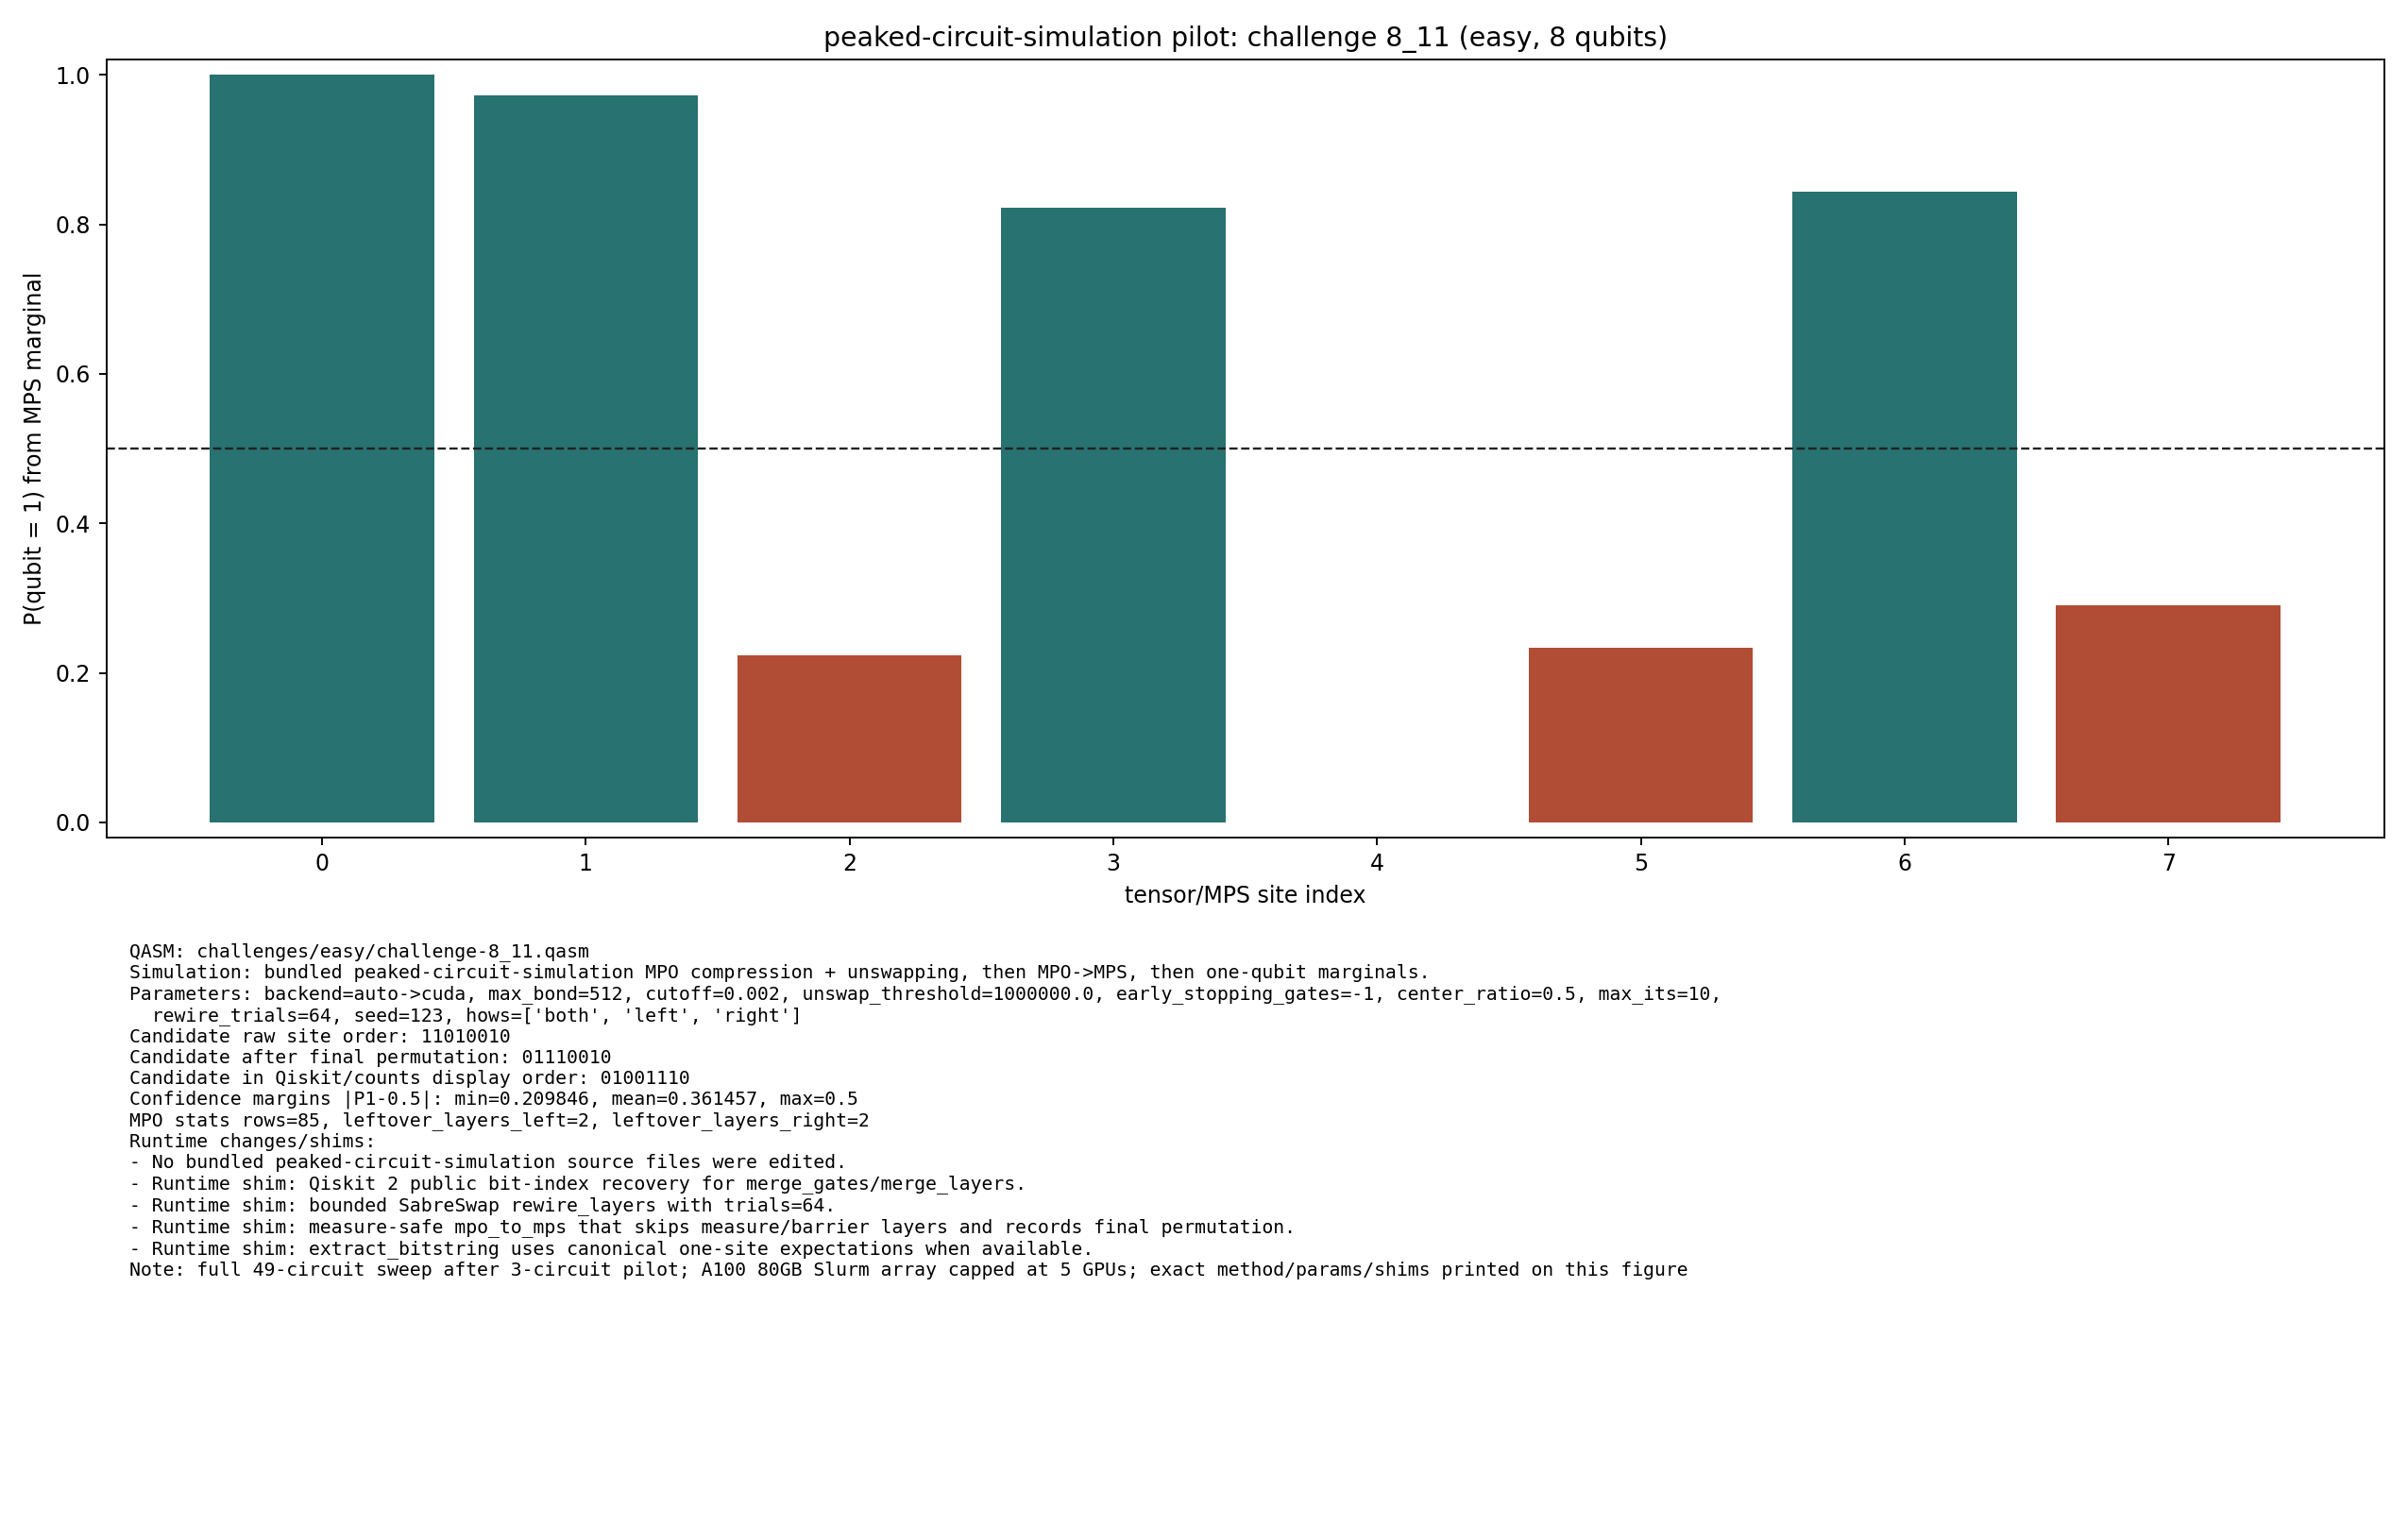
\includegraphics[width=\linewidth]{figures/appendix_peaked_8_11.png}
\caption*{\code{8\_11}: per-qubit marginal distribution.}
\end{minipage}\hfill
\begin{minipage}{0.48\linewidth}
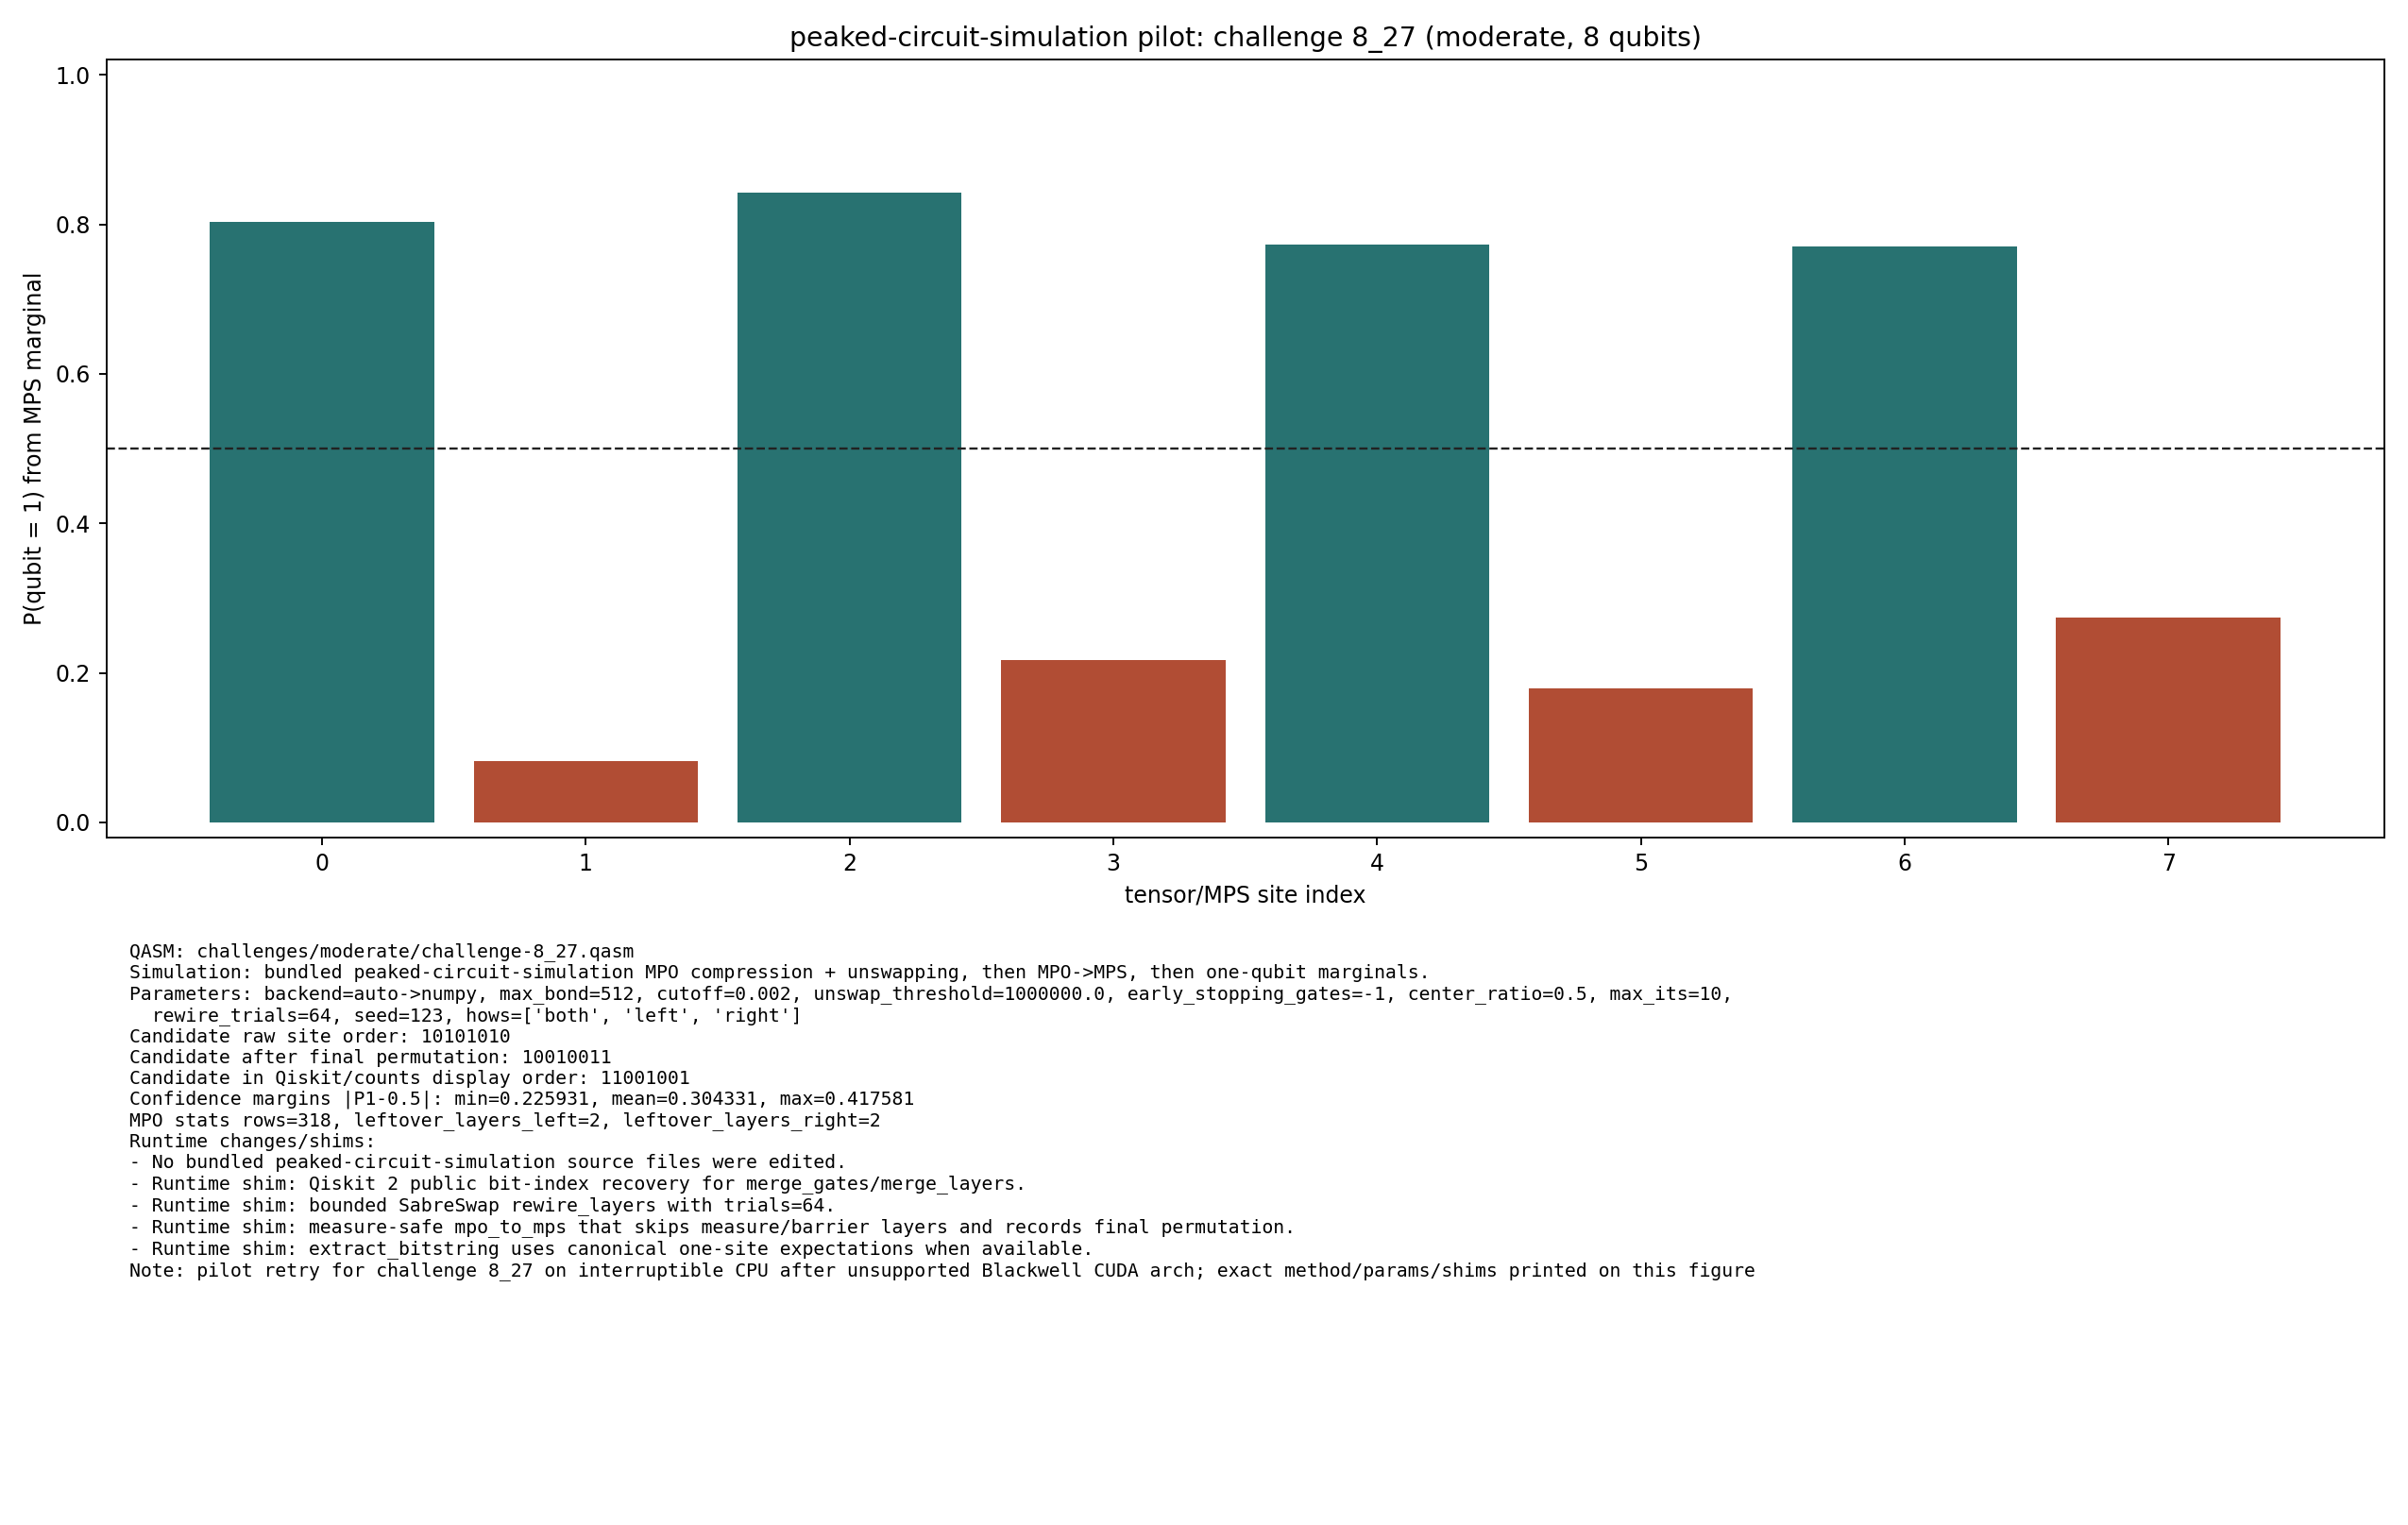
\includegraphics[width=\linewidth]{figures/appendix_peaked_8_27.png}
\caption*{\code{8\_27}: per-qubit marginal distribution.}
\end{minipage}
\caption{\code{peaked-circuit-simulation} marginal distributions.}
\end{figure}

\subsection{Partial or Missing Peaked-Circuit Results}
The full peaked sweep did not complete. It left 9 \code{started} JSON files and 28 missing outputs after Slurm cancellation. Those entries have no valid distribution plot and should not be interpreted as answers. The completed marginal plots above are the complete usable visual set from the peaked-circuit run in this session.
